%%%%%%%%%%%%%%%%%%%%%%%%%%%%%%%%%%%%%%%%%%%%%%%%%%%%%%%%%%%
% EPFL report package, main thesis file
% Goal: provide formatting for theses and project reports
% Author: Mathias Payer <mathias.payer@epfl.ch>
%
% To avoid any implication, this template is released into the
% public domain / CC0, whatever is most convenient for the author
% using this template.
%
%%%%%%%%%%%%%%%%%%%%%%%%%%%%%%%%%%%%%%%%%%%%%%%%%%%%%%%%%%%
\documentclass[a4paper,11pt,oneside]{report}
% Options: MScThesis, BScThesis, MScProject, BScProject
\usepackage[MScThesis,lablogo]{EPFLreport}
\usepackage{xspace}
\usepackage{amsmath}
\usepackage{subcaption}
\usepackage[T1]{fontenc}

\title{Self-supervised learning\\for calcium segmentation on coronary OCT images}
\author{Naravich Chutisilp}
\supervisor{Karim Kadry, Ph.D. candidate}
\adviser{Professor Elazer R. Edelman, M.D., Ph.D.}
\coadviser{Professor Maria Brbi\'c, Ph.D.}
\expert{Farhad Rikhtegar Nezami, Ph.D.}

% \newcommand{\sysname}{FooSystem\xspace}

\dedication{
    \begin{raggedleft}
        It’s no use going back to yesterday, because I was a different person then.\\
        --- Lewis Carroll, Alice’s Adventures in Wonderland\\
    \end{raggedleft}
    \vspace{4cm}
    \begin{center}
        Dedicated to my lovely family, my dear friends, and kind people who have given opportunity and support to this lucky life I have.
    \end{center}
}
\acknowledgments{
% This is where you thank those who supported you on this journey. Good examples
% are your significant other, family, advisers, and other parties that inspired
% you during this project. Generally, this section is about 1/2 page to a page.

% Consider acknowledging the use and location of this thesis package.

% Define your acknowledgments in \texttt{\textbackslash{}acknowledgments\{...\}}
% and show them with \texttt{\textbackslash{}makeacks}.

    I would like to show my deep gratitude to my mom and dad for their unwavering support and firm trust in letting me choose my path. I would love to thank my two lovely sisters, Namking and Namkow, for their continuous love and understanding. 

    I am also grateful to all the friends I have made during my time at EPFL, Set, James, Kwang, Ice, Sundae, Nai, Cindy, Jenestin, Thomas, Paulina, Fah, Ting-Wei, Pin-Yen, Yi-Kai, Hong-Bin, Leo, Edvin, Anthon, Aamir, Jirka, and many more people I have not mentioned, who have made my life abroad memorable and amicable. Going to EPFL is my first time living abroad for more than a month and I could not have asked for a better experience than what I have had. Simple dinners in the evening every day after school, meaningful conversations about everything, and trips to alpine mountains and European cities have made this little boy feel accompanied in the middle of the unknown future.

    Furthermore, I could not forget the friends I have made during my time at MIT, Mee, Pooh, Cue, and Champ who have made my final Master's semester fun and unforgettable. Coming to MIT is a dream come true, yet it was not easy to leave my friends in Switzerland and start anew in the US. Unexpectedly, since the first day I arrived, I was welcomed with open arms and was shown to many places in Boston. Worries and fears were replaced with excitement and joy. Hiking in the White Mountains, visiting California and Silicon Valley, walking along the Freedom Trail, enjoying delicacies of Lobster rolls and clam chowder, and board game night every Friday are just a few of the many memories I have made in the US that I will never forget.

    Additionally, it would not be possible if I did not have support from my friends in Thailand, Meak, Korn, Marie, Jump, Copter, Nat, Bank, Pinn, V, Poom, Pewt, Choomp, Krist, Minnie, May, Kuan and uncountable more that I could not fit into this section. Calls and messages from these lovely lives have always been a source of strength and comfort. Through tough times and good times, they have always been there for me. Even though we are 9,188 km apart, or even 13,707 km apart, it feels like they are always by my side. It is a blessing to have friends like them and I have always been grateful for that.

    I would like to thank Prof. Elazer Edelman and Karim Kadry for giving me this unparalleled opportunity to join the IMES lab at MIT and for letting me complete my Master's thesis here, as well as for providing me with advice and support on my research. 
}


\begin{document}
\maketitle
\makededication
\makeacks

\begin{abstract}
% The system tool enables the lateral decomposition of a multi-dimensional
% flux compensator along the timing and space axes.

% The abstract serves as an executive summary of your project.
% Your abstract should cover at least the following topics, 1-2 sentences for
% each: what area you are in, the problem you focus on, why existing work is
% insufficient, what the high-level intuition of your work is, maybe a neat
% design or implementation decision, and key results of your evaluation.

We studied self-supervised learning methods to improve calcium segmentation, which is crucial for treating coronary artery disease. 
This study proposes comprehensive results and comparisons of self-supervised learning and other common methods used in 3D segmentation, bridging the gap between natural and medical image self-supervised learning. We demonstrated that a convolutional neural network (CNN) is more suitable than transformers since calcium is localized and the amount of training data is small. Additionally, masked patch prediction, which is prominent in recent visual self-supervised learning, needs further refinement to be useful for medical images. We also showed that restorative task and CLIP pre-training on multi-modal co-registered images are as effective as supervised pre-training while being inexpensive. We proposed a modification to CLIP pre-training to work with multi-modal OCT images. Finally, we analyzed each pre-training approach to its determine suitability.
\end{abstract}

\maketoc

%%%%%%%%%%%%%%%%%%%%%%
\chapter{Introduction}
%%%%%%%%%%%%%%%%%%%%%%

% The introduction is a longer writeup that gently eases the reader into your
% % thesis~\cite{dinesh20oakland}. Use the first paragraph to discuss the setting.
% In the second paragraph, you can introduce the main challenge that you see.
% The third paragraph lists why related work is insufficient.
% The fourth and fifth paragraphs discuss your approach and why it is needed.
% The sixth paragraph will introduce your thesis statement. Think about how you can
% distill the essence of your thesis into a single sentence.
% The seventh paragraph will highlight some of your results
% The eighth paragraph discusses your core contribution.

% This section is usually 3-5 pages.

Numerous self-supervised learning research studies on images stem from the success of their counterparts in natural language processing (NLP). Large language models in NLP are groundbreaking inventions that allow researchers to utilize unannotated data, which is omnipresent thanks to the advent of the internet. Researchers have realized that by masking segments of text and letting the machine guess them based on the surrounding text, the machine can be used for downstream natural language tasks adeptly thereafter. Masking the text and predicting it based on its contexts is a pre-text task, a task done before the main task that does not require any human annotation. Along with text on the internet come images. However, it is unclear what pre-text tasks could be as effective as masked language modeling (MLM) in NLP. 

Visual self-supervised learning has evolved from denoising, colorizing, and solving jigsaw puzzles to aligning different views of the same image, restoring highly distorted parts of an image, and predicting the masked segments of an image by their contexts. Later, visual self-supervised learning was extended to videos, as they have more contexts to learn from than static images. Additionally, videos and 3D images share similar characteristics, with videos incorporating a temporal dimension and 3D images adding spatial depth.

Coronary artery disease (CAD) is a primary cause of heart disease caused by plaques building up in the arteries, impeding blood flow. Percutaneous coronary intervention (PCI) expands the arteries, but the result of this treatment is affected by coronary artery calcification (CAC), which interferes with the expansion. Consequently, quantifying the calcium plaques is indispensable for intravascular lithotripsy (IVL), sending sonic pressure waves to pulverize the plaques.

Acquiring human annotations for medical images is particularly challenging because it requires experts who understand specific medical image modalities. Specifically, experts must identify the calcium deposits in optical coherence tomography (OCT) images. Afterward, the model replicates the experts by studying their segmentation masks. Therefore, medical imaging can highly benefit from self-supervised learning, leveraging the unannotated OCT images to improve segmentation.

There are gaps worth addressing in calcium segmentation on OCT images. First, there is a gap between visual self-supervised learning on natural images and medical images. Recent visual SSL on natural images explores the efficacy of contrastive and generative pre-text tasks, whereas only contrastive tasks are well studied in medical imaging. The generative visual SSL on medical images is limited to restoration, leaving modern masked patch prediction to be investigated. Second, there is a need to capitalize on the multi-modality nature of OCT images of patients treated for their CAD. In essence, images of arteries before IVL, after IVL, and after stent employment are captured. They are the same arteries at different stages of the treatment. It is worth studying what they could be used for after image co-registration. Lastly, an alternative to visual self-supervised learning is supervised pre-training. Supervised pre-training, or fine-tuning from the model trained for other tasks is a common practice in computer vision. In our setting, there are annotations for the lumen and wall of the OCT images, which we must examine along with other visual SSL methods.

In this thesis, we aimed to bridge the gaps between modern self-supervised learning and self-supervised learning in medical imaging. We examined the state-of-the-art restorative task in 3D medical imaging, state-of-the-art masked patch prediction in natural videos, and multi-modal self-supervised learning for co-registered OCT images. We compared these algorithms to training models from scratch and fine-tuning the models from their supervised pre-training tasks such as natural image segmentation, medical image segmentation, and natural image SSL, which are the benchmarks in their respective fields. We aimed to present comprehensive results and comparisons, along with an analysis of the algorithms to determine when it is appropriate to use certain methods and why they are effective.

We found that the best method to improve calcium segmentation is to pre-train the model to segment the lumen and walls of the arteries. However, this method requires possessing another set of medical image annotations relevant to the downstream task. Economical alternatives include utilizing either multi-modal or restorative pre-training methods. While the former requires inexpensive co-registration, the latter does not require any annotation. This, of course, comes with a trade-off which .% TODO: wait for analysis of the GenesisAdditionally, our experiments illustrate that masked patch prediction is not suitable as a pre-text task in medical imaging, leaving it for future research to explore further.

Our contributions are as follows:
\begin{enumerate}
    \item Comparing the CNN-based and transformer-based segmentation models.
    \item Studying self-supervised learning for medical imaging, including contrastive, restorative, and mask predicting approaches, to bridge the gap between natural and medical visual self-supervised learning.
    \item Comparing the efficacy of pre-trained models from self-supervised and supervised pre-training.
    \item Proposing and comparing segmentation heads for V-JEPA, a transformer-based SSL method for natural videos, and an approach to track its convergence during the pre-training.
    \item Proposing modifications to CLIP pre-training for multi-modal co-registered OCT images.
\end{enumerate}

%%%%%%%%%%%%%%%%%%%%
\chapter{Background}
%%%%%%%%%%%%%%%%%%%%

% The background section introduces the necessary background to understand your
% work. This is not necessarily related work but technologies and dependencies
% that must be resolved to understand your design and implementation.

% This section is usually 3-5 pages.
Coronary artery disease (CAD) is a leading cause of heart diseases and fatalities worldwide~\cite{Virani2021Heart, Wu2015}. It is primarily caused by atherosclerosis, a process of plaque building up in the coronary arteries, partially or totally obstructing the blood flow~\cite{Shahjehan2023}. Commonly, doctors use percutaneous coronary intervention (PCI) as a treatment for CAD. This procedure is done by enlarging the narrowing artery~\cite{Ahmad2023}. However, the outcome of PCI can be affected by the presence of coronary artery calcification (CAC) which hinders stent expansion, leading to stent underexpansion, distortion, dislodgement, or loss~\cite{Hennessey2023}. Thus, a process to remove these plaques is a prerequisite to increase the success of PCI. Intravascular lithotripsy (IVL) is a novel technology that uses sonic pressure waves to break the calcification lesions, modifying them into fractures, allowing stent deployment to be effective~\cite{Butt2023}. This technique requires an accurate definition of the calcified lesions in order to select the optimal strategy for IVL~\cite{Butt2023}. Generally, the calcified lesions are identified using intravascular imaging techniques such as intravascular ultrasound (IVUS) and optical coherence tomography (OCT)~\cite{Butt2023}. Specifically, OCT can deliver sufficient accuracy higher than IVUS~\cite{Fujimoto2003, Costopoulos2016}. However, manual segmentation of calcified lesions in OCT images is time-consuming and subjective~\cite{Segars2013, Oktay2020, Carpenter2022}. Therefore, an automatic segmentation method is needed to improve the efficiency and accuracy of the process~\cite{Carpenter2022}.

2D segmentation is a common approach for image segmentation. Convolutional layers are used to extract features from the input images. The layer uses 2D kernels that slide over the input image to extract visual features. U-Net introduces an encoder-decoder architecture with skip connections to explicitly utilize features at different resolutions for segmentation. An encoder is a series of convolutional layers with downsampling, while a decoder is a series of convolutional layers with upsampling. Skip connections are added between the encoder and decoder to combine features at different resolutions. This enables the model to learn and utilize representations at different levels~\cite{Ronneberger2015}. Additionally, 3D segmentation modifies 2D kernels to 3D kernels. This allows the model to work on 3D volumes directly, preserving the spatial information in the depth dimension. Consequently, the model can learn the features in 3D space, instead of in 2D space. Despite constraints imposed for data to always be in 3D volumes and augmenting the cost of annotation and computation, it leverages more information from the data to be used and potentially improves the performance of the model.

%TODO: add a photo of U-Net architecture

Following the success of transformer architecture in NLP~\cite{Vaswani2017}, Vision Transformer (ViT) is introduced as an attempt to apply transformer to 2D image classification~\cite{Dosovitskiy2020vit}. It has been empirically proven to be successful in a wide range of tasks, including image segmentation. Transformer-based 2D segmentation is an alternative approach to its CNN-based counterpart. Instead of using convolutional layers, it divides the input image into patches and tokenizes them using CNN. These tokens are added with positional information and fed into a transformer. Several transformer-based architectures for image segmentation are proposed in the literature. However, it is common in visual SSL that a linear projection layer is added to the output of the ViT to predict the segmentation masks~\cite{Oquab2024dinov, Ranzinger2024RADIO}. To enable a transformer model to do 3D segmentation, patchification must be modified to 3D patches, and the CNN-based tokenizer should operate with 3D kernels instead. In addition, the positional encoder should be modified to include the 3rd dimension. The rest of the architecture can be kept the same as 2D segmentation.

%TODO: add a photo of ViT architecture with linear projection

Medical image segmentation is a challenging task that typically requires specialized annotators to provide pixel-level ground truth labels for training. This leads to several types of research seeking to find a cost-effective way for medical image annotation~\cite{Fu2012, Gal2017, Beluch2018, Rahimi2021}. Alternatively, self-supervised learning (SSL) has been proposed as a promising approach to learning representations from the data itself without human annotations. Although SSL is now a common approach in natural language processing (NLP), it is still under active research in computer vision (CV) with a collection of practices being made~\cite{Balestriero2023}. 

Originally, SSL in computer vision has been done using traditional pre-text tasks such as autoencoder~\cite{Hinton2006} and denoising autoencoder~\cite{Vincent2008}. Such pre-text tasks are empirically useful in some use cases, but their benefits are not yet on par with SSL in NLP. Hence, pre-text tasks that explicitly embrace visual semantics have been proposed. Such tasks include solving jigsaw puzzle~\cite{Noroozi2016}, rotation prediction~\cite{Gidaris2018}, and colorization~\cite{Larsson2017}. Recently, visual SSLs have been moving towards more efficient and simpler pre-text tasks which can be categorized into two groups, discriminative and generative tasks. Discriminative tasks learn representations by distinguishing between the same and different views of images. Generative tasks learn representations by generating values for the masked-out parts of images. These tasks are more effective than traditional pre-text tasks in learning representations~\cite{Chen2020Simple, He2020, He2022, Bao2022beit}.

Even though modern discriminative tasks in visual SSLs have been studied in medical imaging, their generative counterparts have not been explored. In medical imaging, researchers in SSL have been focusing on amalgamating multiple pre-text tasks together. Several papers study a combination of traditional pre-text tasks to improve classification and segmentation tasks in medical imaging~\cite{Noroozi2016, Zhuang2019}. More recent researches explore blending discriminative tasks with traditional pre-text tasks~\cite{Zhou2021, Zhang2021, Dufumier2021, Taleb2020, Zhang2021, He2022Intra, Ren2022}. To the best of our knowledge, the only generative task being studied in medical imaging is restorative~\cite{Pathak2016, Chen2019, Zhou2021, Tang2022, Haghighi2021, Haghighi2024}.

In recent years, generative tasks have now gained more attention in medical imaging following their precedent success in visual SSLs. Masked autoencoder (MAE) which learns representations by filling the masked-out parts of images is effective~\cite{He2022}. Despite its simplicity, working at a pixel level is computationally expensive. A bidirectional encoder for image transformer (BEiT) proposes to work on a tokenized level instead of pixel level~\cite{Bao2022beit}. This makes BEiT more efficient than MAE as no computation is needed to translate from token to pixel values. DINOv2~\cite{Oquab2024dinov} combines discriminative and generative tasks, working on tokenized level and feature level. This approach is more efficient and effective than other image SSLs. I-JEPA takes this to a level higher by directly predicting the encoded vectors of masked-out parts~\cite{Assran2023}. This approach is simpler and much more scalable than other generative SSLs. These methods are effective in learning representations in visual SSLs. However, they have not been explored in medical imaging. Particularly, if working on embedding level proves to be beneficial in medical imaging, it can be a game changer as this can be the most efficient and greatly scalable approach to learning representations in unannotated medical imaging.

% TODO: add about alternatives

%%%%%%%%%%%%%%%%
\chapter{Design}
%%%%%%%%%%%%%%%%

% Introduce and discuss the design decisions that you made during this project.
% Highlight why individual decisions are important and/or necessary. Discuss
% how the design fits together.

% This section is usually 5-10 pages.

\section{Datasets}\label{sec:design:datasets}
The main goal of this project is to study the effectiveness of self-supervised and supervised pre-training methods for calcium segmentation on coronary OCT images. Therefore, we categorized the datasets into two groups, annotated and unannotated datasets. Each category has its characteristics and relevance to the problem. Calcium OCT (Dataset \ref{enum:calcium-dataset}) contains 8 volumes with calcium plaque annotations. Lumen and Wall OCT LaW OCT is a dataset of 20 volumes annotated with lumen and wall (Dataset \ref{enum:lumen-and-wall-dataset}). These two datasets are mutually exclusive, meaning that the OCT images are not duplicated between them. Furthermore, 500 3D volumes are unannotated. These volumes are divided into 3 groups, 167 volumes before IVL, 169 volumes after IVL, and 164 volumes after stent deployment. These unannotated volumes include a co-registered pair of Pre-IVL and Post-IVL images, ensuring alignment along the depth dimension to match their positions in the artery (see Figure~\ref{fig:co-registered-oct}).

% TODO: describe Pre/Post-IVL here
\begin{enumerate}
    \item Annotated datasets:
    \begin{enumerate}
        \item \label{enum:calcium-dataset} \textbf{Calcium OCT} is a dataset of coronary OCT images with calcium annotations before IVL.
        \item \label{enum:lumen-and-wall-dataset} \textbf{Lumen and Wall OCT (LaW OCT)} is a dataset of coronary OCT images with lumen and wall annotations before IVL.
    \end{enumerate}
    \item \label{enum:unannotated-dataset} Unannotated datasets:
    \begin{enumerate}
        \item \textbf{Pre-IVL} is a dataset of coronary OCT images before IVL.
        \item \textbf{Post-IVL} is a dataset of coronary OCT images after IVL.
        \item \textbf{Post-Stent} is a dataset of coronary OCT images after stent deployment.
    \end{enumerate}
\end{enumerate}

Each dataset has its purpose in this study. Calcium OCT is used for evaluating the effectiveness of each algorithm on calcium segmentation, our task of interest. On the other hand, Lumen and Wall OCT (LaW OCT) can be used for supervised pre-training, while unannotated datasets are used for self-supervised pre-training. 
% Additionally, the tabular meta-data can be used to evaluate the effectiveness of the algorithms on multi-modalities, but this is not the main focus of this study.

\begin{figure}[hbt]
    % \centering
    \begin{subfigure}[t]{0.49\textwidth}
        \centering
        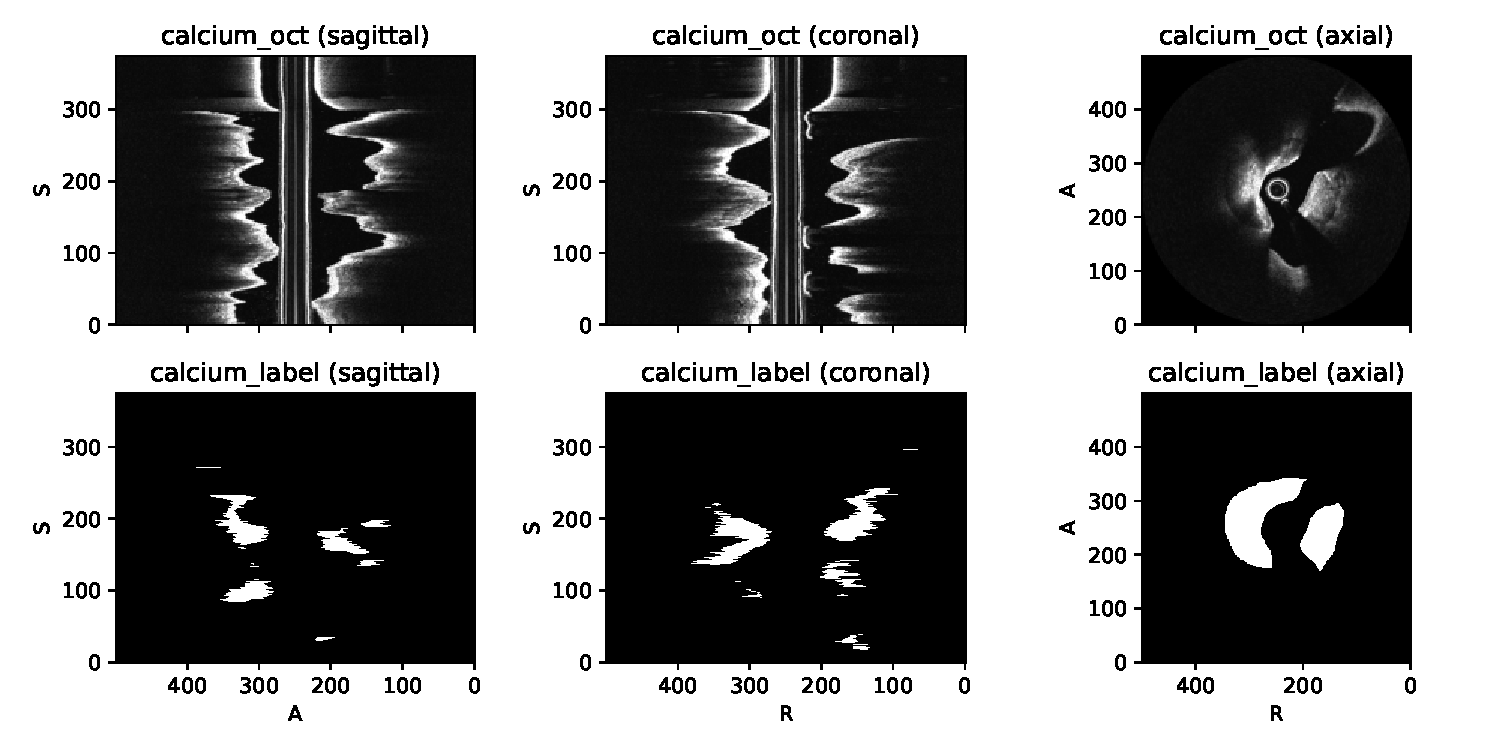
\includegraphics[width=1\linewidth]{figures/fig_datasets_calcium_oct_sample.pdf}
        \caption{An example of an annotated image from the Calcium OCT dataset.}
        \label{fig:calcium-oct}
    \end{subfigure}%
    \hfill
    \begin{subfigure}[t]{0.49\textwidth}
        \centering
        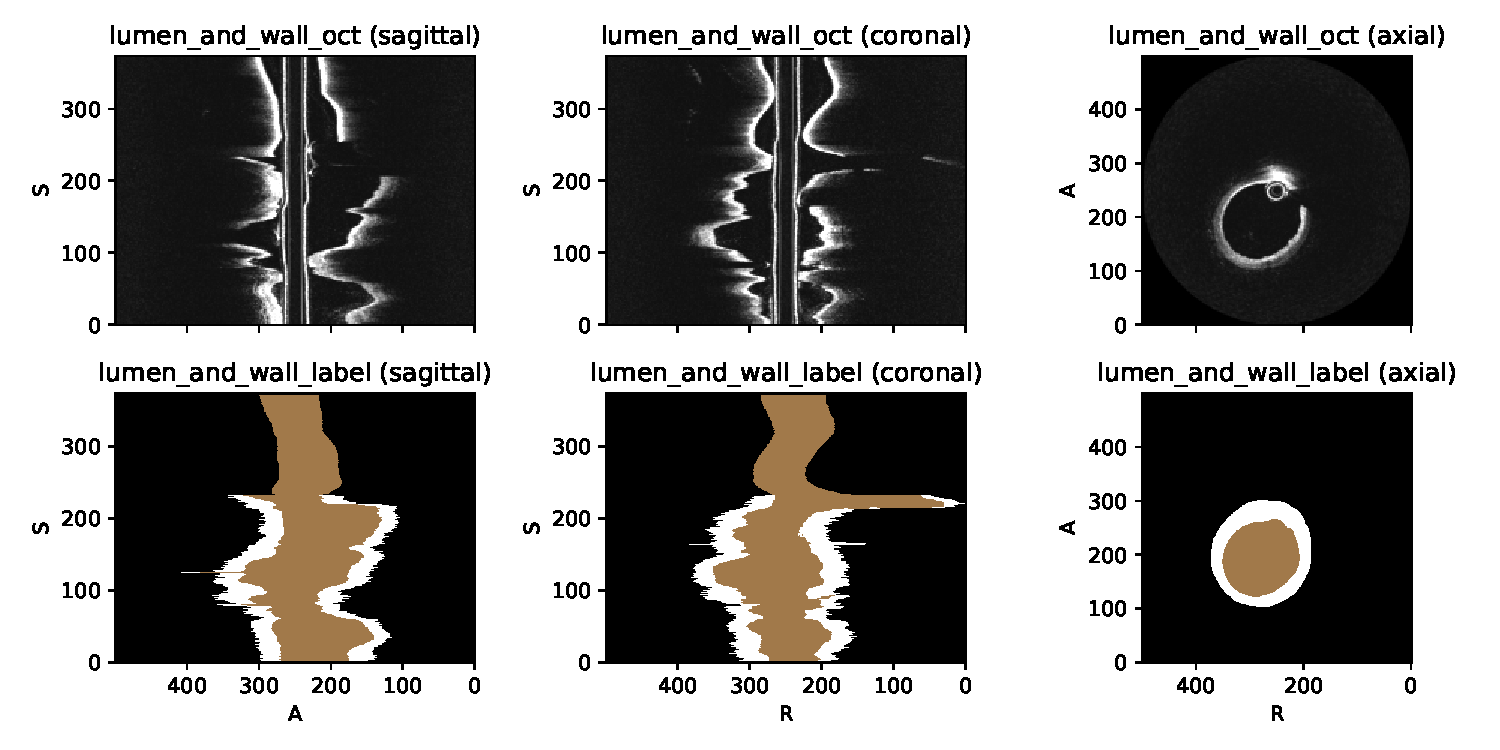
\includegraphics[width=1\linewidth]{figures/fig_datasets_law_oct_sample.pdf}
        \caption{An example of an annotated image from the Lumen and Wall OCT dataset (LaW OCT).}
        \label{fig:lumen-and-wall-oct}
    \end{subfigure}
    \caption{For each image, the top row shows the original image at the middle slice across three axes, while the bottom row displays the corresponding segmentation masks.}
    \label{fig:annotated-oct}
\end{figure}

Each dataset has unique characteristics and is divided into training, validation, and testing sets, except for the unannotated datasets, which are used for self-supervised pre-training.
Calcium OCT has one class, calcium. The size of each image is $500\times 500$ while the depth varies from $375$ to $539$. An example of the annotated image is shown in Figure~\ref{fig:calcium-oct}. The dataset is split into 6 training volumes and 2 testing volumes. The training volumes are divided into 3 folds of training and validation sets. In each fold, the model is trained using the training set, while the best model is selected using the validation set. Subsequently, all models trained on each fold are evaluated on the testing set not seen during training. Finally, the performance of the 3 folds on the testing set can be averaged to report the final performance. This is done to ensure the robust evaluation of the methods.

LaW OCT has 2 classes, lumen, and wall, and is divided into 16 training volumes and 4 testing volumes. The size of each image is $500\times 500$ while the depth varies from $270$ to $540$. An example of the annotated image is shown in Figure~\ref{fig:lumen-and-wall-oct}.

The unannotated datasets are of size $500\times 500$, and varying depth. They are not split into training and testing sets since they are only used for self-supervised pre-training. However, each self-supervised learning algorithm may divided into training and validation sets to track its convergence. Samples of each modality are shown in Figure~\ref{fig:unannotated-oct}.

\begin{figure}[hbt]
    % \centering
    \begin{subfigure}[t]{0.49\textwidth}
        \centering
        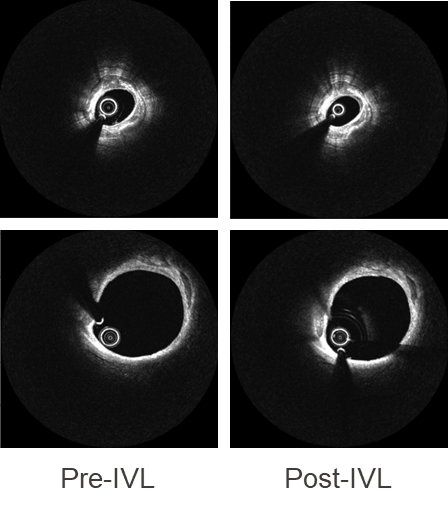
\includegraphics[width=0.65\linewidth]{figures/fig_datasets_coregistered_prepostivl.png}
        \caption{Samples of co-registered images between Pre-IVL and Post-IVL}
        \label{fig:co-registered-oct}
    \end{subfigure}%
    \hfill
    \begin{subfigure}[t]{0.49\textwidth}
        \centering
        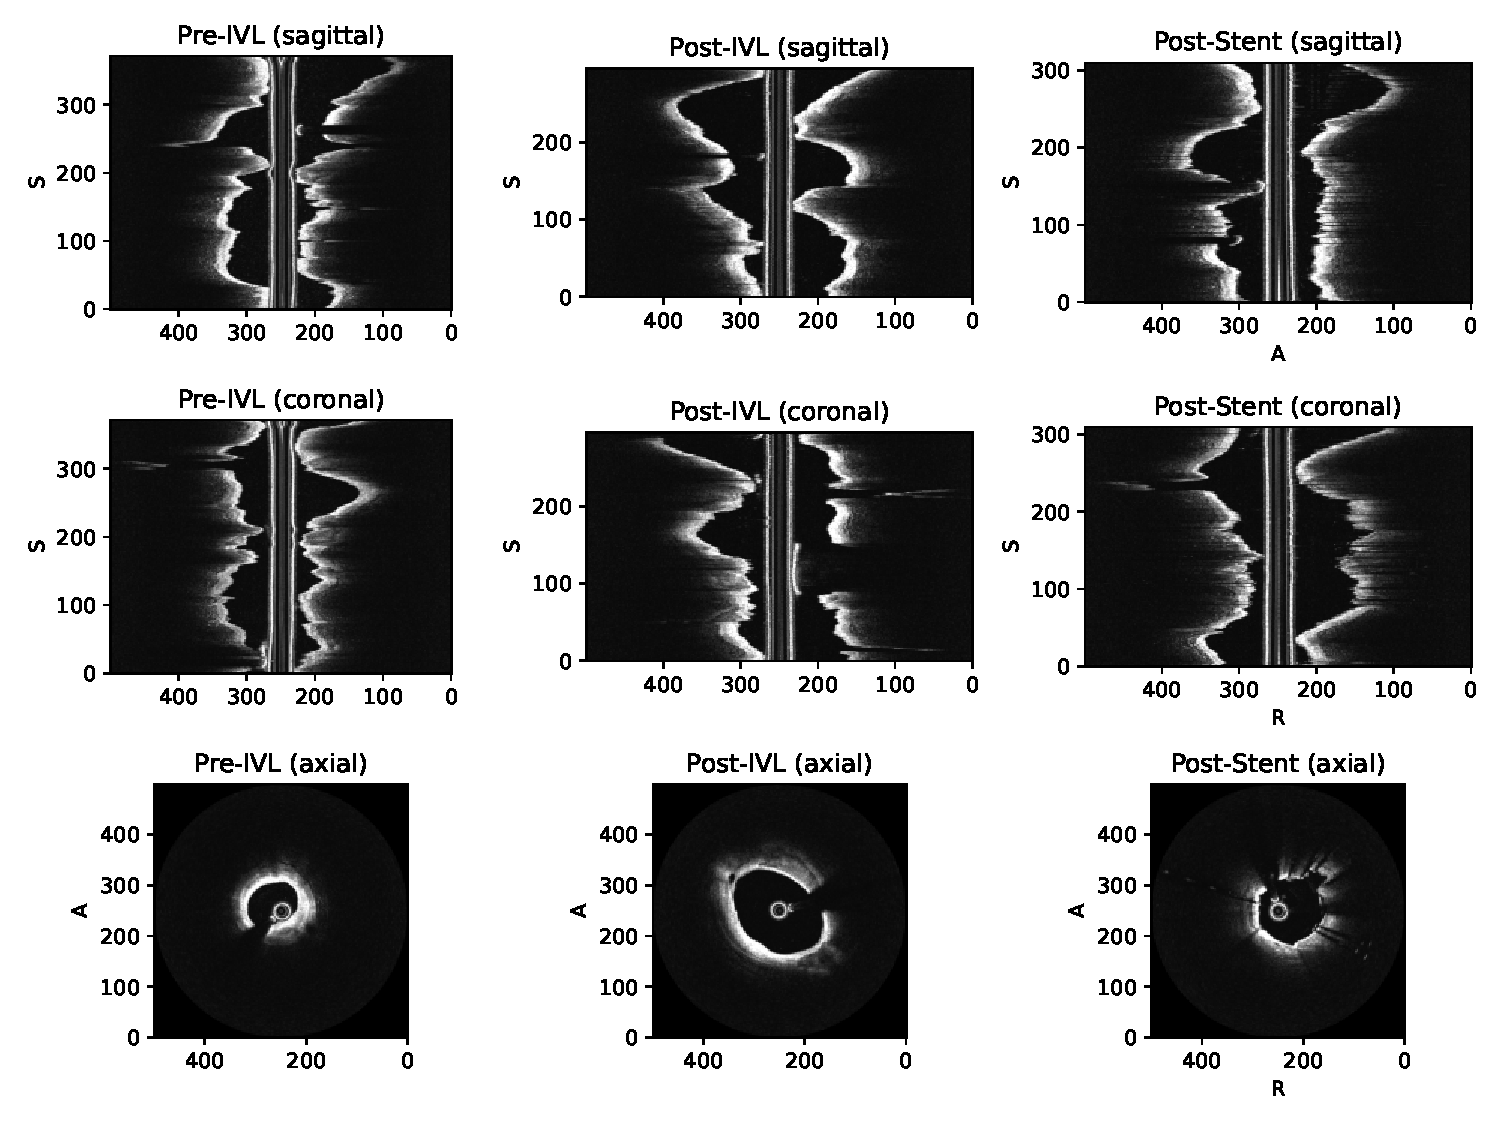
\includegraphics[width=1\linewidth]{figures/fig_datasets_unlabeled_oct_sample.pdf}
        \caption{Samples of unannotated OCT images: the left column shows Pre-IVL, the middle column Post-IVL, and the right column Post-Stent OCT.}
        \label{fig:unannotated-oct}
    \end{subfigure}
    \caption{For each image, the top row shows the original image at the middle slice across three axes, while the bottom row displays the corresponding segmentation masks.}
\end{figure}

\newpage
\section{Algorithms}
In this section, we describe various learning methods for calcium segmentation, categorizing them into supervised and self-supervised approaches. Supervised learning involves either training a model from scratch using only the Calcium OCT dataset or pre-training it on another annotated dataset before fine-tuning it for calcium segmentation. This pre-training on annotated dataset is referred to as supervised pre-training, while the subsequent fine-tuning is known as transfer learning. In contrast, self-supervised learning involves pre-training a model on an unannotated dataset followed by fine-tuning on the Calcium OCT dataset. The key difference between supervised and self-supervised in this study lies in whether the pre-training process requires human annotation. It is important to note that CLIP is typically categorized as a weakly supervised learning method since it relies on human annotations to co-register pairs of different modalities. However, as we advance towards automatic co-registration, we have opted to classify it under self-supervised learning for simplicity.

\subsection{Supervised Learning}
\subsubsection{nnUNet}\label{sec:design:nnunet}
nnUNet is a self-configuring framework for medical image segmentation~\cite{Isensee2020}. First, the data fingerprint must be provided to nnUNet, which specifies the number of image modalities, normalization process for each modality, and the number of segmentation classes. Additional details, such as intensity range, image spacing, shape, and resolution, are derived from the metadata. Using this fingerprint, nnUNet automatically determines the network topology, sampling strategy, data augmentation approach, batch size, and patch size for the training process. Notably, nnUNet also offers a supervised pre-training pipeline, allowing the model to be trained on other datasets before fine-tuned on the target dataset.

We designed two approaches to apply the algorithm to our datasets. The first approach involves directly training the model on the Calcium OCT dataset. In the second approach, we pre-trained the model on the LaW OCT dataset before fine-tuning it for calcium segmentation. 

nnUNet offers both 2D and 3D segmentation architectures, as well as a cascade 3D architecture combining full-resolution and low-resolution networks. Our preliminary experiments indicated that the 2D and 3D architectures outperformed the cascade architecture. Consequently, we decided to use only the 2D and 3D architectures for the remainder of our experiments.

\subsubsection{SegFormer}
SegFormer is a transformer-based model that integrates multi-resolution feature fusion through simple multi-layer perceptrons (MLP~\cite{Rumelhart1986})~\cite{Xie2021SegFormer}. Pre-trained on the ADE20k dataset~\cite{Zhou2018}, SegFormer mirrors U-Net's encoder by downsampling input images via overlap patch merging, which unifies adjacent patches into a single unit. This process allows the model to capture the features at various resolutions. Furthermore, SegFormer utilizes these multi-resolution features with an All-MLP decoder, which aligns lower-resolution features with the channels of their higher-resolution counterparts. The decoder then upsamples the features up to the original resolution and concatenates them with the higher-resolution features, ultimately predicting the segmentation masks using only MLPs and upsampling layers. 

SegFormer architectures comes in various sizes, from MiT-B1 to MiT-B5, with the largest model, MiT-B5, containing 84.7M parameters. We fine-tuned the largest pre-trained model on Calcium OCT for 80,000 iterations, which was sufficient for the model to converge.

\subsubsection{RADIO}
RADIO is a distillation framework that enables the use of multiple vision foundational models as teachers \cite{Ranzinger2024RADIO}. The framework was assessed on 2D segmentation tasks, incorporating batch normalization and linear projection in the decoder head. In alignment with this evaluation protocol, we employed their pre-trained ViT model. Specifically, we utilized the RADIO ViT-H/16 model and fine-tuned it on the Calcium OCT dataset. The training was conducted for 80,000 iterations, which was determined to be adequate for model convergence.

\subsubsection{SuPreM}~\label{sec:design:suprem}
SuPreM is a supervised pre-training method specifically designed for 3D medical image segmentation \cite{Li2024}. It involves training models on a large scale dataset of CT volumes before fine-tuning. Among the models pre-trained with SuPreM, we chose the SwinUNTER model~\cite{Tang2022} due to its reported superior performance and fine-tuned it on the Calcium OCT dataset. It is important to note that the publicly available models have been pre-trained on 2,100 CT volumes, rather than 9,262, as the authors have not yet released the fully pre-trained versions.

SwinUNTER is a transformer-based model designed for segmenting brain tumors in 3D MRI images. Its architecture is built upon the Swin Transformer encoder, extracting hierarchical features from the input image.~\cite{Liu2021Swin}. The model also includes a CNN-based decoder, UNTER, featuring convolutional layers with upsampling and skip connections to merge features across different levels~\cite{Hatamizadeh2022}. The authors of SwinUNTER proposed a self-supervised learning algorithm for the model~\cite{Tang2022}. 

To evaluate the algorithms, we conducted three experiments. The first experiment fine-tuned the pre-trained model on the Calcium OCT dataset. The second experiment involved fine-tuning the self-supervised SwinUNTER model on the same dataset. The third experiment trained the SwinUNTER model from scratch, serving as a baseline to assess the effectiveness of SuPreM pre-training and the self-supervised learning method proposed for SwinUNTER within the context of the Calcium OCT dataset.

\subsection{Self-Supervised Learning}
\subsubsection{V-JEPA}
V-JEPA is a self-supervised learning method that learns representations by predicting the masked parts of a video. It uses a context encoder to make these predictions and compares the predicted latent vectors with those generated by a target encoder, which views the video without masking~\cite{Bardes2024Vjepa}. The author provides ViT models pre-trained on the VideoMix2M dataset, which contains 2 million videos, using V-JEPA pre-training. We conducted two experiments to evaluate the effectiveness of V-JEPA on OCT images. First, we fine-tuned the V-JEPA model on Calcium OCT. In the second experiment, we applied V-JEPA pre-training to the Unannotated OCT (Dataset ~\ref{enum:unannotated-dataset}) and fine-tuned the resulting model on Calcium OCT. Since the original paper does not address segmentation tasks, we will discuss the implementation of the decoder head in Section~\ref{sec:implementation:vjepa}.

\subsubsection{Genesis}
Genesis is a self-supervised learning method that learns representations by restoring the original images from their corrupted versions~\cite{Zhou2021}. In their paper, Genesis is applied to a U-Net architecture, which contains 15M parameters. We adapted their method to the same 3D nnUNet architecture in Section~\ref{sec:design:nnunet}, which has 30M parameters. Thereafter, we applied Genesis pre-training to unannotated OCT images and fine-tune the resulting model on Calcium OCT.

\subsubsection{CLIP}
Contrastive Language-Image Pre-training (CLIP) is a contrastive learning method that matches encoded vectors of images with their text captions~\cite{Radford2021CLIP}. In our work, we adapted CLIP to OCT images by using co-registered Pre-IVL and Post-IVL images. We used the same nnUNet architecture as described in Section~\ref{sec:design:nnunet}. CLIP pre-training was applied to the 3D nnUNet which was was then fine-tuned on the Calcium OCT dataset. To implement this, we modified code from a publicly available project~\cite{Shariatnia2021}. While the original paper proposed a pre-training framework for aligning language and images, we tailored this framework for use with co-registered OCT images. Details of this adaptation will be discussed in Section~\ref{sec:implementation:clip}.

%%%%%%%%%%%%%%%%%%%%%%%%
\chapter{Implementation}
%%%%%%%%%%%%%%%%%%%%%%%%

% The implementation covers some of the implementation details of your project.
% This is not intended to be a low-level description of every line of code that
% you wrote but covers the implementation aspects of the projects.

% This section is usually 3-5 pages.
\section{Supervised Learning}
\subsubsection{nnUNet}
We applied the official nnUNet~\cite{Isensee2020} code on our datasets, adding an early stopping criterion to the optimizer. In particular, we observed that the 3D segmentation performance of nnUNet was significantly worse than its 2D counterpart. To address this, we experimented with different patch sizes for 3D segmentation, diverging from the default settings. Reducing the depth of the original patch size from $112$ to $32$ improved performance significantly. This could be because smaller depth provided the model with more examples to learn from. In the second experiment, we pre-trained the model on LaW OCT before fine-tuning it on Calcium OCT using the supervised pre-training script provided by nnUNet.

\subsubsection{SegFormer}\label{sec:implementation:segformer}
We adopted the pre-trained SegFormer model along with a training script from MMSegmentation~\cite{mmseg2020}. Since SegFormer is designed exclusively for 2D segmentation, we pre-processed our Calcium OCT dataset into 2D images before training the model on the reformatted data. To ensure a fair comparison, we also maintained the same three folds and testing set as those used in nnUNet.

\subsubsection{RADIO}
We utilized the pre-trained RADIO's ViT model and its training script available in MMSegmentation~\cite{mmseg2020}. Since RADIO, like SegFormer, only supports 2D segmentation, we used the same pre-processed datasets as described in Section~\ref{sec:implementation:segformer}.

\subsubsection{SuPreM}
SuPreM provides official pre-trained models and code~\cite{Li2024}. Accordingly, we reformatted our Calcium OCT dataset to align with the format of SuPreM's datasets, while ensuring that the three folds and testing set remained consistent with those used in other experiments within this study. We three experiments, as outlined in Section~\ref{sec:design:suprem}, employing the official script from SuPreM.

\section{Self-Supervised Learning}
\subsubsection{V-JEPA}\label{sec:implementation:vjepa}
We developed three segmentation decoder heads for the Vision Transformer (ViT) pre-trained with V-JEPA, because it had previously been evaluated solely on classification tasks using an encoder-only transformer referred to as attentive decoder. To extend its utility to segmentation tasks, we designed an attentive decoder head for segmentation, drawing inspiration from the MAE decoder~\cite{He2022}, which directly predicts pixel values. Specifically, our decoder head employs an encoder-only transformer of 1 depth and 12 attention heads, followed by a linear projection layer that transforms embedding vectors into a vector of size \(\{\text{patch size} \times \text{patch size} \times \text{number of classes}\}\). 

In addition, we experimented with alternative decoding architectures, such as a simple batch normalization layer followed by a linear projection, similar to the adaptations made in RADIO~\cite{Ranzinger2024RADIO} and DINOv2~\cite{Oquab2024dinov} for segmentation tasks. Both variations are illustrated in Figure~\ref{fig:vjepa-attentive-and-batchnorm-decoder-head}. 

\begin{figure}[ht]
    \centering
    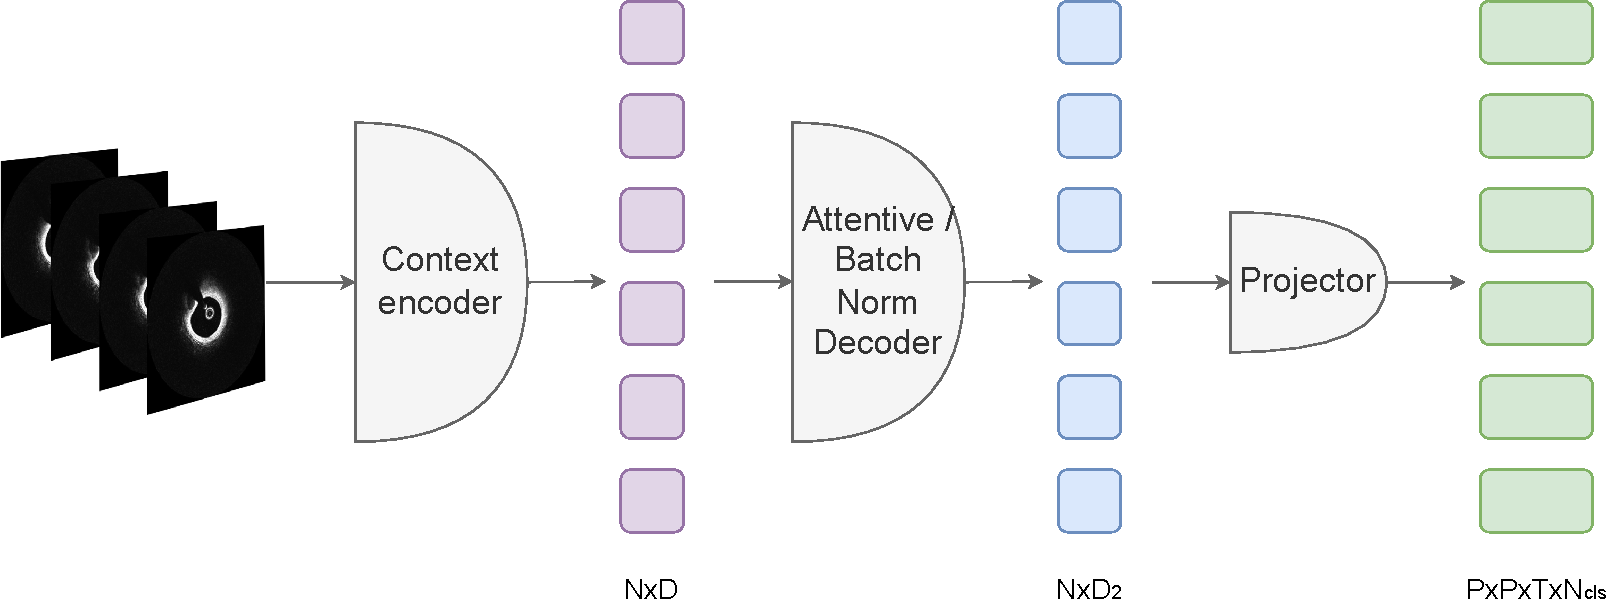
\includegraphics[width=0.6\linewidth]{figures/fig_implementation_vjepa_attentive_and_batchnorm_decoder.pdf}
    \caption{Attentive and linear batch normalization decoder head for ViT (V-JEPA).}
    \label{fig:vjepa-attentive-and-batchnorm-decoder-head}
\end{figure}%

Further, inspired by SegFormer~\cite{Xie2021SegFormer}, we developed multi-feature decoder with a multi-layer perceptron (MLP) on each feature vector at different depths, followed by a linear projection to combine those features into a segmentation mask. This approach allows the decoder to leverage multiple features at various levels. However, unlike SegFormer, our method does not downsample each feature, thereby not explicitly forcing them to lower resolutions. Ultimately, this method allowed us to utilize ViT pre-trained with V-JEPA, ViT (V-JEPA), in our segmentation task. The multi-feature decoder head is shown in Figure~\ref{fig:vjepa-multi-feature-decoder-head}.

\begin{figure}[ht]
    \centering
    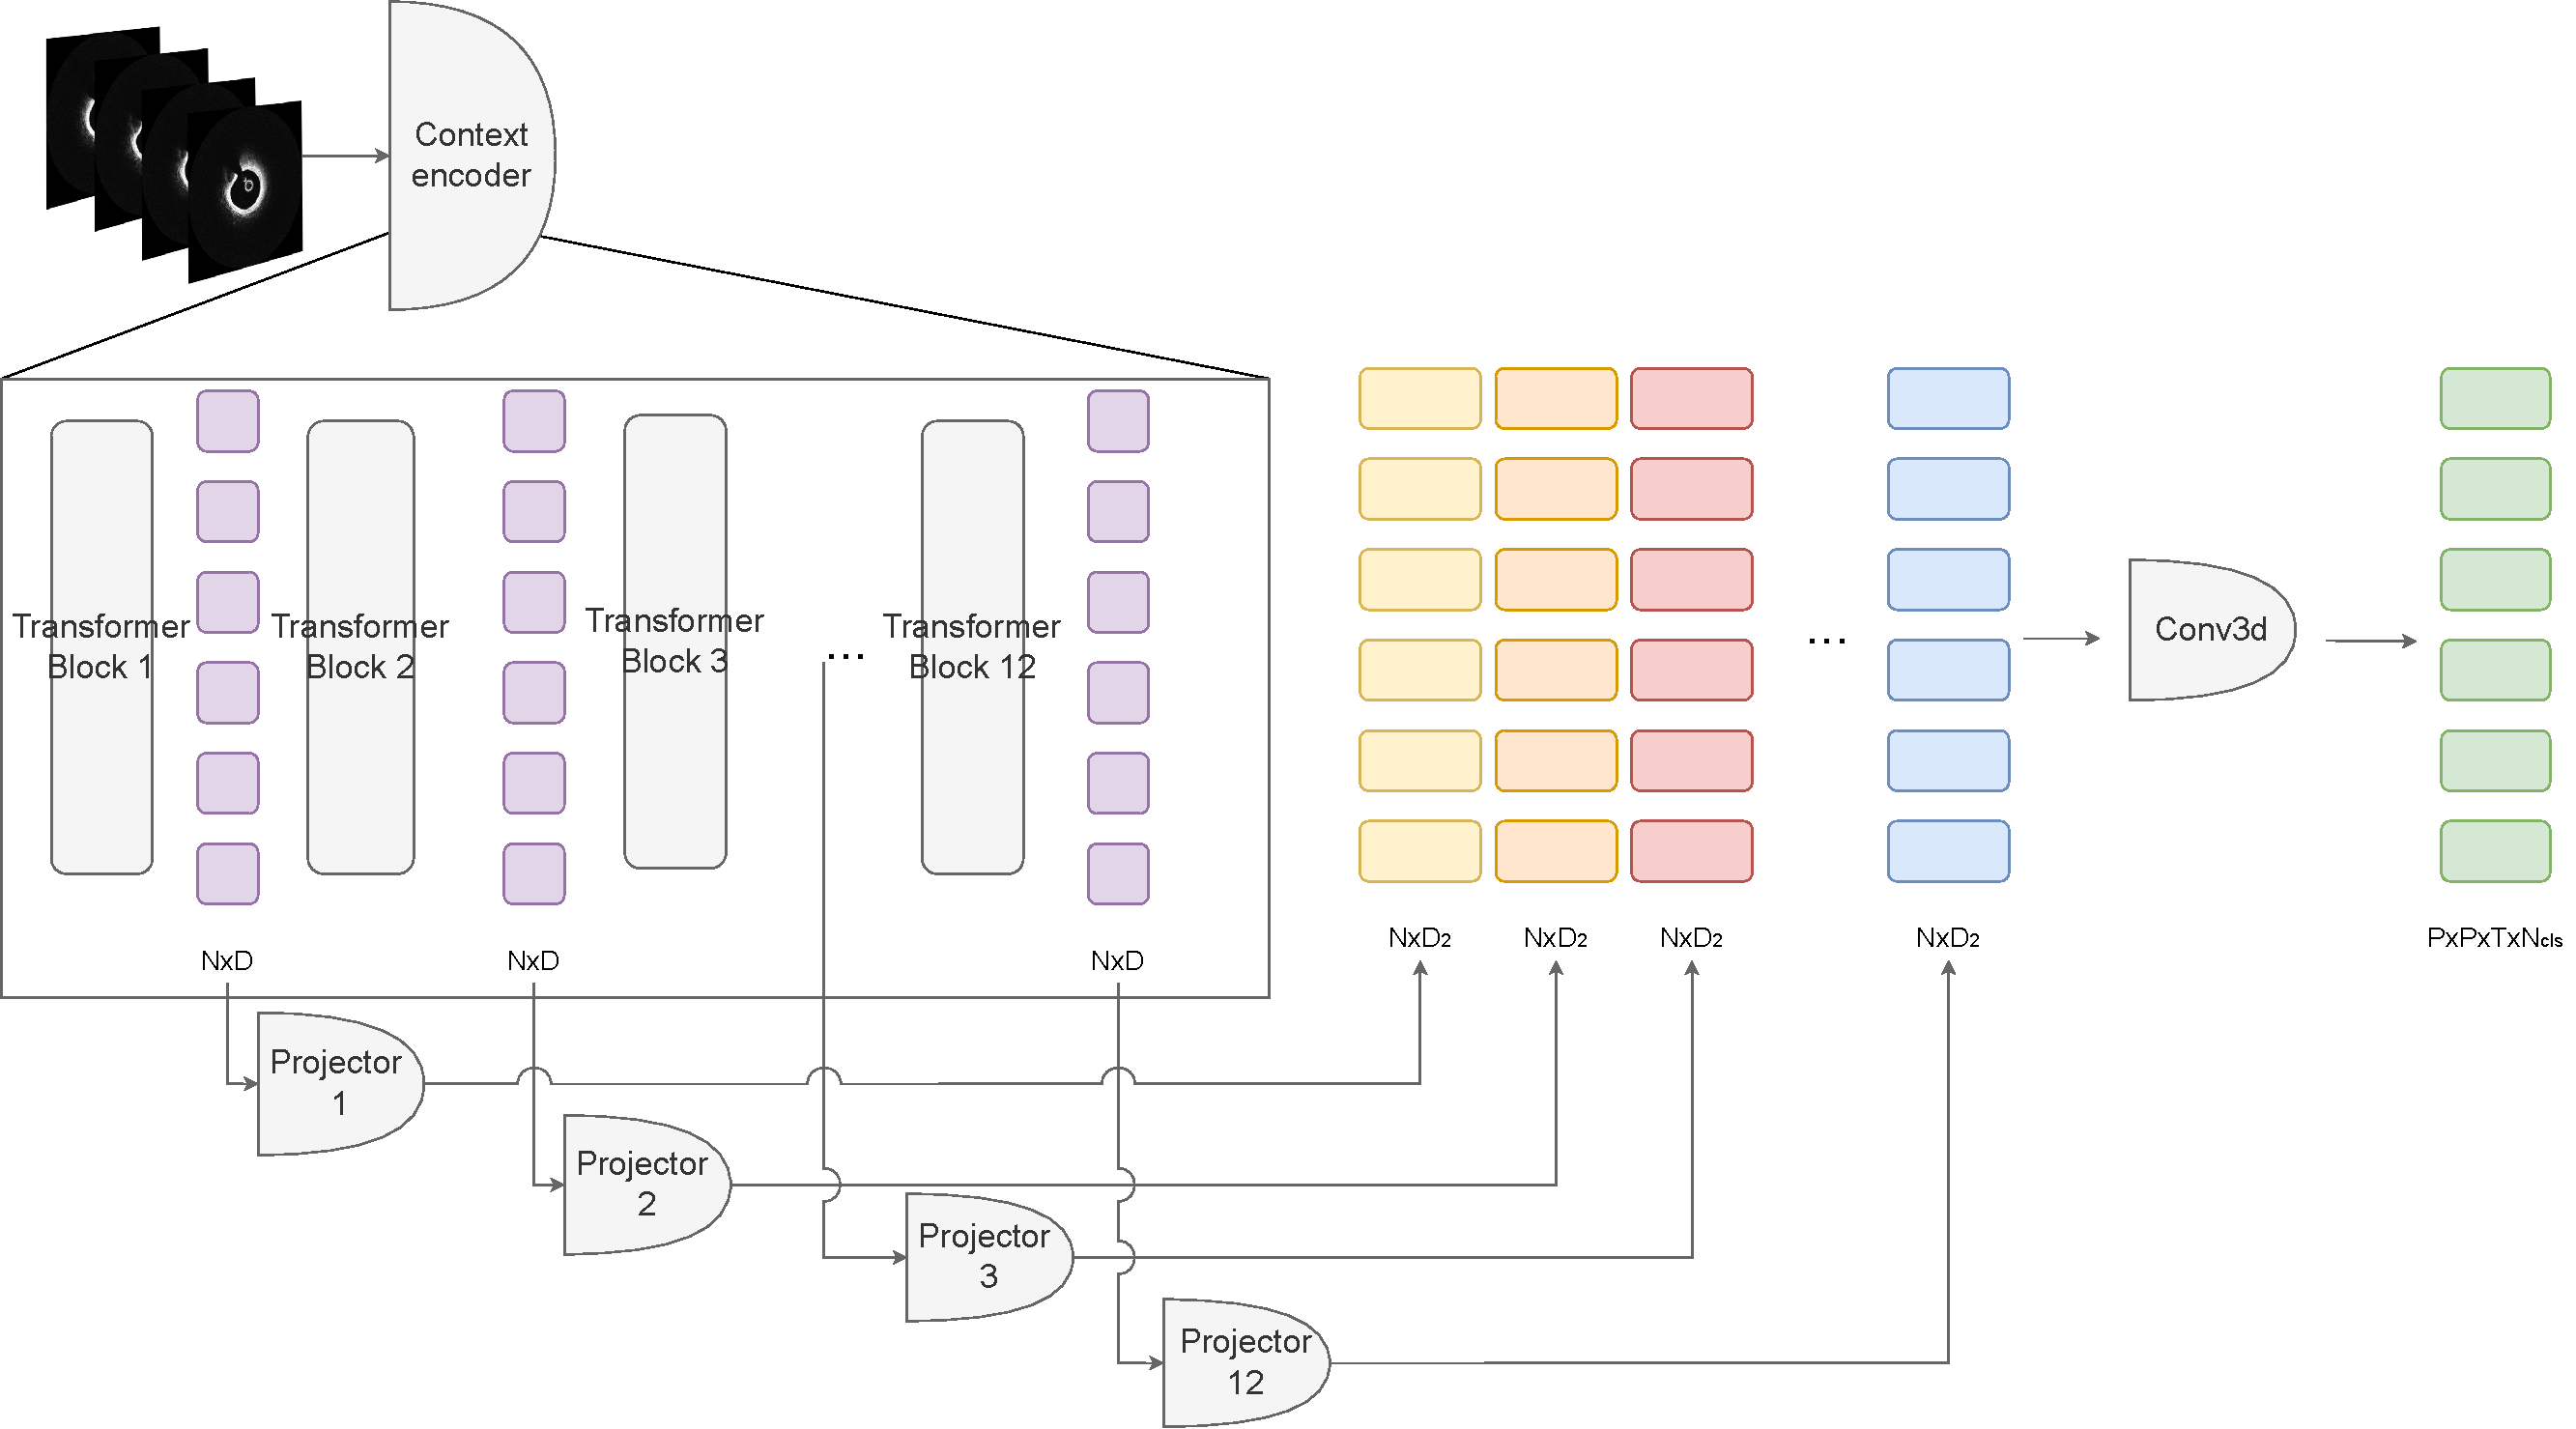
\includegraphics[width=1.0\linewidth]{figures/fig_implementation_vjepa_multifeat.pdf}
    \caption{A multi-feature decoder head. Feature at each transformer block is projected to the same dimension and concatenated before being passed to a convolutional layer that produces the segmentation mask.}
    \label{fig:vjepa-multi-feature-decoder-head}
\end{figure}

\subsubsection{Genesis}
We altered the official code for Genesis provided by the authors~\cite{Zhou2021} by adding a pre-processing step to the method. Genesis implementation begins with an initial pre-processing step on unannotated OCT images, where small cubes of size $64\times 64\times 64\times 32$ are sampled from the volumes. These cubes are then dynamically corrupted during the Genesis pre-training process. The authors recommend sampling $96$ cubes per volume, noting that increasing this number does not necessarily improve the performance and adds computation cost. Following this recommendation, we implemented an additional sampling strategy to enhance the quality of the cubes.

Our strategy involved randomly sampling $96$ cubes from each volume, ensuring that the selected cubes contained enough information, given that OCT images often contain substantial background, unlike CT images used in the original paper. We achieved this by applying a thresholding technique, selecting only those cubes with average intensities above a certain threshold. As illustrated in Figure~\ref{fig:genesis-cubes-with-threshold}, the resulting cubes contain meaningful structures such as the artery's lumen and wall. In contrast, without our thresholding strategy, the sampled cubes are dominated by background noise, as shown in Figure~\ref{fig:genesis-cubes-without-threshold}. We trained the model on these cubes until convergence.

\begin{figure}[t]
    \centering
    \begin{subfigure}{0.48\textwidth}
        \centering
        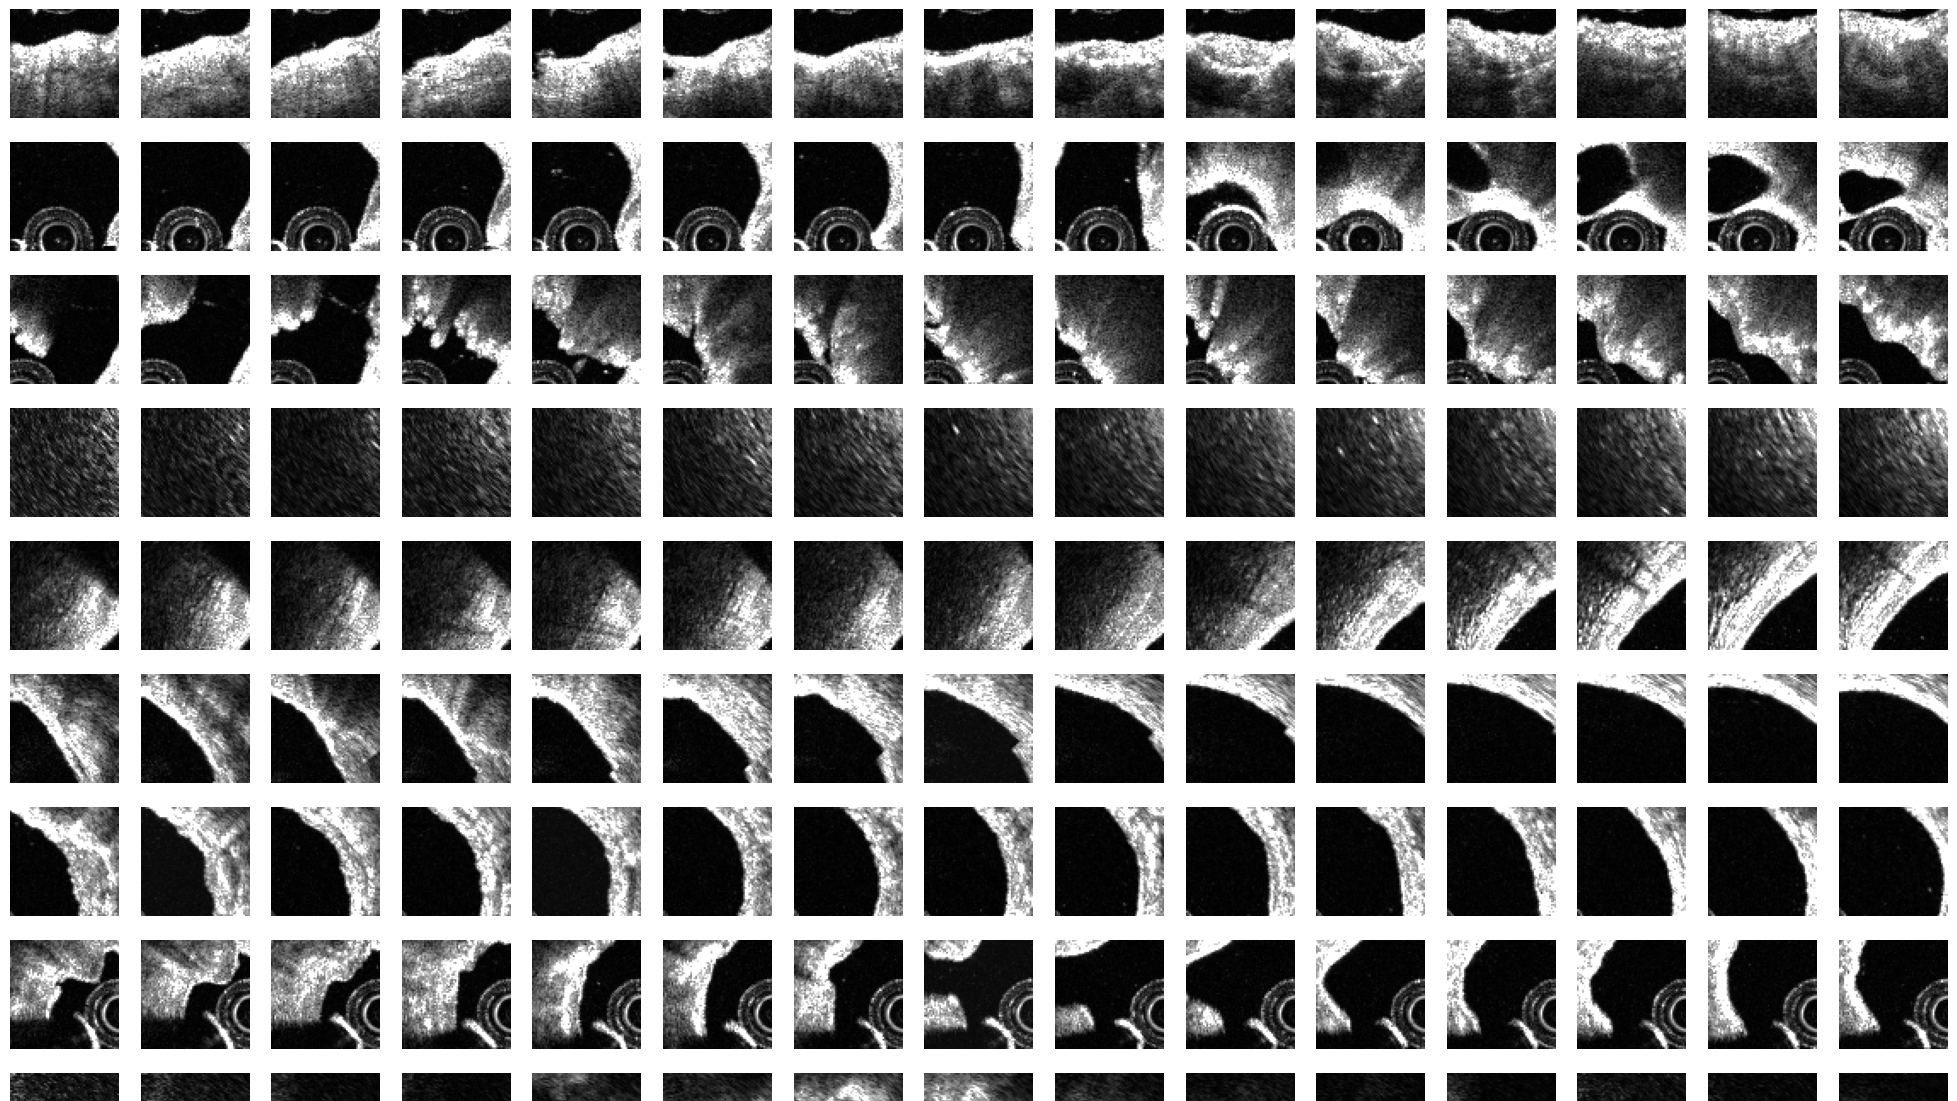
\includegraphics[width=0.9\linewidth]{figures/fig_implementation_genesis_extracted_cube.png}
        \caption{Cubes from unannotated OCT images sampled with the thresholding strategy.}
        \label{fig:genesis-cubes-with-threshold}

    \end{subfigure}%
    \hfill
    \begin{subfigure}{0.48\textwidth}
        \centering
        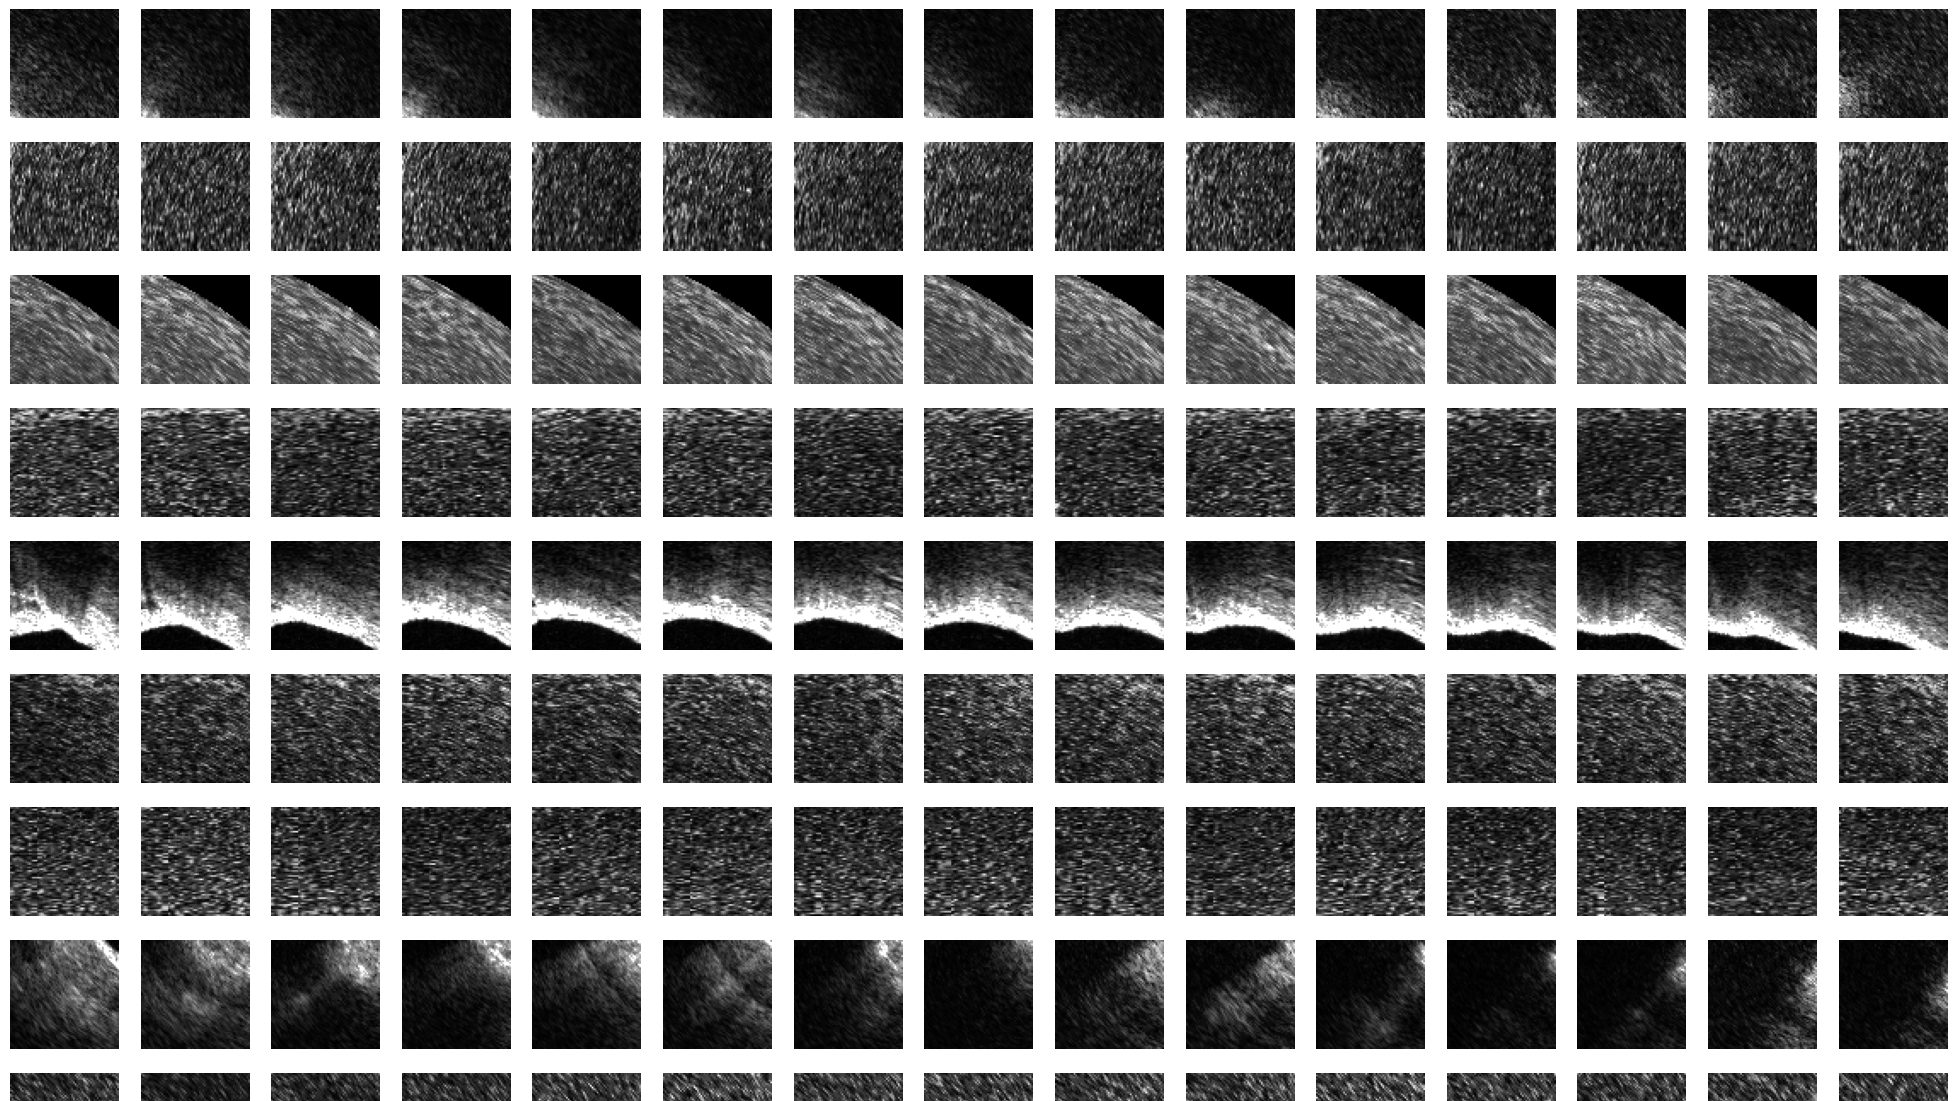
\includegraphics[width=0.9\linewidth]{figures/fig_implementation_genesis_extracted_cube_no_threshold.png}
        \caption{Examples of cubes sampled from unannotated OCT images. Each row represents a sampled cube with slices unrolled along the depth dimension.}
        \label{fig:genesis-cubes-without-threshold}
    \end{subfigure}
    \caption{Samples of cubes from unannotated OCT images. Each row is a sampled cube with slices unrolled along the depth dimension.}
\end{figure}

For fine-tuning, we loaded the pre-trained weights of the model's encoder and decoder into the 3D nnUNet, leaving the segmentation head to be randomly initialized. We then fine-tuned the pre-trained model on the Calcium OCT dataset, utilizing the optimal patch size of $160\times 128\times 32$ (height by width by depth) identified in Section~\ref{sec:result:nnunet}. The nnUNet's training script was used with the same configurations as the supervised pre-training, providing the pre-trained model as the initial weights.

\subsubsection{CLIP}\label{sec:implementation:clip}
We adopted the CLIP model, originally designed for language-image pairs, to work with paired Pre-IVL and Post-IVL volumes by replacing the text encoder with an image encoder. However, this straightforward modification did not result in successful pre-training convergence, necessitating further adjustments using a shared encoder.

Our experiments revealed that using separate encoders and projectors for each modality was less effective than employing a shared encoder and projector. To validate this, we conducted a sanity check by evaluating different encoder and projector configurations. Specifically, we passed the same images through these configurations to see if they could learn to represent the same image as the same vector. We tested three setups: (1) separate encoders and projectors, (2) separate encoders with shared projectors, and (3) shared encoders and projectors. The results showed that the configurations with shared components—either shared projectors or shared encoders and projectors—could match the same image.

Building on these findings, we applied the two successful configurations to the main task of matching co-registered images. Only the configuration with shared encoders and projectors achieved convergence, which is logical as this setup forces the image encoder and projector to learn a representation applicable to both modalities. This process is illustrated in Figure~\ref{fig:clip-oct}. Further details of the experiment are provided in Section~\ref{sec:results:discussion:clip}.

\begin{figure}[hb]
    \centering
    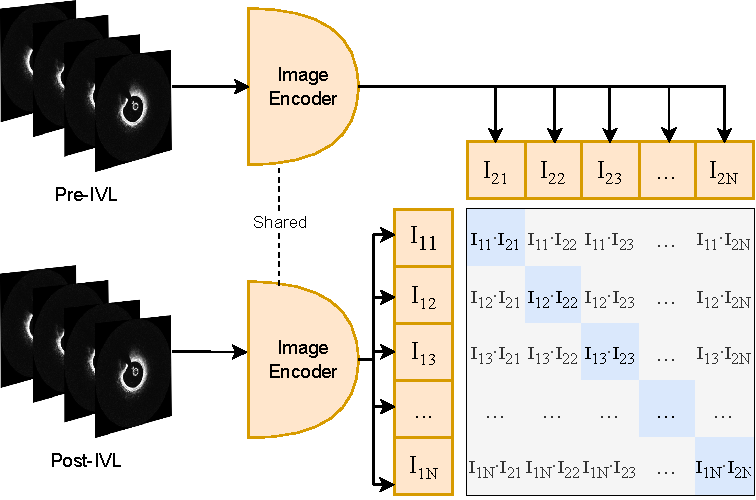
\includegraphics[width=0.65\linewidth]{figures/fig_implementation_clip_oct.pdf}
    \caption{A modified CLIP model for co-registered multi-modal OCT images. Note that the projector is omitted for simplicity. The image encoder and projector are shared across all modalities.}
    \label{fig:clip-oct}
\end{figure}

%%%%%%%%%%%%%%%%%%%%
\chapter{Results and Discussion}
%%%%%%%%%%%%%%%%%%%%

% In the evaluation you convince the reader that your design works as intended.
% Describe the evaluation setup, the designed experiments, and how the
% experiments showcase the individual points you want to prove.

% This section is usually 5-10 pages.
We evaluated the effectiveness of self-supervised learning algorithms on calcium segmentation on coronary OCT images. All the models, pre-trained or not, were fine-tuned on the Calcium OCT dataset using the validation set to select the best model. We did this for 3 folds. The models were then evaluated on the testing set. The performance was measured using the Dice score, a common metric for segmentation tasks. It is defined as follows:

\begin{equation}
    \text{Dice} = \frac{2 \times \text{TP}}{2 \times \text{TP} + \text{FP} + \text{FN}}
\end{equation}

where TP, FP, and FN are true positive, false positive, and false negative, respectively. The Dice score ranges from 0 to 1, where 1 indicates perfect segmentation. The Dice score was calculated for each patient in the testing set, and the average Dice score was reported as the final performance of the model for each fold. The final performance is the average of the Dice scores of all folds.

\section{nnUNet}\label{sec:result:nnunet}
The Dice score of the default configuration of 3D nnUNet is significantly lower than that of the 2D nnUNet. By reducing the depth of the patch size of the 3D nnUNet from $112$ to $32$, the performance increases significantly. This could result from the smaller depth allowing the model to have more examples to learn from. In addition, expanding the width and height of the patch size from $160\times 128$ to $512\times 512$ does not improve performance. This may be due to the nature of calcium plaques in OCT images, which are localized. Thus, increasing the context in the width and height dimensions does not provide additional information to the model. The performance of the nnUNet on the Calcium OCT dataset is summarized in Figure~\ref{fig:nnunet-results}.

\begin{figure}[h]
    \centering
    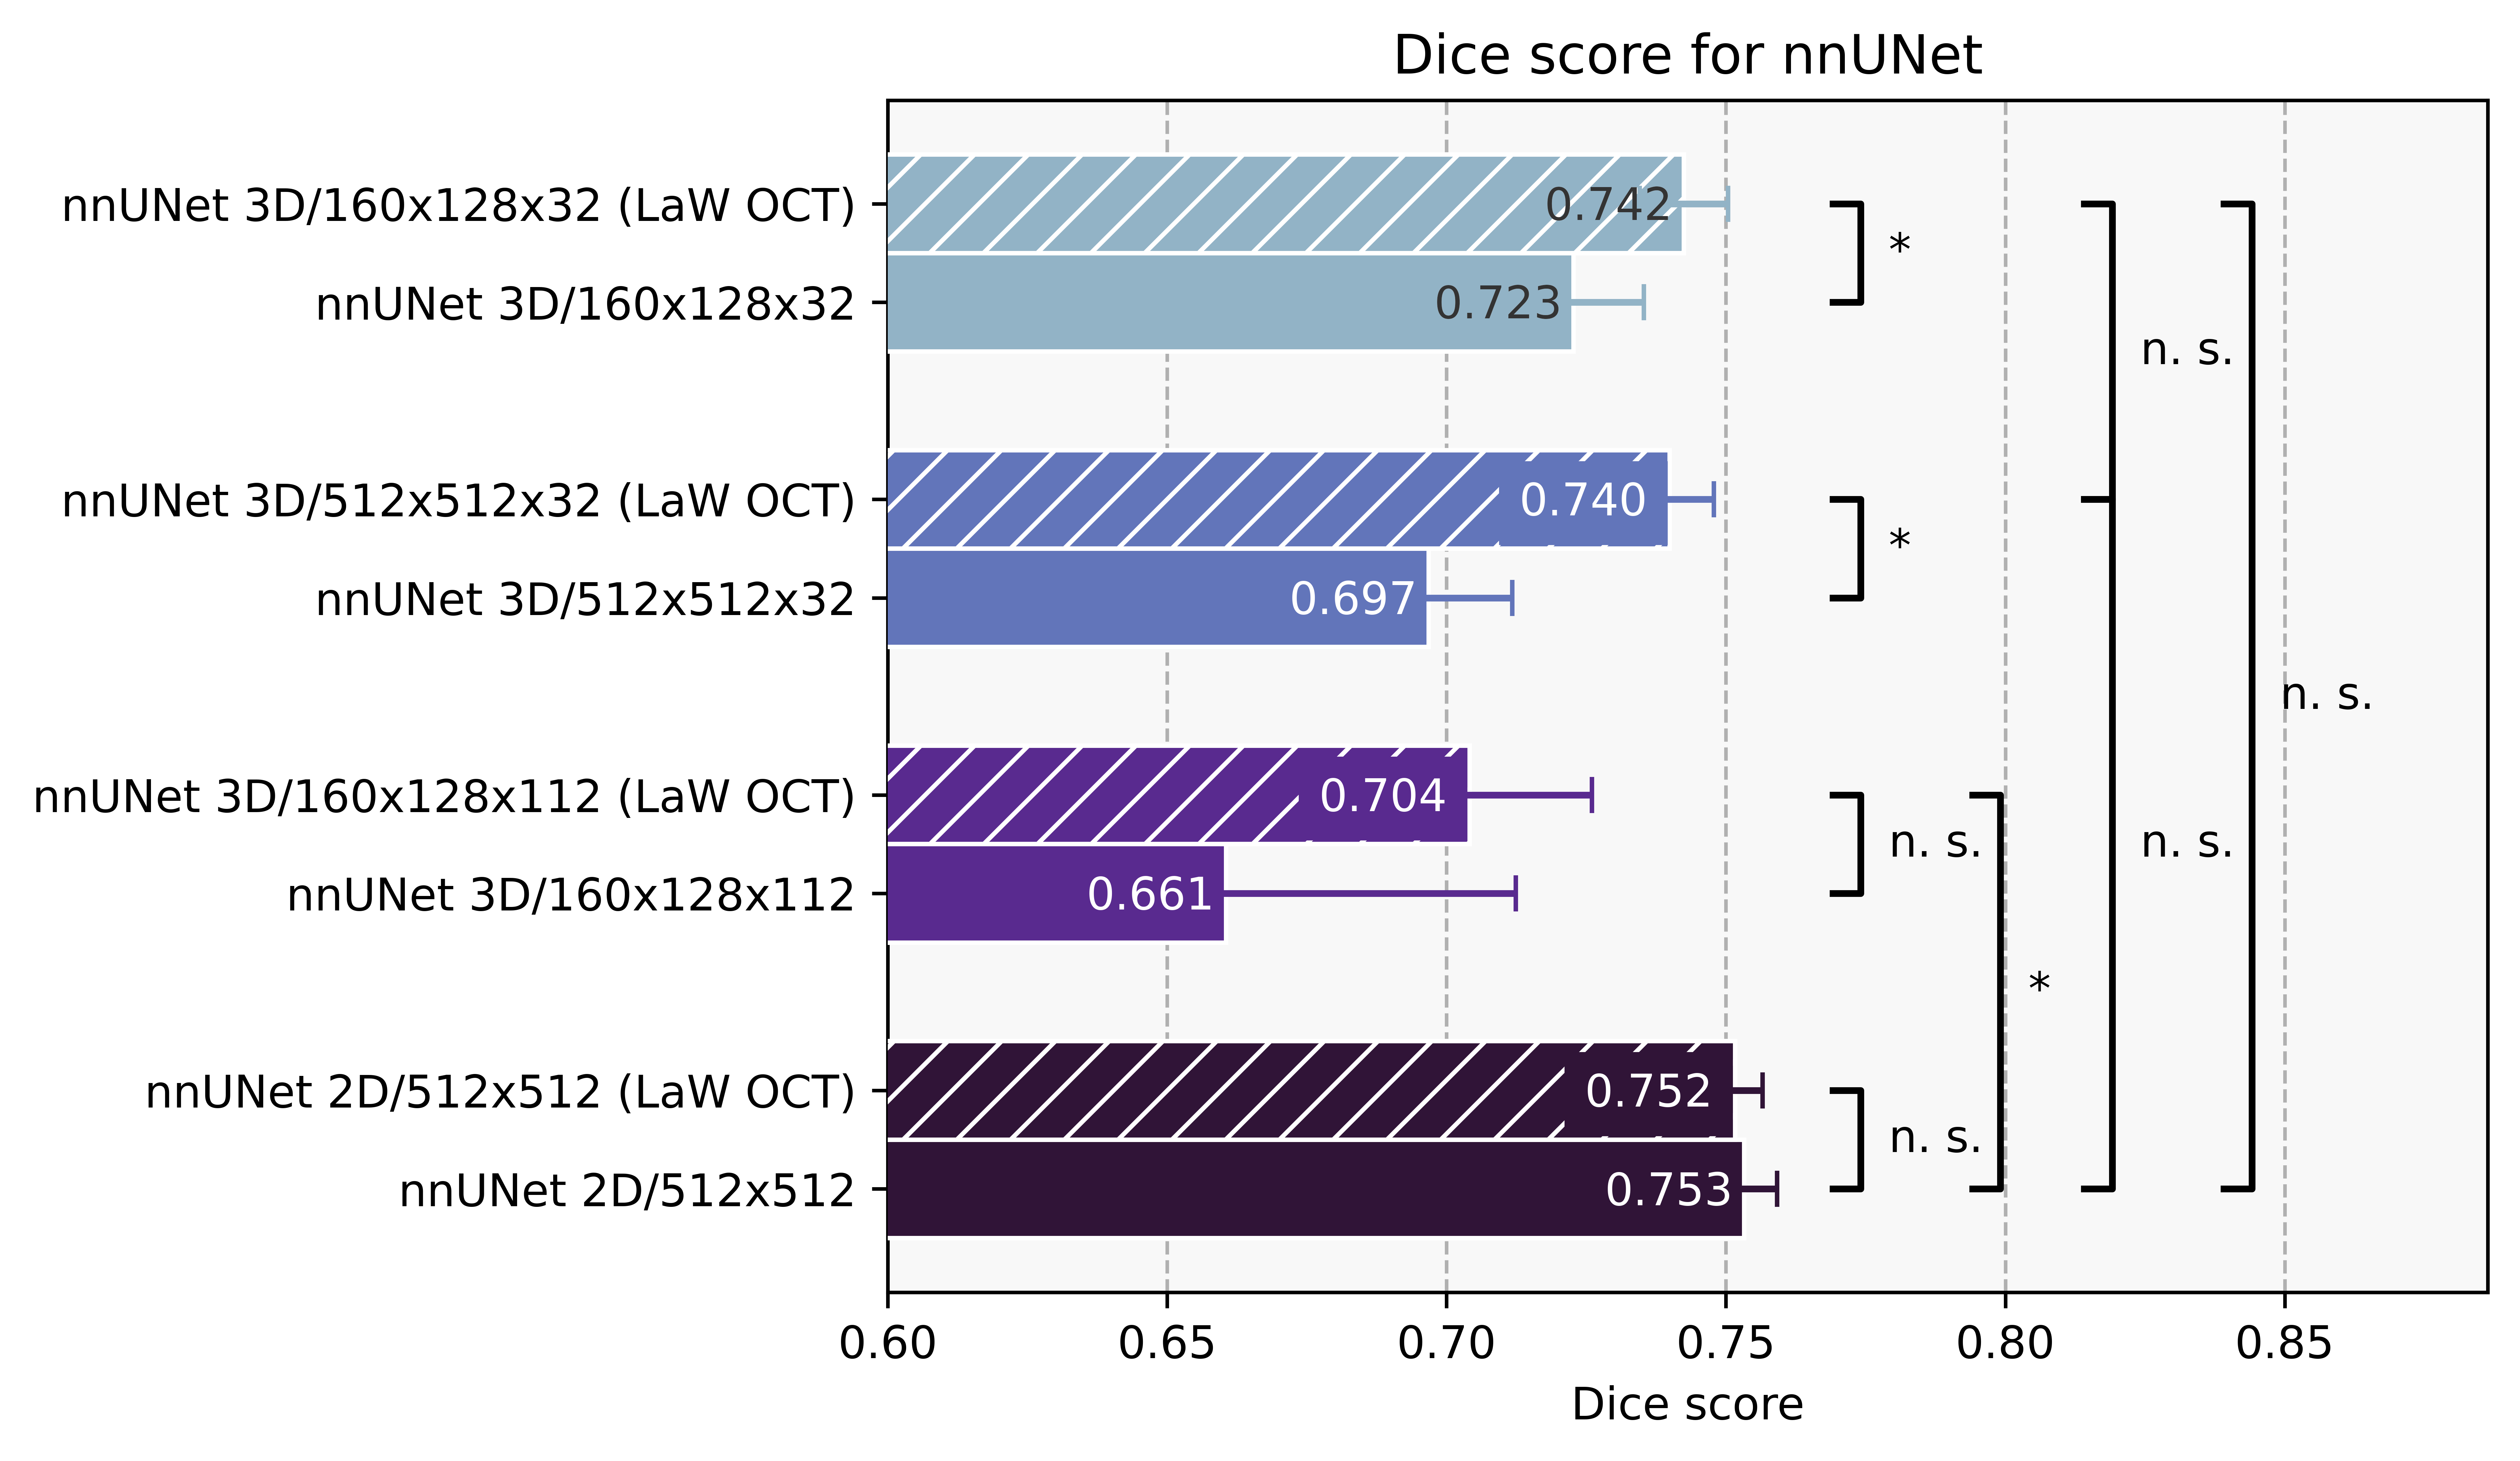
\includegraphics[width=0.8\linewidth]{figures/result_nnunet_results.png}
    \caption{Dice score of variations of nnUNet. Results are grouped according to the patch size used in training. Results in hashes indicate supervised pre-training on the lumen and wall dataset (LaW OCT). 
    % The one-sided paired t-test is done between with and without supervised pre-training. It is also done between the best 2D nnUNet model and the supervised pre-trained 3D nnUNet model. Lastly, the test is done between supervised pre-trained 3D nnUNet models.
    }
    \label{fig:nnunet-results}
\end{figure}

Additionally, pre-training the models with the lumen and wall dataset (LaW OCT) before fine-tuning them on the Calcium OCT significantly improves the 3D performance of the models when their patch sizes are reduced. Calcium plaques are typically located around the periphery of artery walls. Therefore, this pre-training allows the model to learn the features of the walls, which may be useful for calcium segmentation. These pre-trained models are also statistically comparable to the best 2D nnUNet model. As the 2D nnUNet has a better Dice score than the 3D nnUNet, the question arises: Is 3D segmentation necessary, or should we only study 2D segmentation models?

The answer depends on the use cases of the resulting segmentation. In our research, we place greater emphasis on the continuity of the segmentation, as one of the use cases is to reconstruct a 3D digital twin of the image. Consequently, we analyzed the correctness and consistency of the 2D and 3D nnUNet. To add more variety to the consistency analysis, we examined the validation images of each fold rather than the testing images. First, we defined continuity to be the inverse of changes between adjacent segmentation slices. The mathematical definition is as follows.

\begin{equation}
\text{Continuity} = \left(\frac{1}{M\times (N - 1)}\sum_{i = 1}^{M}\sum_{j = 1}^{N-1} \left| I_{j}^{i} - I_{j+1}^{i}\right|\right)^{-1}
\end{equation}

where $M$ is the number of validation images and $N$ is the number of slices per volume. $I_{j}^{i}$ denotes a segmentation mask of the $j$th slice at the $i$th volume. Using this definition, we tracked the Dice scores of the validation images while progressively applying morphological operations -- first opening and then closing -- to enhance segmentation continuity. To enhance continuity, we applied different kernel shapes and sizes. The kernels included 3D spheres and ellipsoids. In ellipsoids, the semi-axis in the depth dimension is greater than the others, as discontinuity was likely to occur. The result is illustrated in Figure~\ref{fig:nnunet-continuity-vs-correctness}.

\begin{figure}[htb]
    \centering
    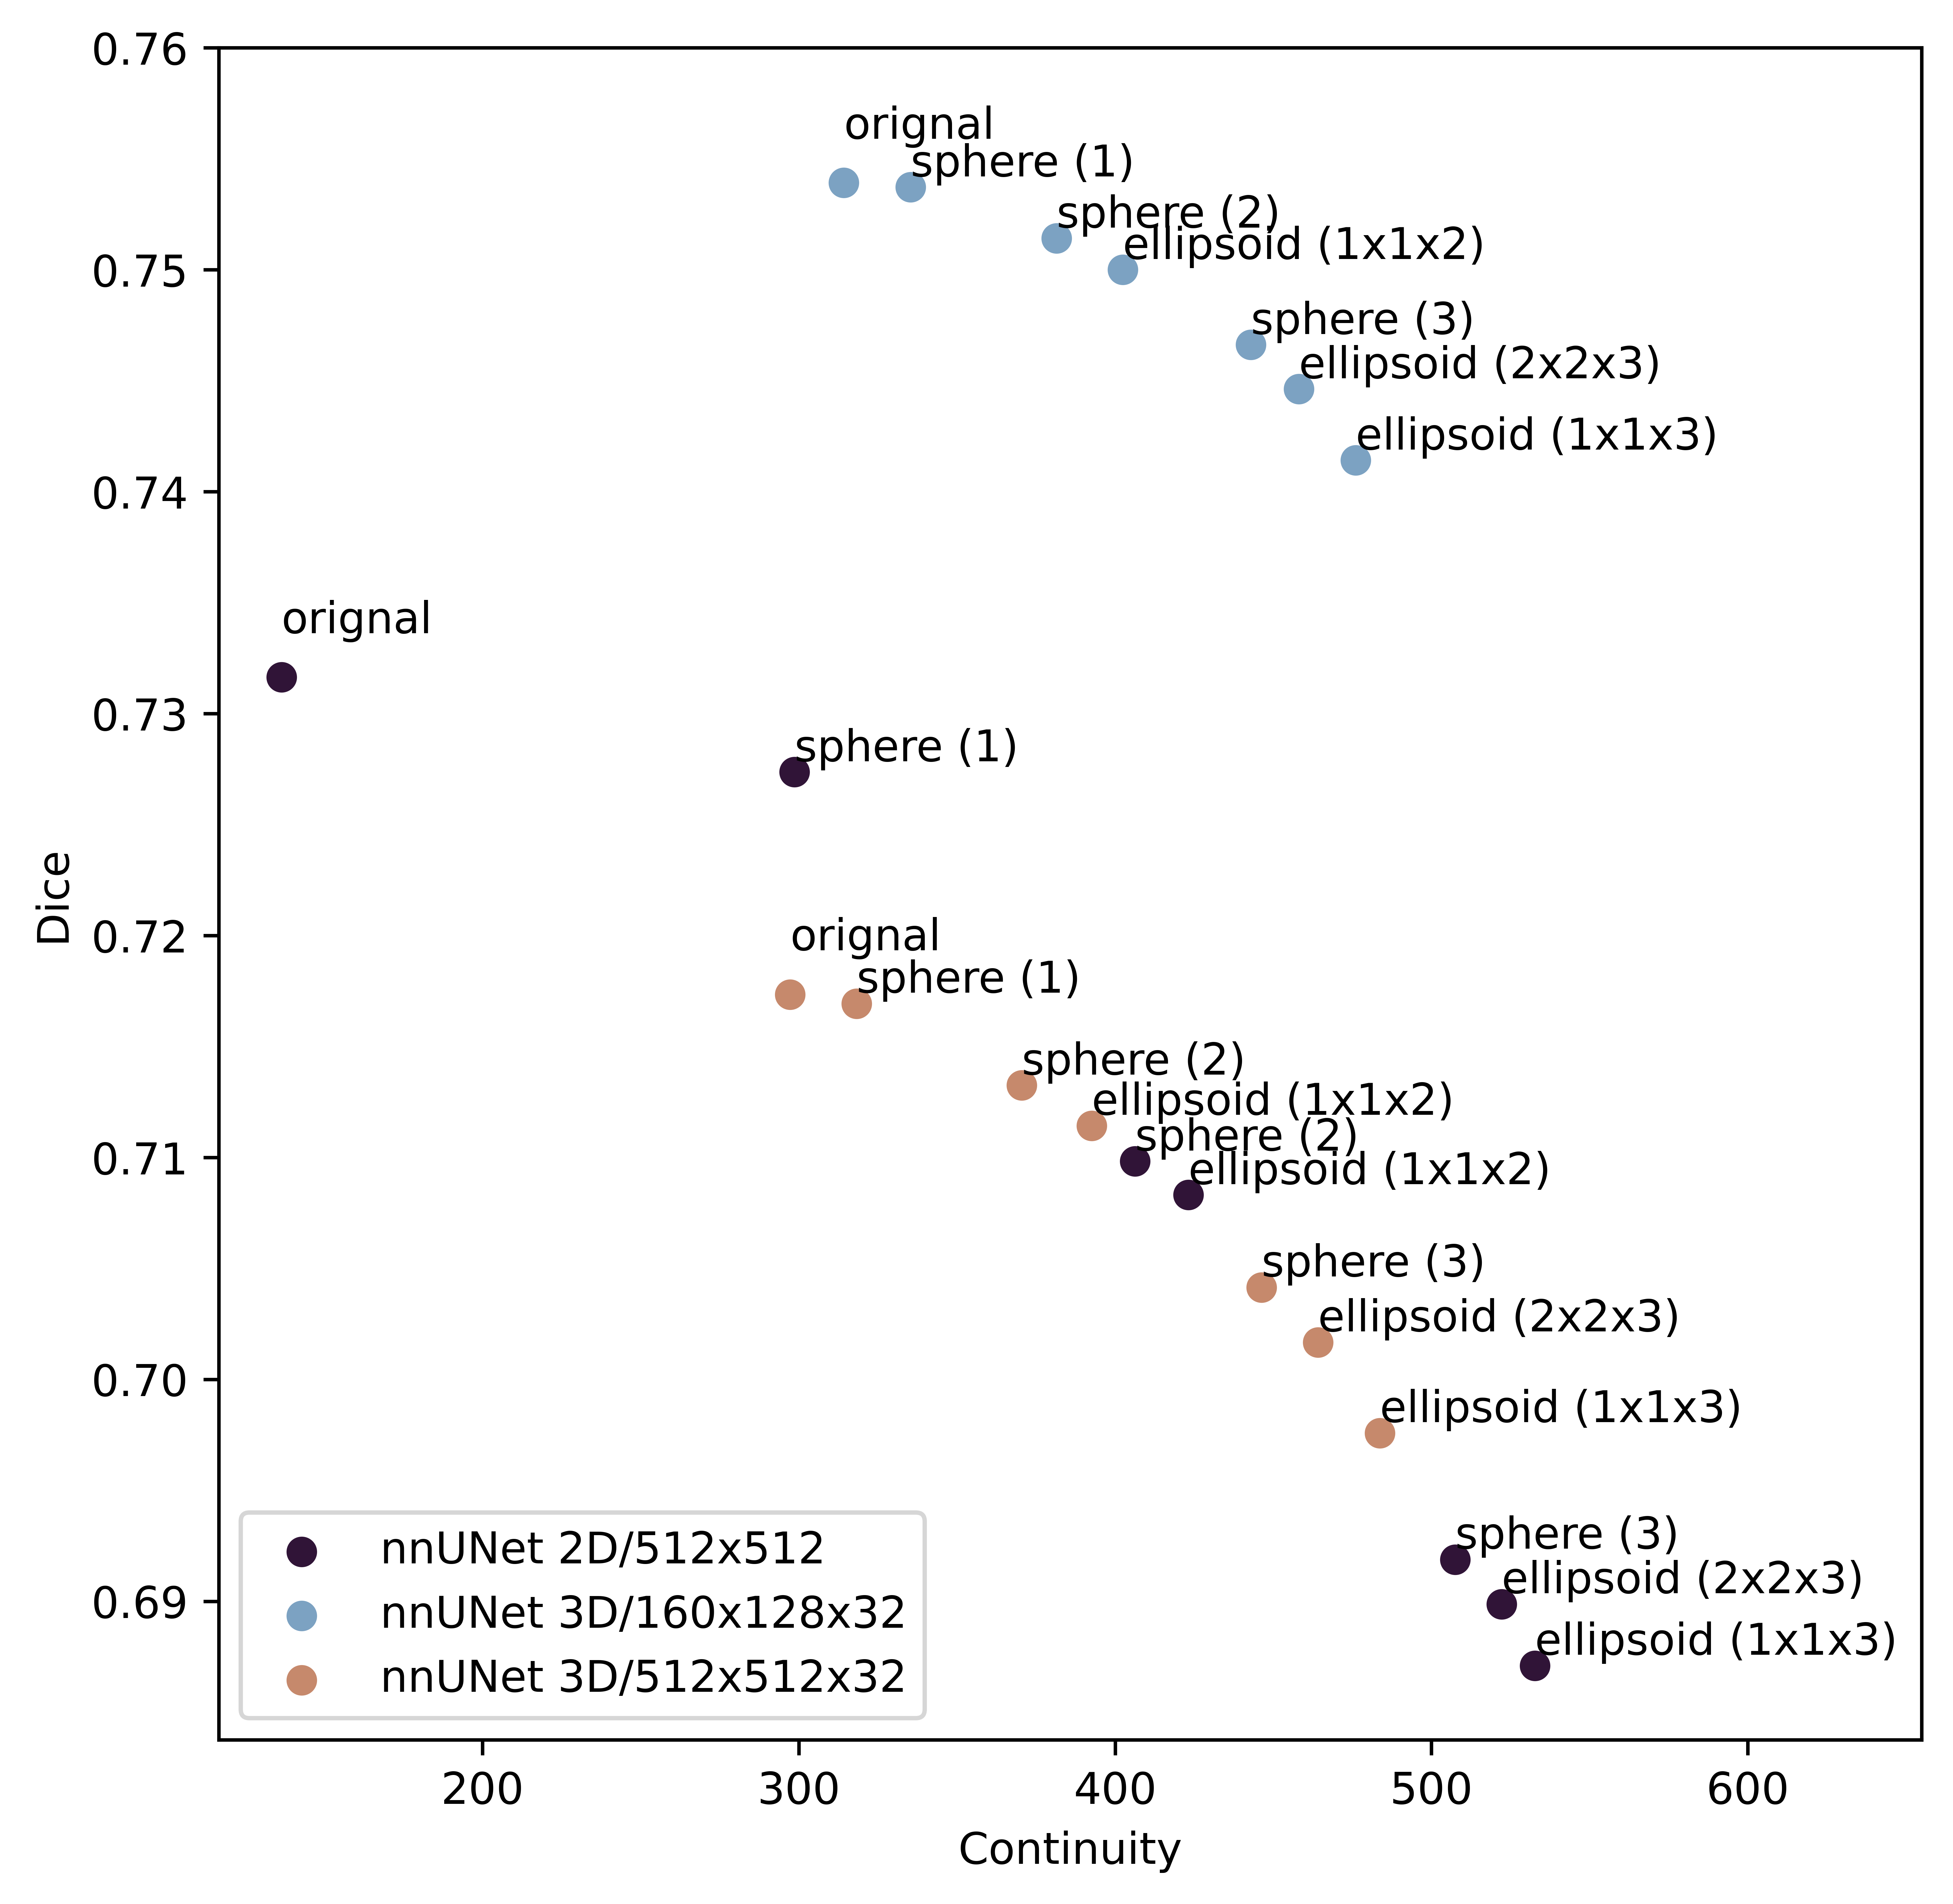
\includegraphics[width=0.5\linewidth]{figures/result_nnunet_dice_and_continuity.png}
    \caption{A plot showing the relationship between Dice scores and continuity as smoothing is increasingly applied. Original denotes the initial segmentation, while the others indicate the kernel shape and size used in smoothing. The size is denoted in $W\times H\times D$ notation.}
    \label{fig:nnunet-continuity-vs-correctness}
\end{figure}

As the kernel shape and size change, the segmentation becomes more continuous at the expense of a decrement in the Dice score. The trade-off varies across models, with the 3D nnUNet better retaining the performance while providing better continuity. 

\section{SuPreM}
We evaluated three configurations of the SwinUNTER model, as described in Section~\ref{sec:design:suprem}. Our findings indicate that SuPreM pre-training on SwinUNTER yields the best results with an average Dice score of $0.631\pm0.030$. This score is statistically higher than those of the other two configurations. SuPreM pre-training provides superior features for calcium segmentation compared to self-supervised learning and training from scratch. The results are summarized in Figure~\ref{fig:suprem-results}.

\begin{figure}[hbt]
    \centering
    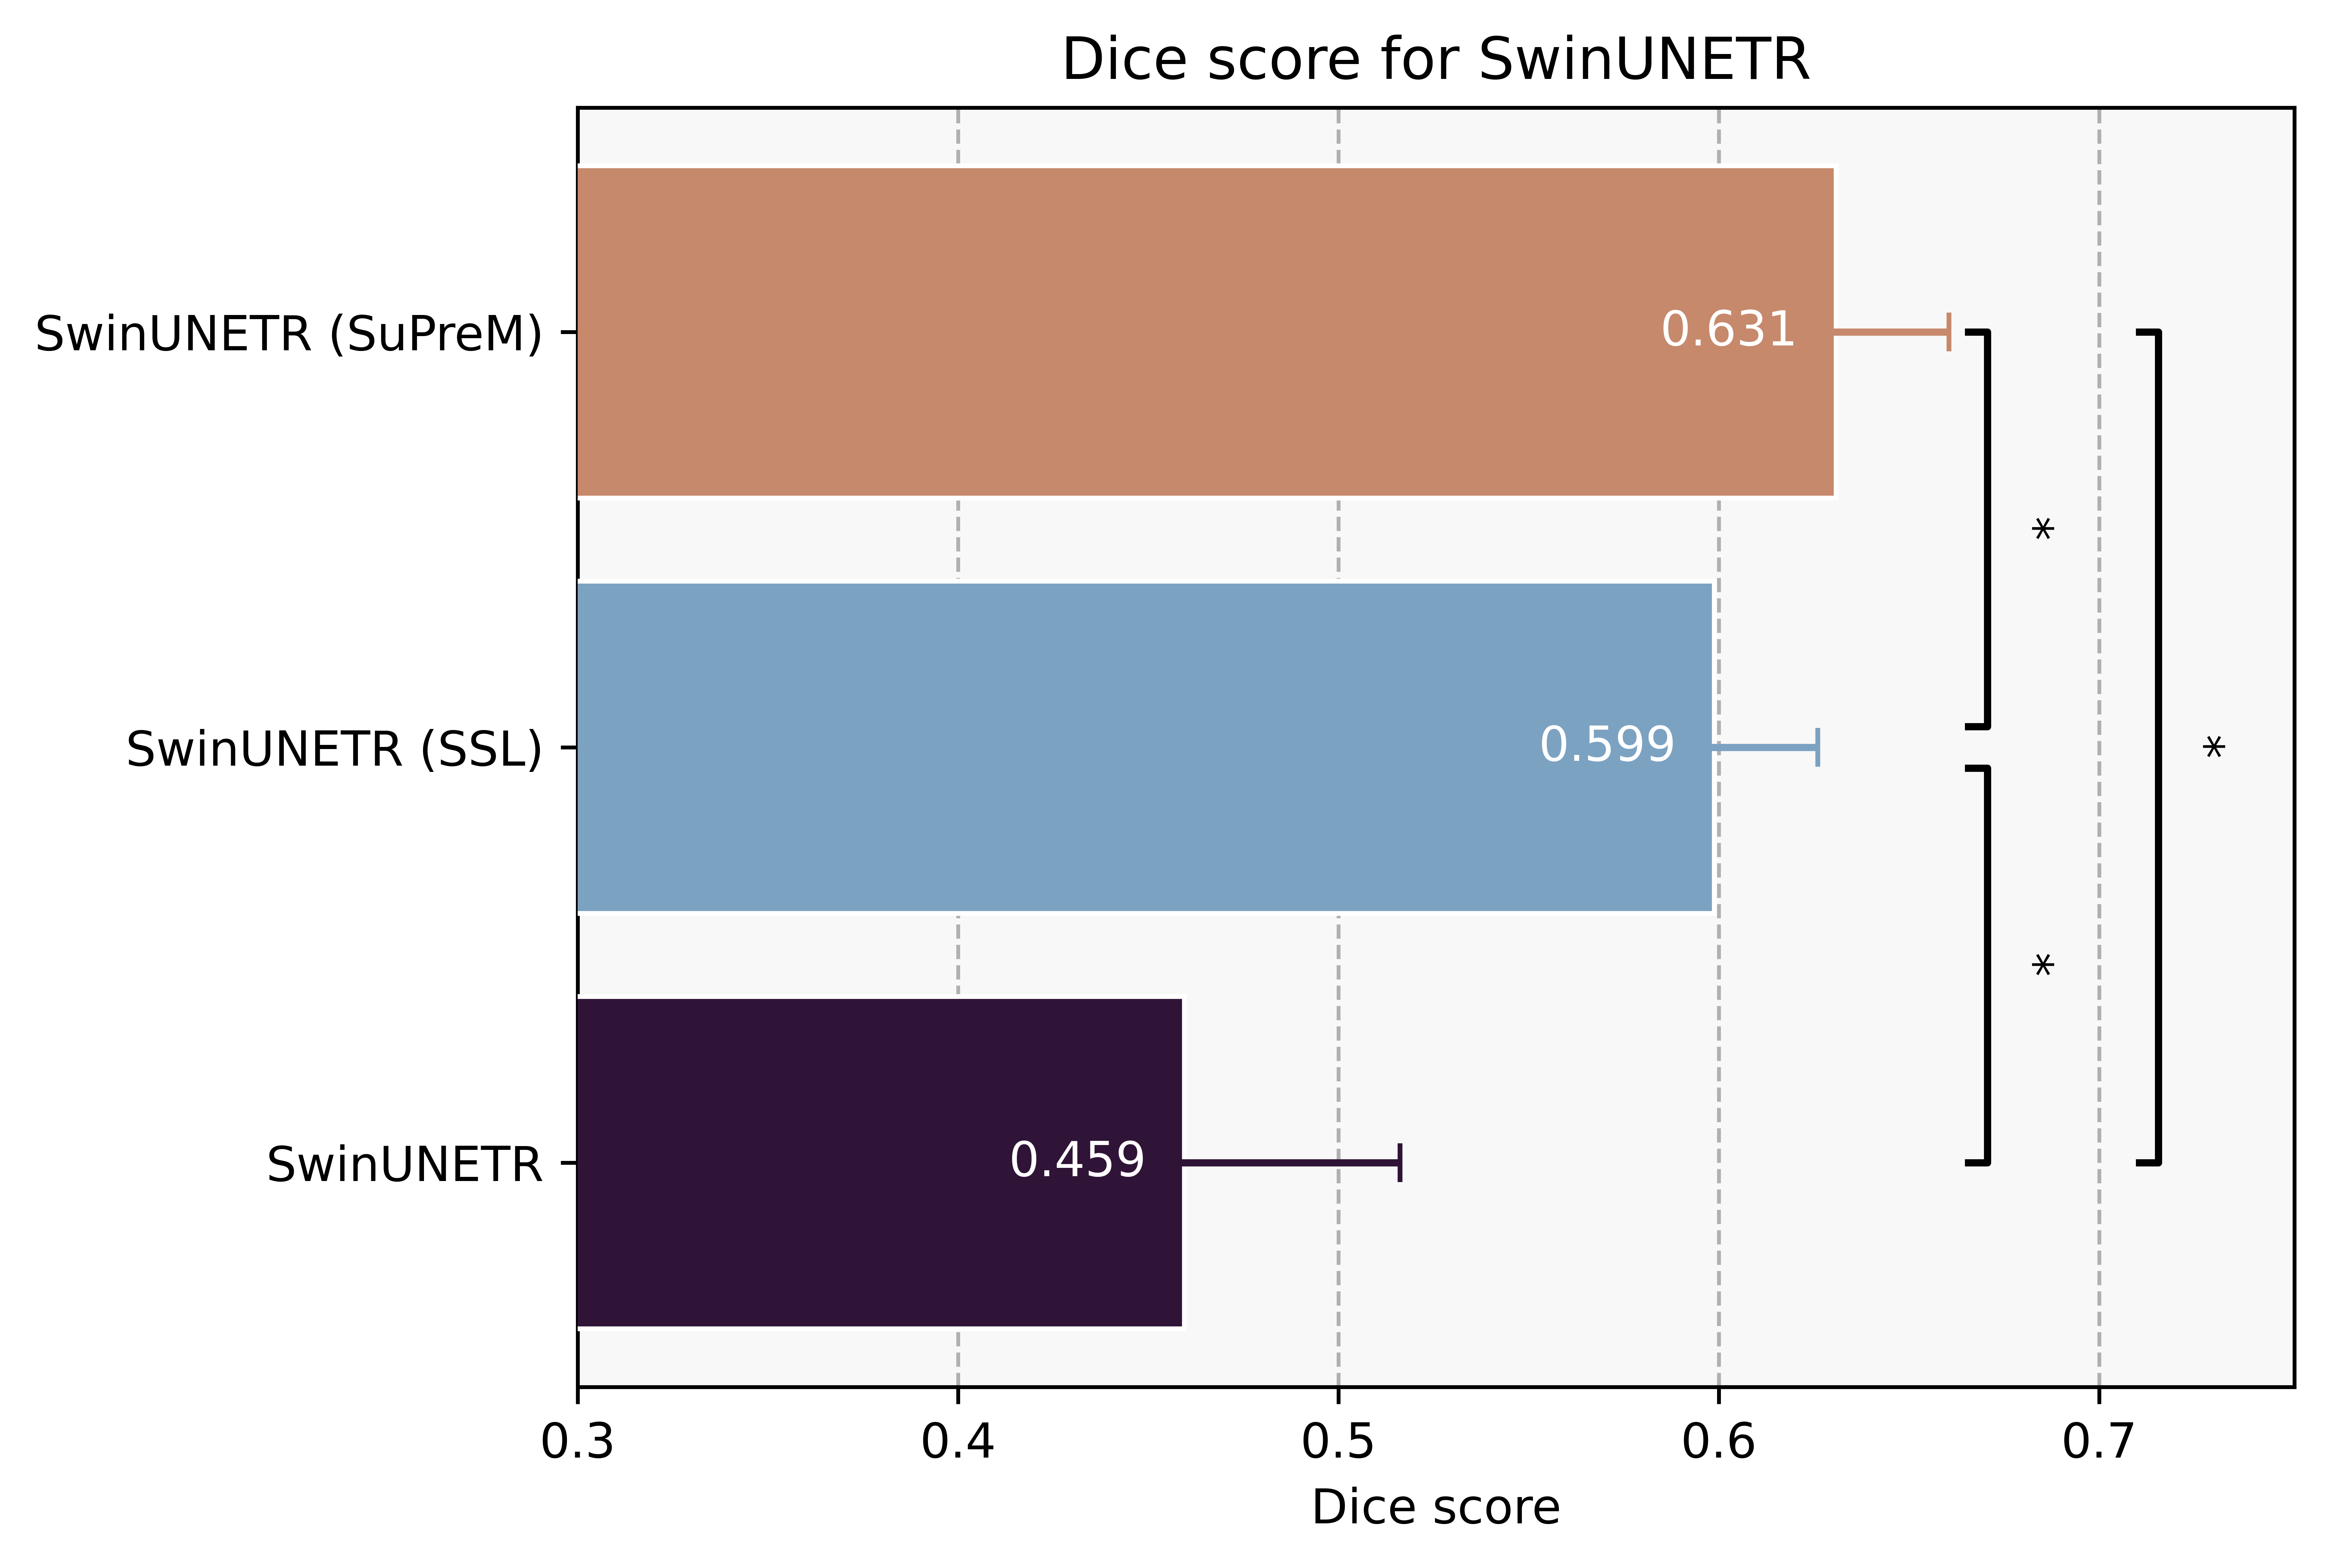
\includegraphics[width=0.5\linewidth]{figures/result_SwinUNETR_results.png}
    \caption{Dice score of SuPreM's SwinUNTER model. In the parenthesis indicate pre-training algorithms. SuPreM pre-training on SwinUNTER yields the best results and is significantly better than both self-supervised pre-training and training from scratch.}
    \label{fig:suprem-results}
\end{figure}

However, when comparing the result of the SuPreM pre-trained SwinUNTER model with that of the best 2D nnUNet model, the 2D nnUNet model outperforms the SuPreM model (see Figure~\ref{fig:transformer-results}). This will be discussed in the following section.

\section{Transformers-based Models}
We find that the best 3D nnUNet model outperforms all transformer-based models. This may be attributed to fundamental differences between CNN and transformer architectures. CNNs are designed to learn local features, while transformers are designed to learn global features. Calcium plaques in OCT images are localized, making CNNs more suitable for this task. This is also supported by the fact that, in CNNs, increasing the patch size in the width and height dimensions of the 3D nnUNet does not improve performance, while reducing the patch size in the depth dimension significantly improves performance (see Section~\ref{sec:result:nnunet}). The effectiveness of the SegFormer, ViT (RADIO), and SwinUNTER (SuPreM) compared to the nnUNet is summarized in Figure~\ref{fig:transformer-results}.

\begin{figure}[hbt]
    \centering
    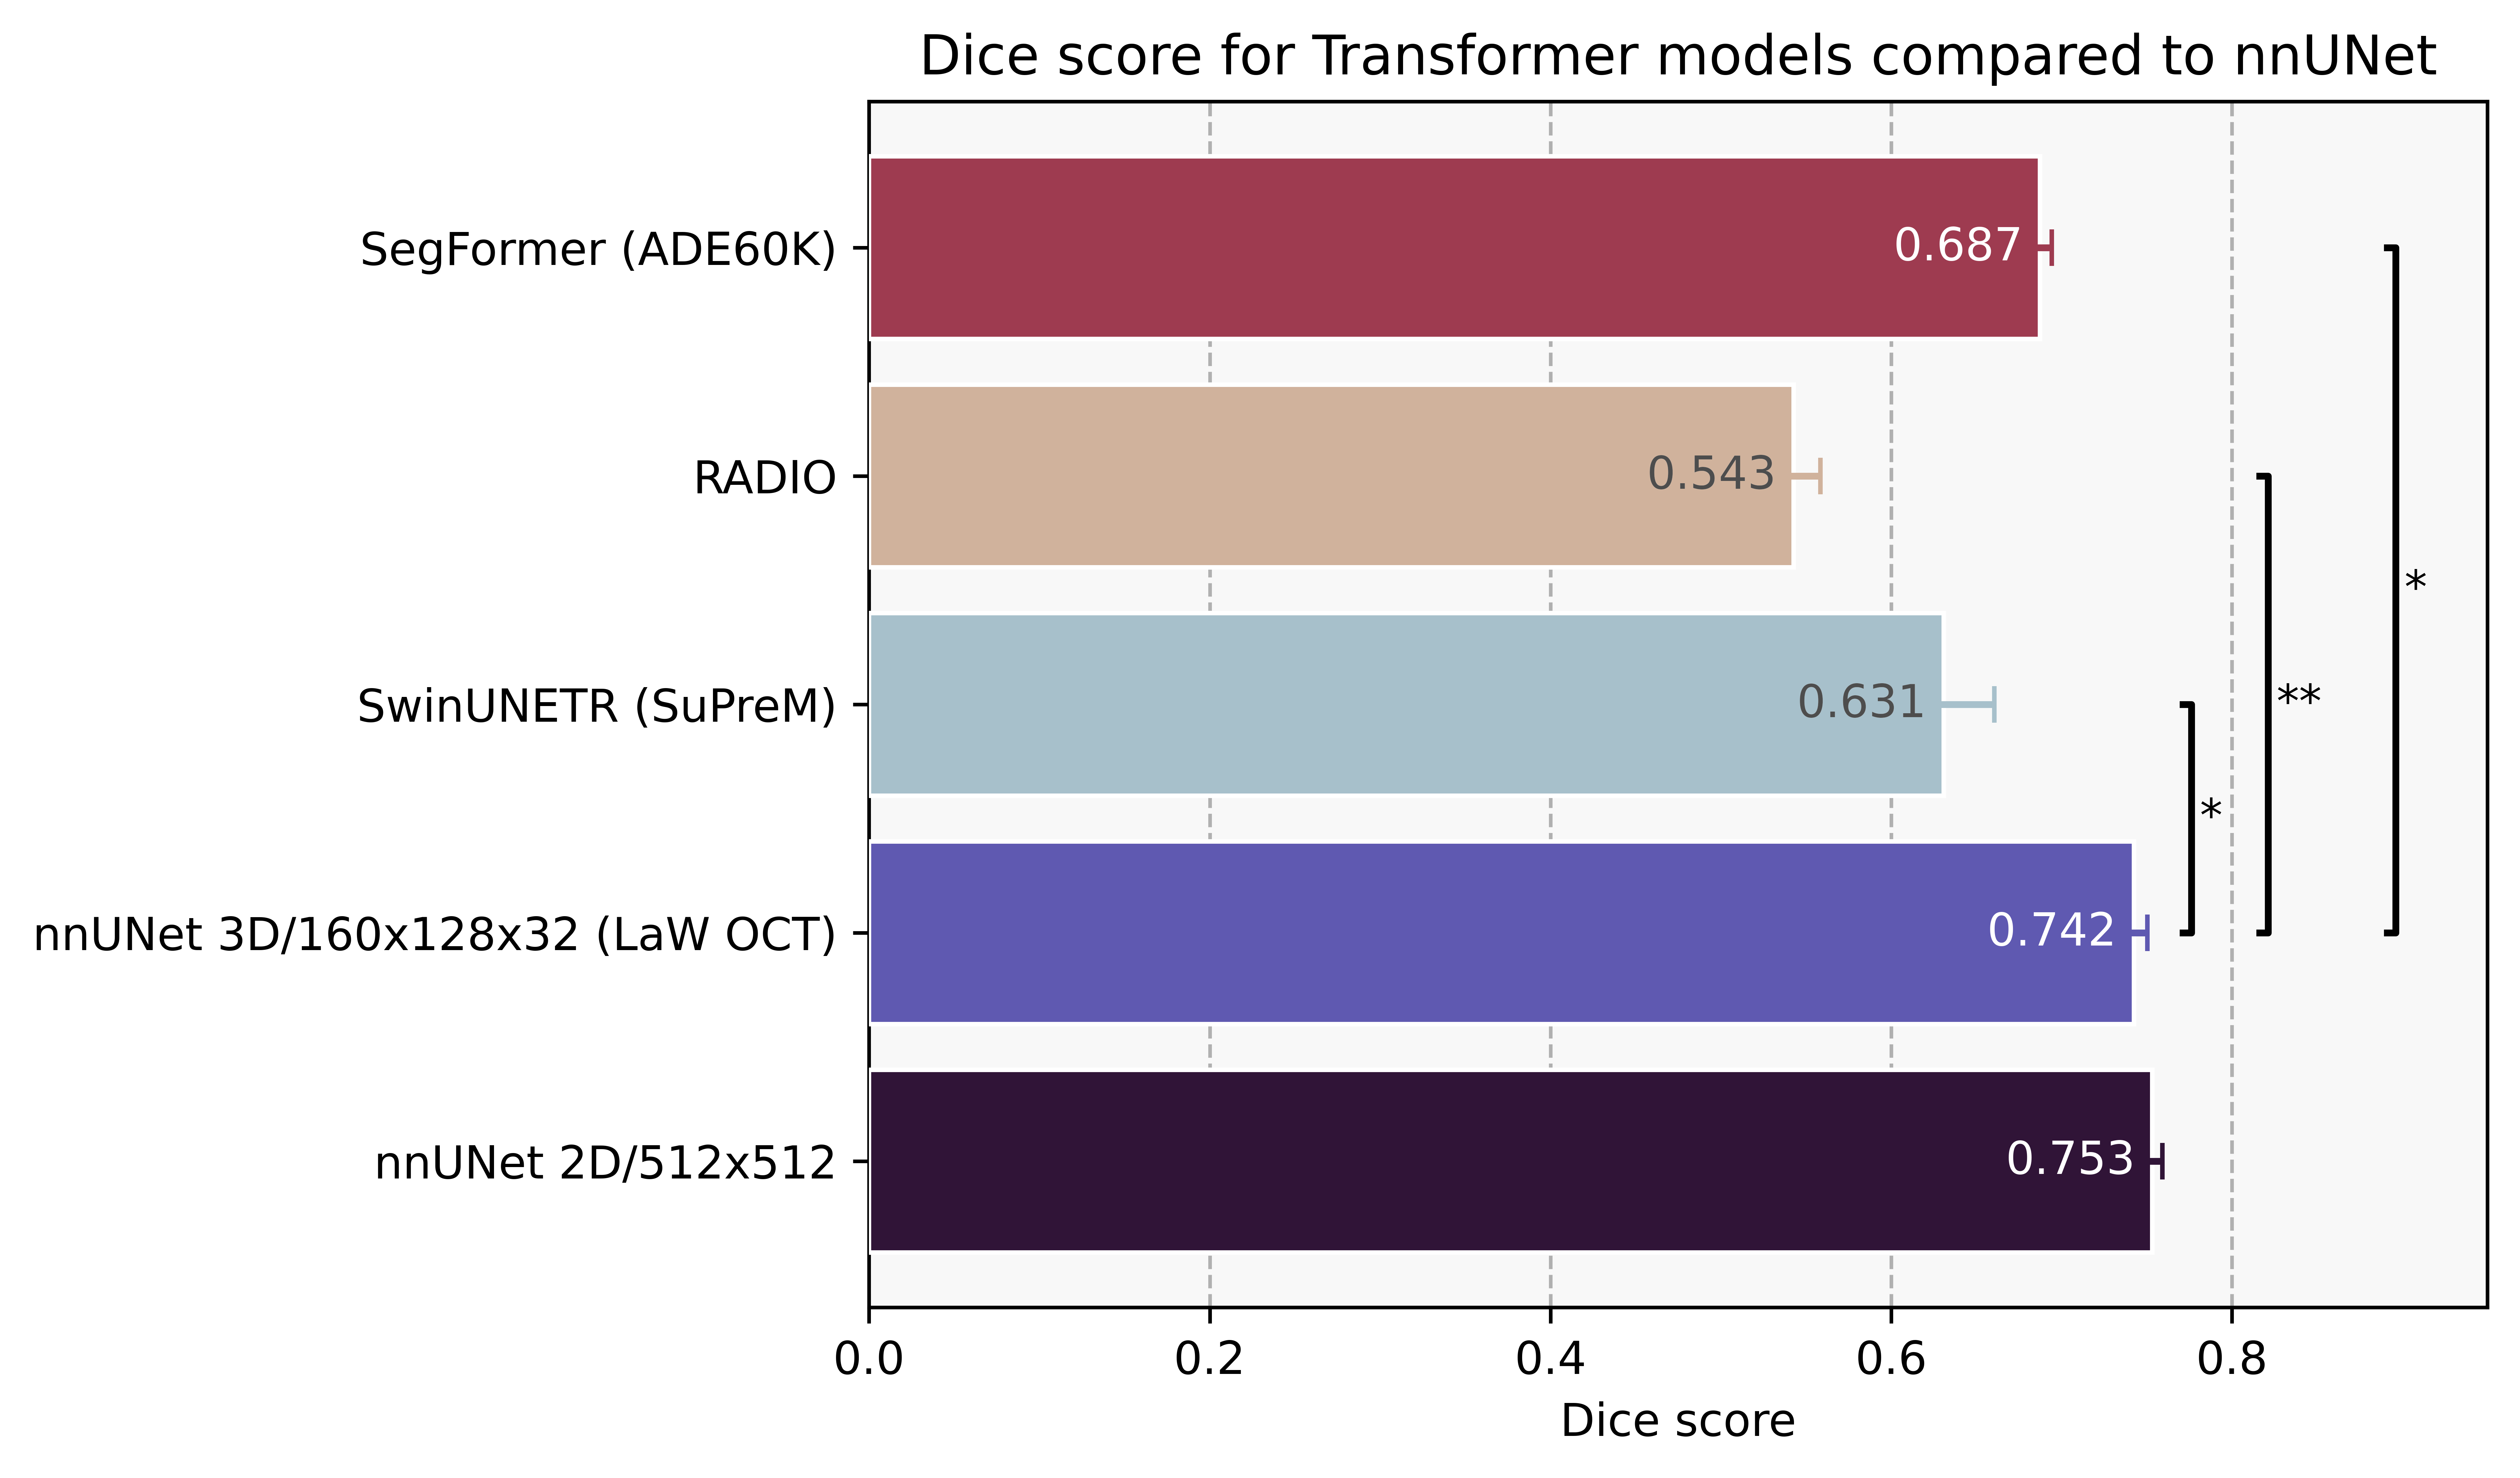
\includegraphics[width=0.6\linewidth]{figures/result_nnUNet_vs_Transformer_results.png}
    \caption{Dice scores of transformer-based models compared to those of the nnUNet. Compared to the best 3D nnUNet model pre-trained on the LaW OCT dataset, Dice scores of transformer-based models are statistically significantly lower.}
    \label{fig:transformer-results}
\end{figure}

\section{V-JEPA}
Each experiment is denoted by its architecture and its decoder head. The dataset V-JEPA was pre-trained on is indicated in the parenthesis. The control experiment, \textbf{ViT + Attentive*}, is the ViT model followed by an attentive decoder head, with intensive data augmentation and positive data sampling, but without V-JEPA pre-training. The results of different decoder heads are summarized in Figure~\ref{fig:vjepa-decoder-results}.

There is no significant difference between the various decoder heads. However, the representation learned by V-JEPA on VideoMix2M, namely \textbf{ViT + Attentive* (V-JEPA VideoMix2M)}, significantly improves the performance of the ViT model on calcium segmentation (\textbf{ViT + Attentive*}). This highlights the usefulness of V-JEPA pre-training.

\begin{figure}[hbt]
    \centering
    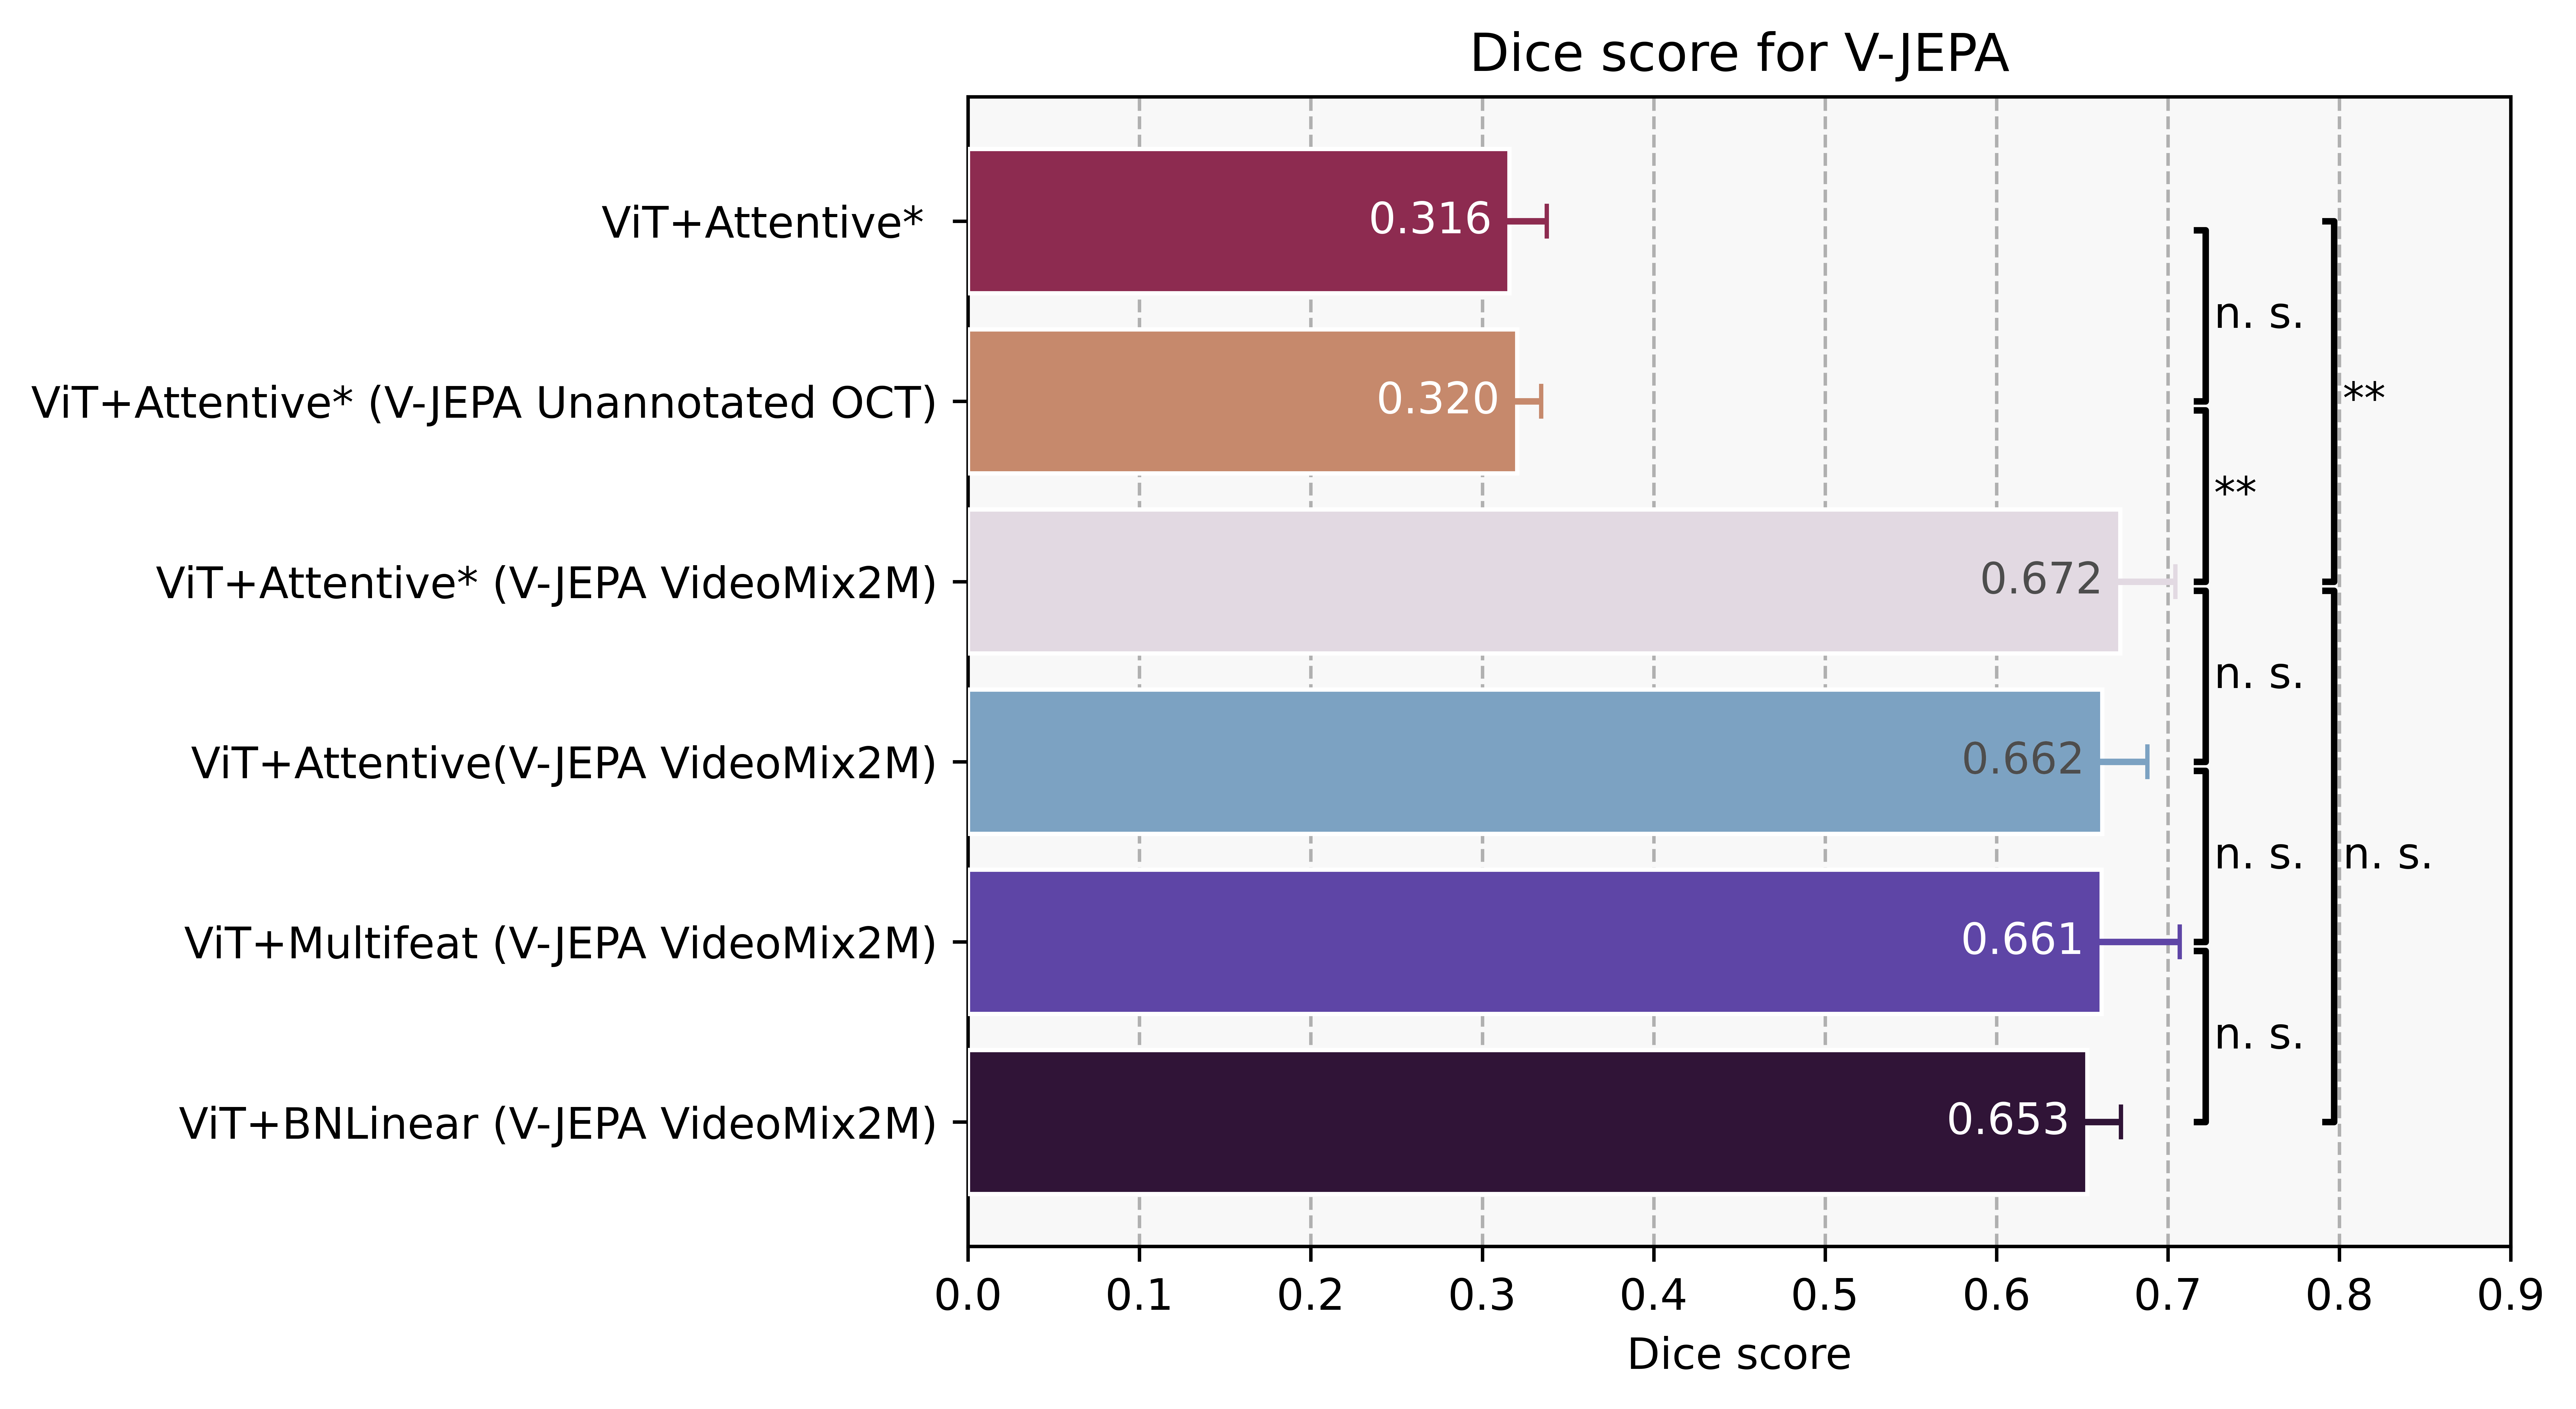
\includegraphics[width=0.75\linewidth]{figures/result_VJEPA_results.png}
    \caption{Dice score of V-JEPA's decoder head. BNLinear denotes batch normalization followed by linear projection. Attentive signifies the attentive decoder head. Attentive* indicates an attentive decoder head with more intensive data augmentation and positive data sampling. MultiFeat denotes the multi-features decoder head. The dataset V-JEPA was pre-trained on is indicated in the parenthesis.}
    \label{fig:vjepa-decoder-results}
\end{figure}

In addition to V-JEPA pre-trained on VideoMix2M, we also evaluated V-JEPA pre-trained on our unannotated OCT images, \textbf{ViT + Attentive* (V-JEPA Unannotated OCT)}. Pre-training on the unannotated OCT images did not improve the performance of the ViT model on calcium segmentation. This may be due to the size of the dataset. The unannotated OCT dataset consists of only 500 volumes, whereas VideoMix2M contains 2M videos. This demonstrates the importance of dataset scale for self-supervised learning on transformer-based models.

\section{CLIP}
We find that CLIP pre-training on co-registered OCT images significantly improves the performance of the 3D nnUNet model. In addition, CLIP is statistically comparable to the 3D nnUNet model pre-trained on the LaW OCT dataset. This shows that CLIP is as effective as supervised pre-training on the LaW OCT dataset, while the cost for co-registration is lower than the cost for annotating lumen and wall. The performance of CLIP pre-training on co-registered multi-modal OCT images is summarized in Figure~\ref{fig:clip-results}.

\begin{figure}[h]
    \centering
    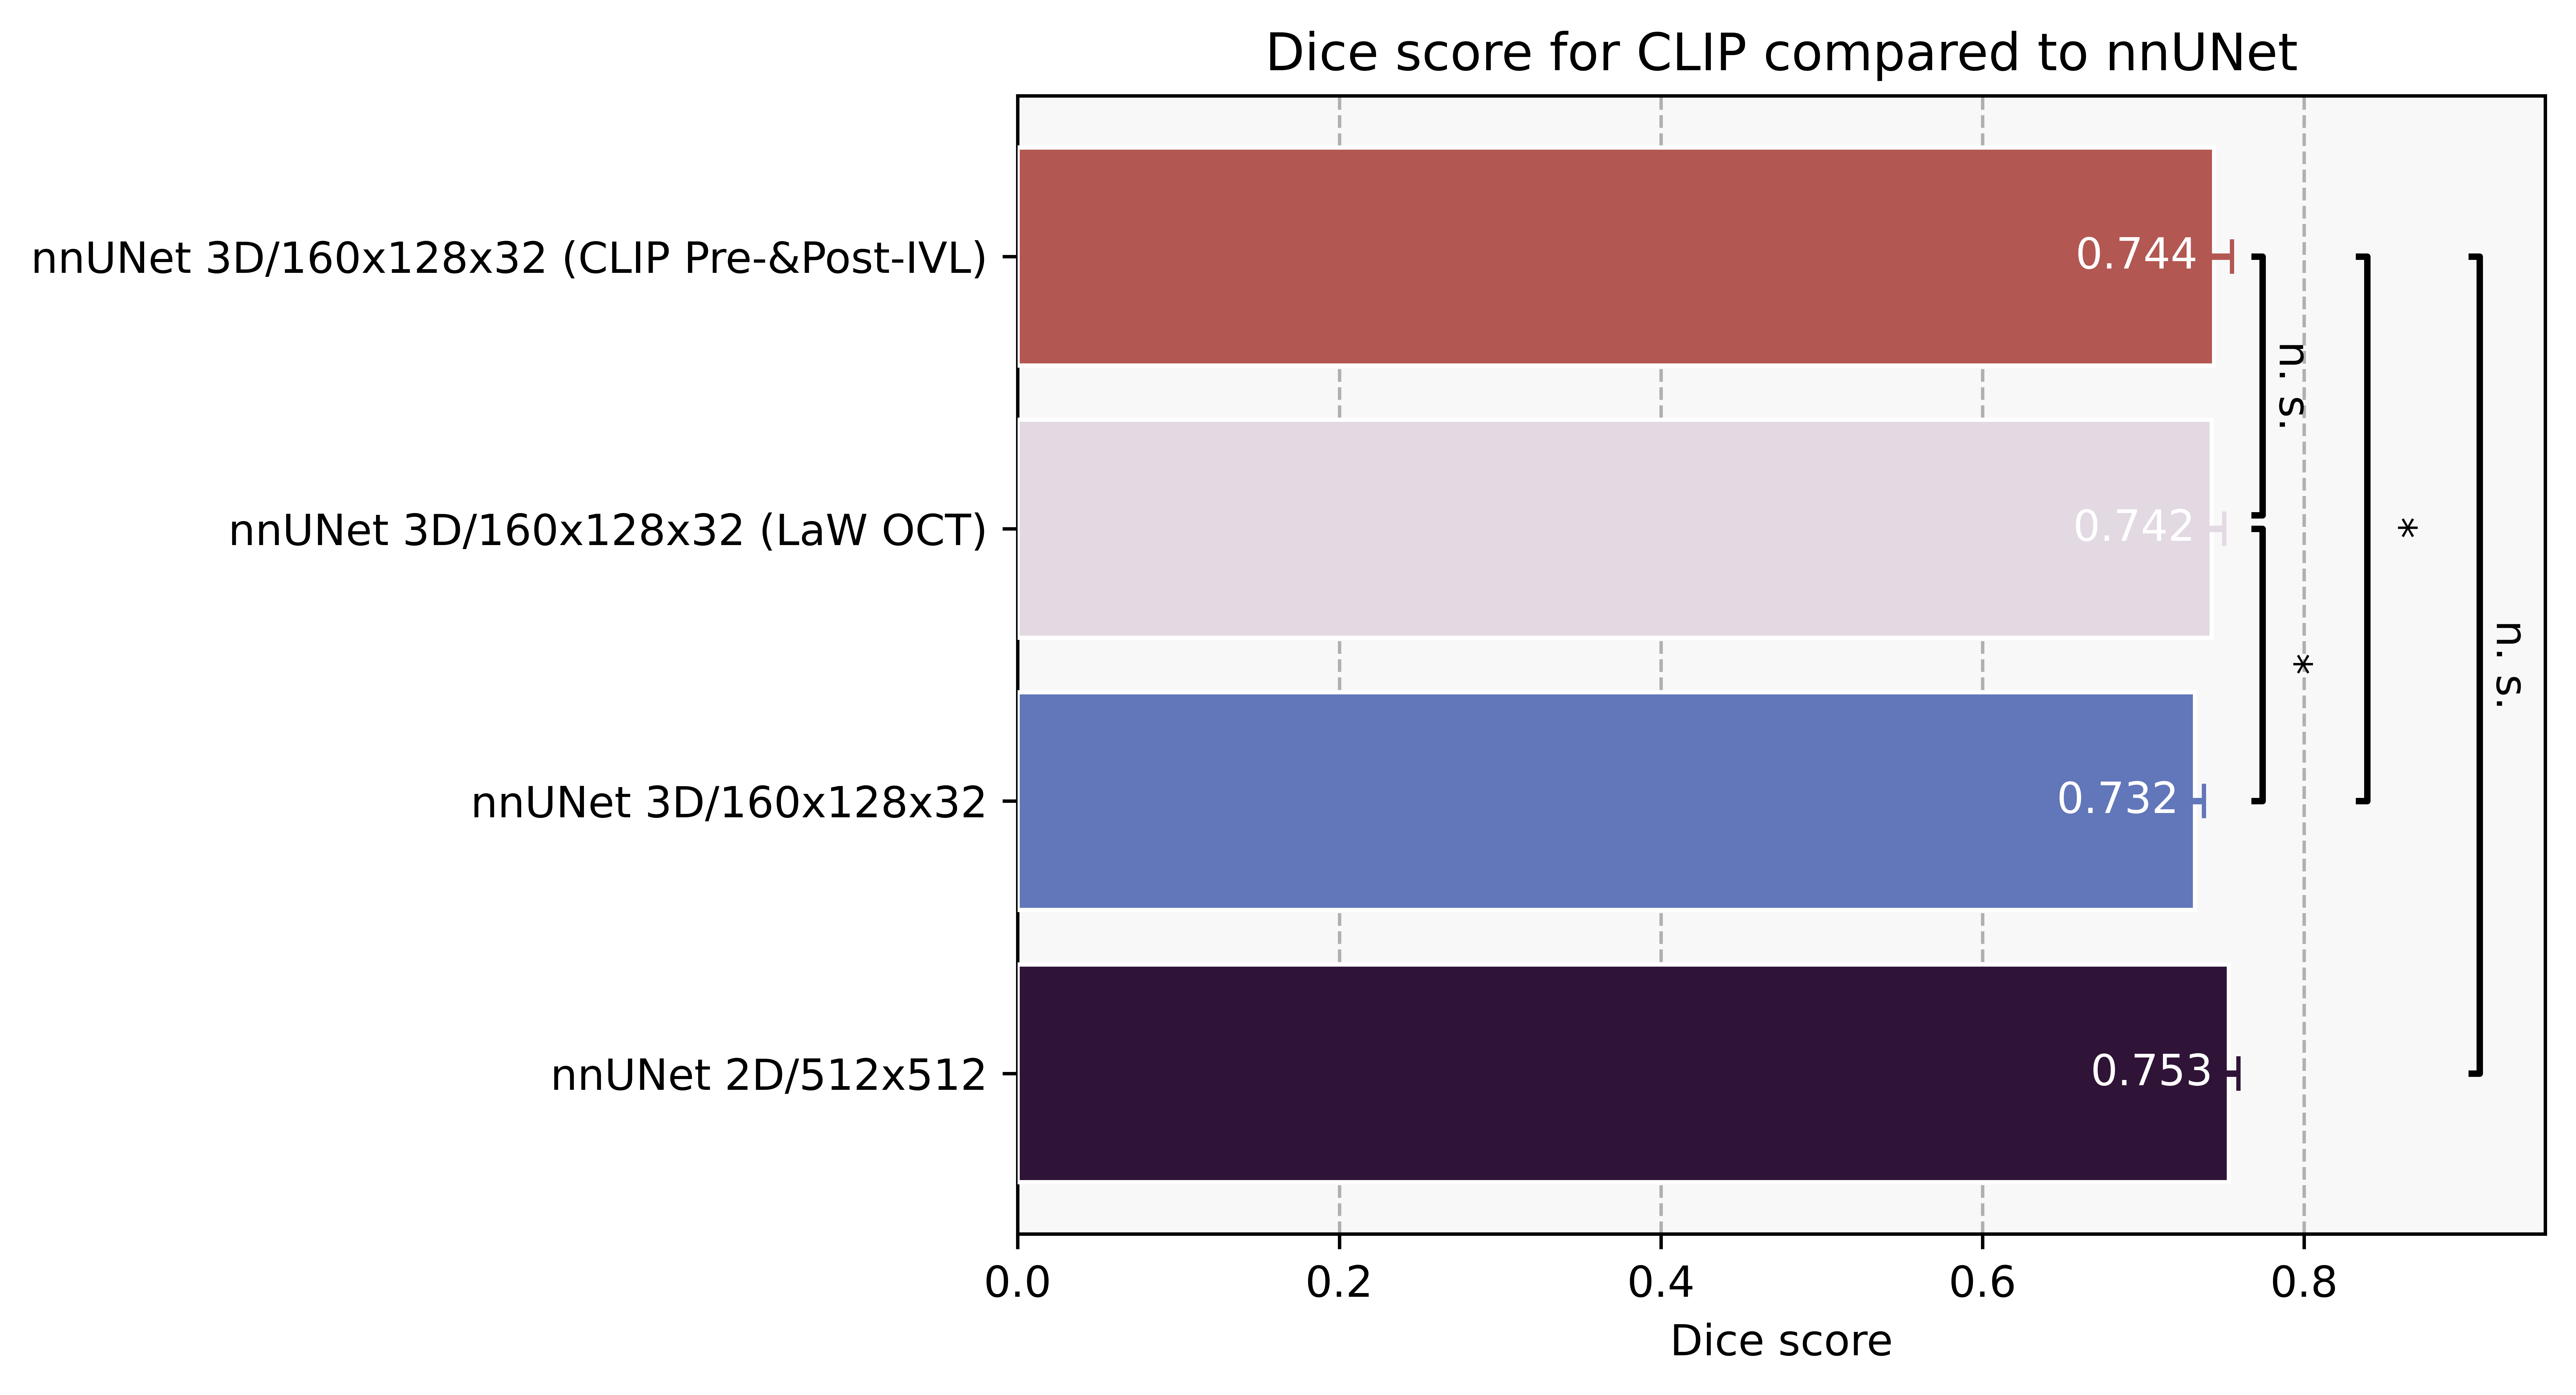
\includegraphics[width=0.65\linewidth]{figures/result_nnUNet_and_CLIP_results.png}
    \caption{Dice score of CLIP on Calcium OCT dataset compared to nnUNet. The algorithms used for pre-training are indicated in the parenthesis. The LaW OCT is the supervised pre-training on the Lumen and Wall OCT dataset. CLIP is the pre-training on co-registered multi-modal OCT images.
    }
    \label{fig:clip-results}
\end{figure}

The success of CLIP pre-training may result from the fact that aligning Pre-IVL and Post-IVL requires the model to learn the features of the lumen and wall, which has been proven to be useful for calcium segmentation in nnUNet (LaW OCT). To prove this, we visualize the PCA of the features learned by CLIP compared to the features output from the initial weight of the model. 

\begin{figure}[h]
    \centering
    \begin{subfigure}[t]{0.5\textwidth}
        \centering
        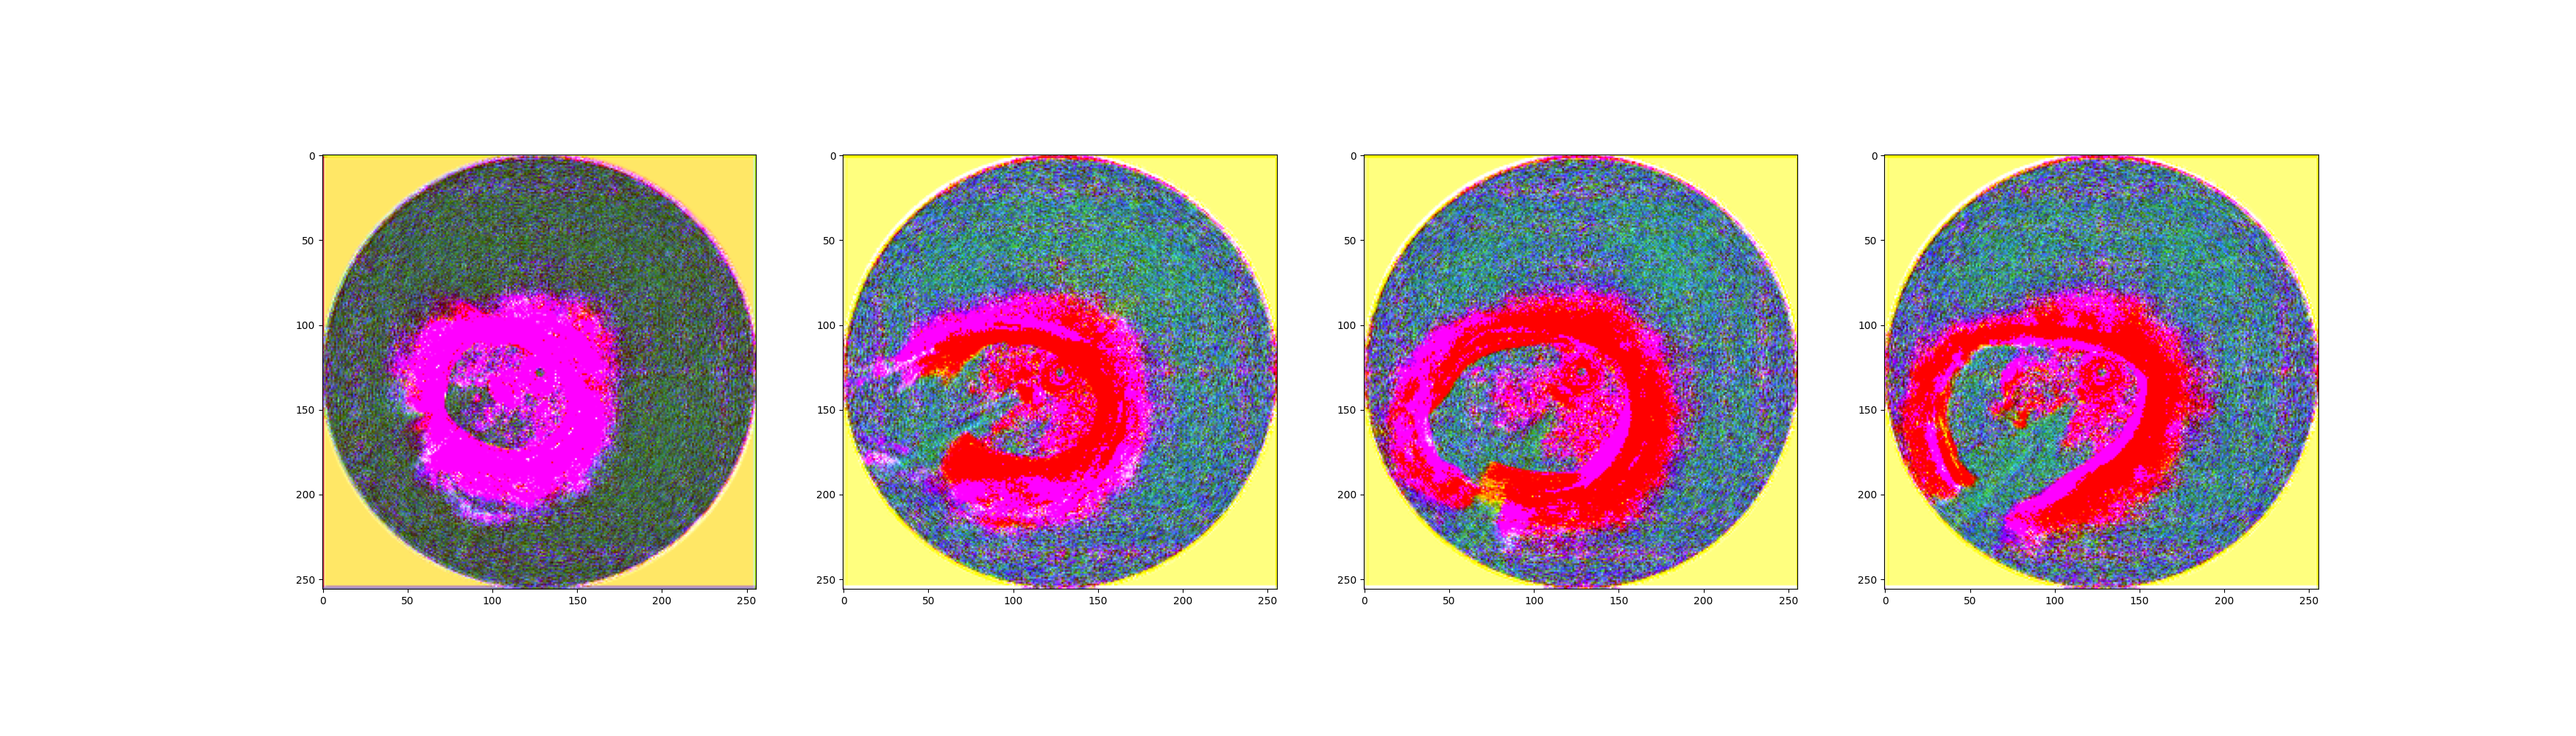
\includegraphics[width=\linewidth]{figures/discussion_default_feature_map_batch0_feature1.png}
        \caption{PCA of the output of the features from the initial weight of the model.}
        \label{fig:pca-initial}
    \end{subfigure}%
    \begin{subfigure}[t]{0.5\textwidth}
        \centering
        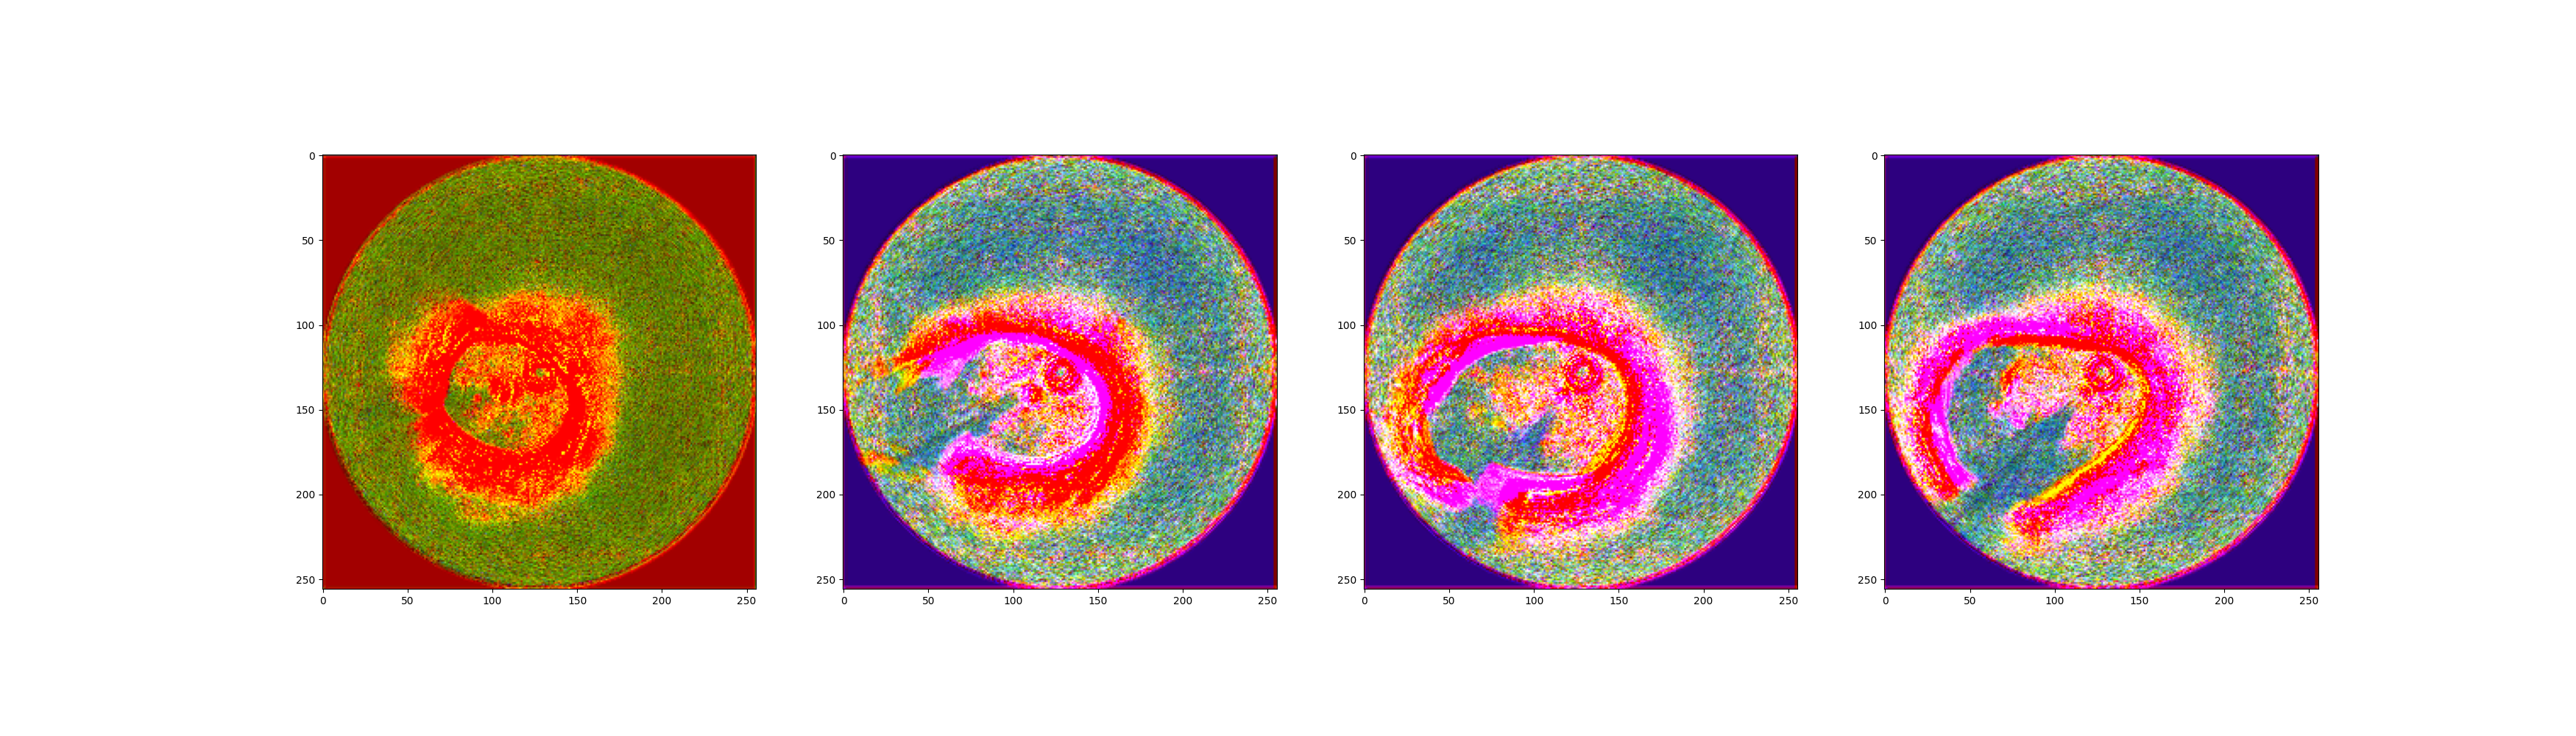
\includegraphics[width=\linewidth]{figures/discussion_clip_feature_map_batch0_feature1.png}
        \caption{PCA of the features learned by CLIP.}
        \label{fig:pca-clip}
        
    \end{subfigure}
    \caption{PCA of the output of the features from the initial weight of the model and the features learned by CLIP. CLIP pre-training gives more distinguishable features on the walls than those from the initial weight of the model. 
    % This can be the reason why CLIP pre-training improves the performance of the model.
    }
\end{figure}

The dataset used in CLIP is co-registered Pre-IVL and Post-IVL. Therefore, the author suggests similar experiments be further studied on the co-registered Pre-IVL and Post-Stent dataset.

\section{Genesis}
Pre-training Genesis on unannotated OCT images results in a Dice score of $0.744\pm0.000$ on the Calcium OCT dataset. Furthermore, Genesis significantly improves the performance of the 3D nnUNet model and performs comparably to the best 2D nnUNet and the pre-trained 3D nnUNet on the LaW OCT dataset, while not requiring additional data annotations. The results and statistical tests are summarized in Figure~\ref{fig:genesis-results}.

\begin{figure}[h]
    \centering
    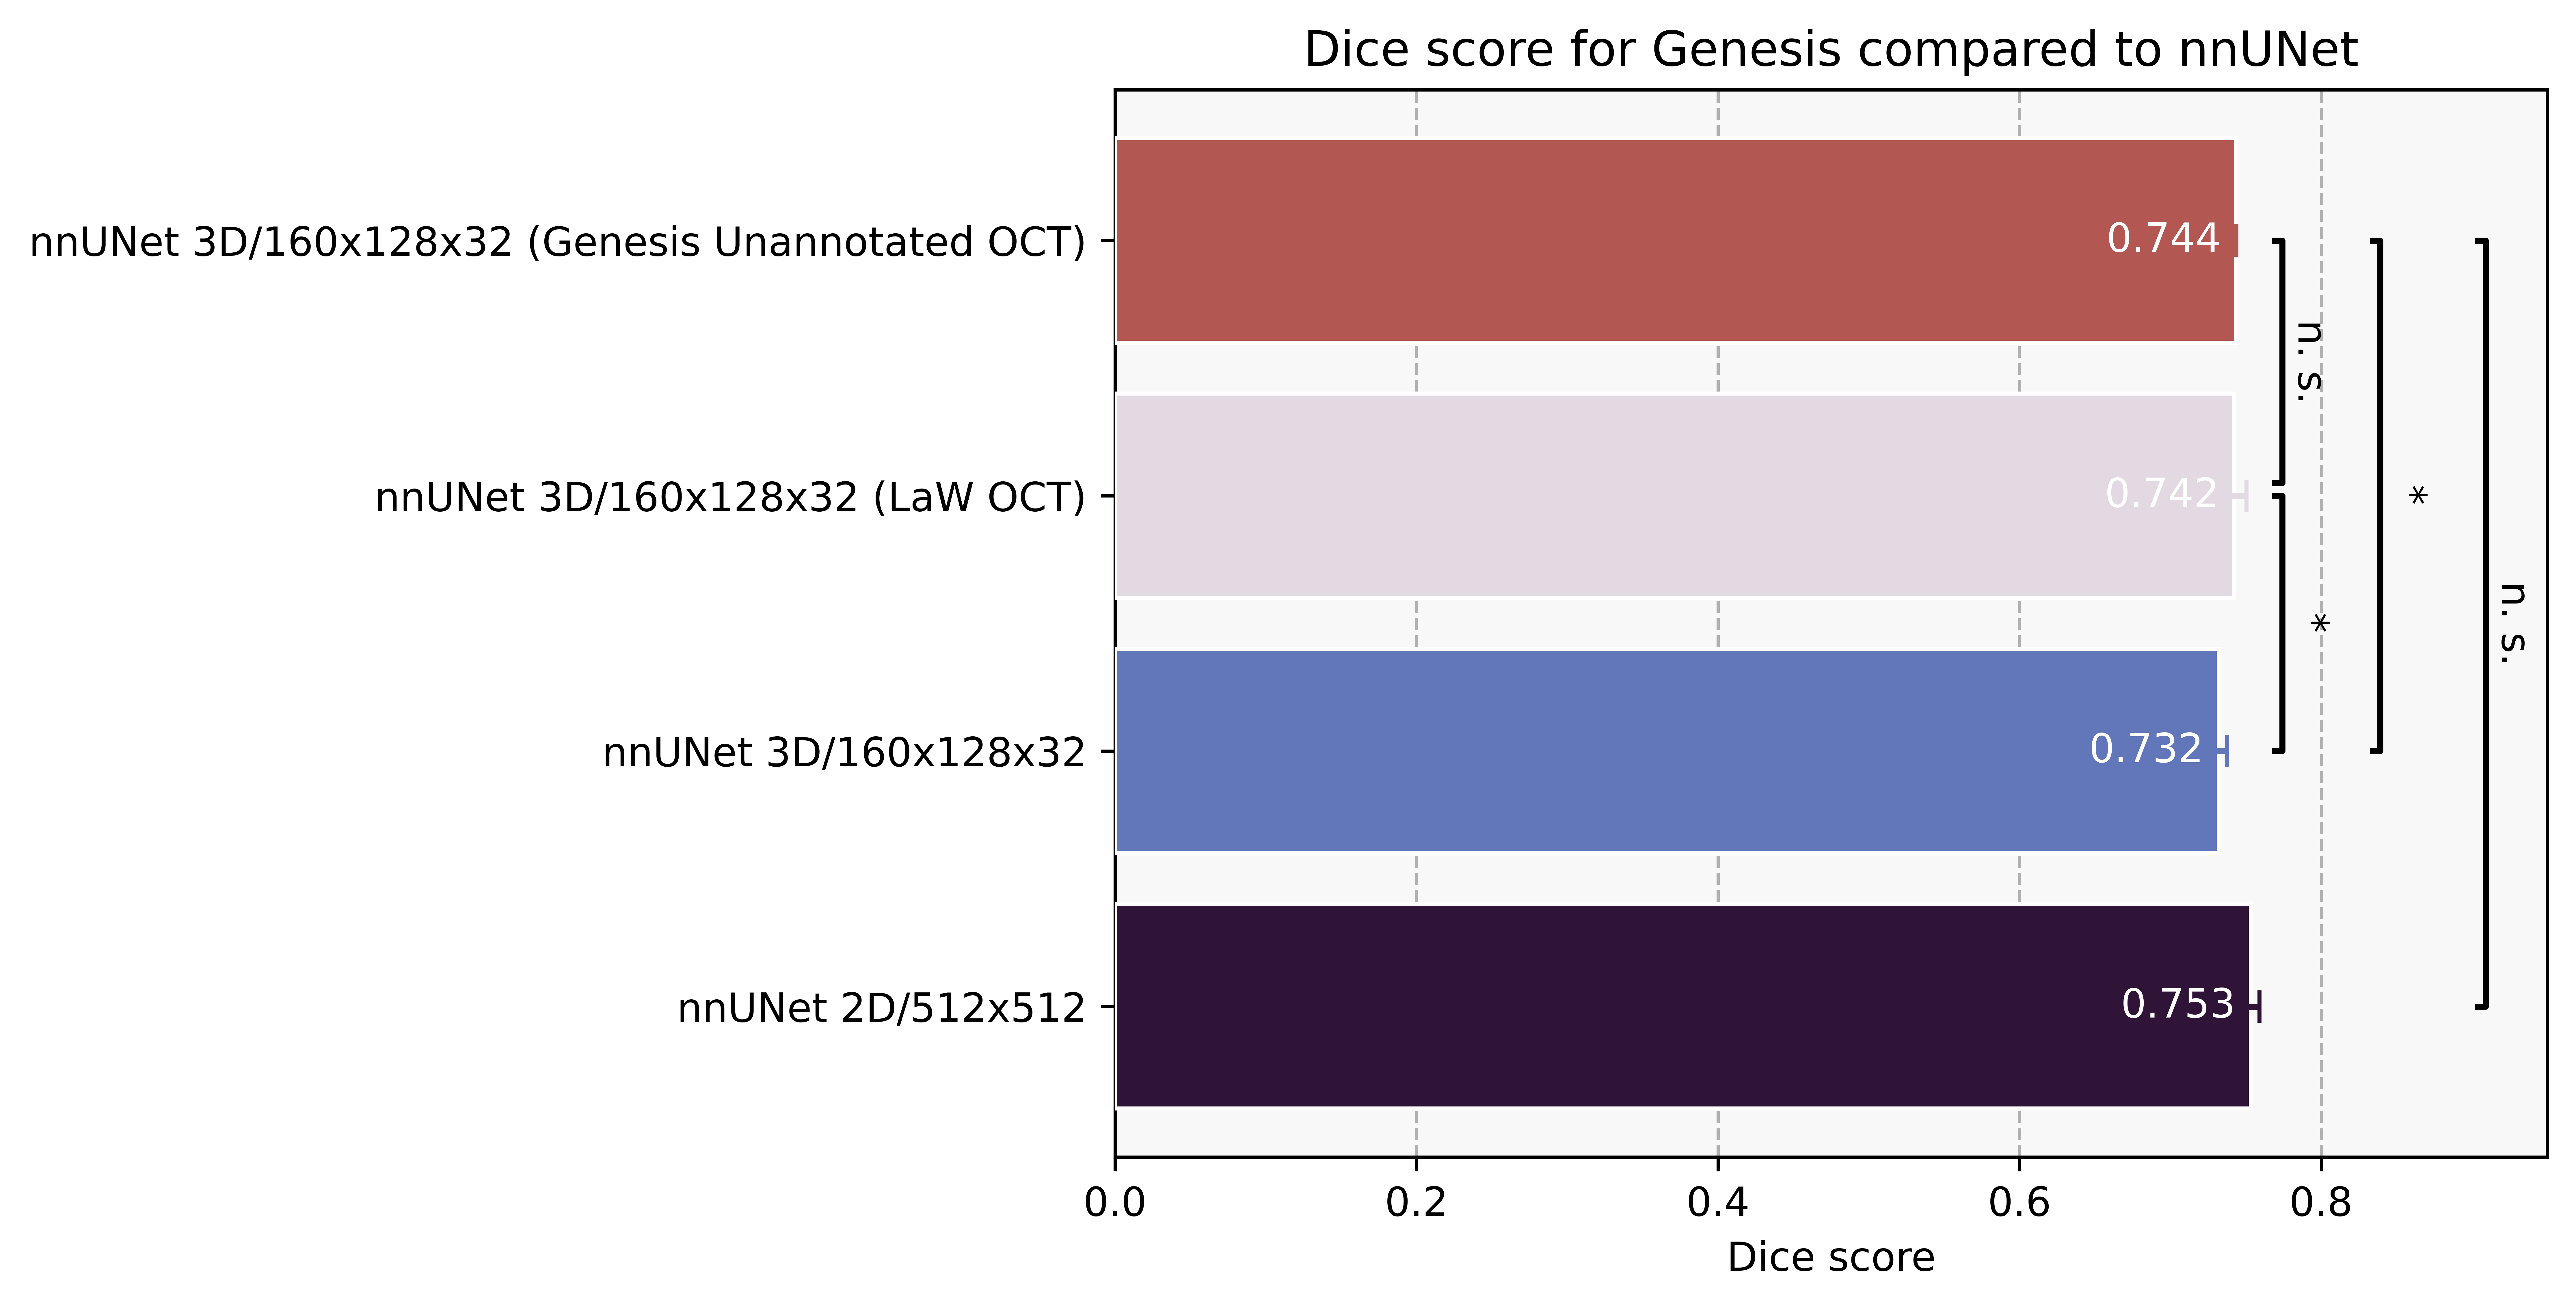
\includegraphics[width=0.65\linewidth]{figures/result_nnUNet_and_Genesis_results.png}
    \caption{a Dice score of Genesis on the Calcium OCT dataset compared to those of nnUNets. The dataset used for pre-training is indicated in the parenthesis.
    }
    \label{fig:genesis-results}    
\end{figure}


\section{Final Results}
The models are grouped into three categories: SSL for self-supervised learning models, Transformer for transformer-based models, and nnUNet for 2D and 3D CNN-based nnUNet models. V-JEPA on unannotated OCT is categorized under SSL, whereas V-JEPA on VideoMix2M is under Transformer, as it was only fine-tuned to the Calcium OCT dataset. Each result is statistically compared to the 2D nnUNet model, which has the highest average Dice score in our study. The results of the best models in each category are summarized in Figure~\ref{fig:results}.

\begin{figure}[hbt]
    \centering
    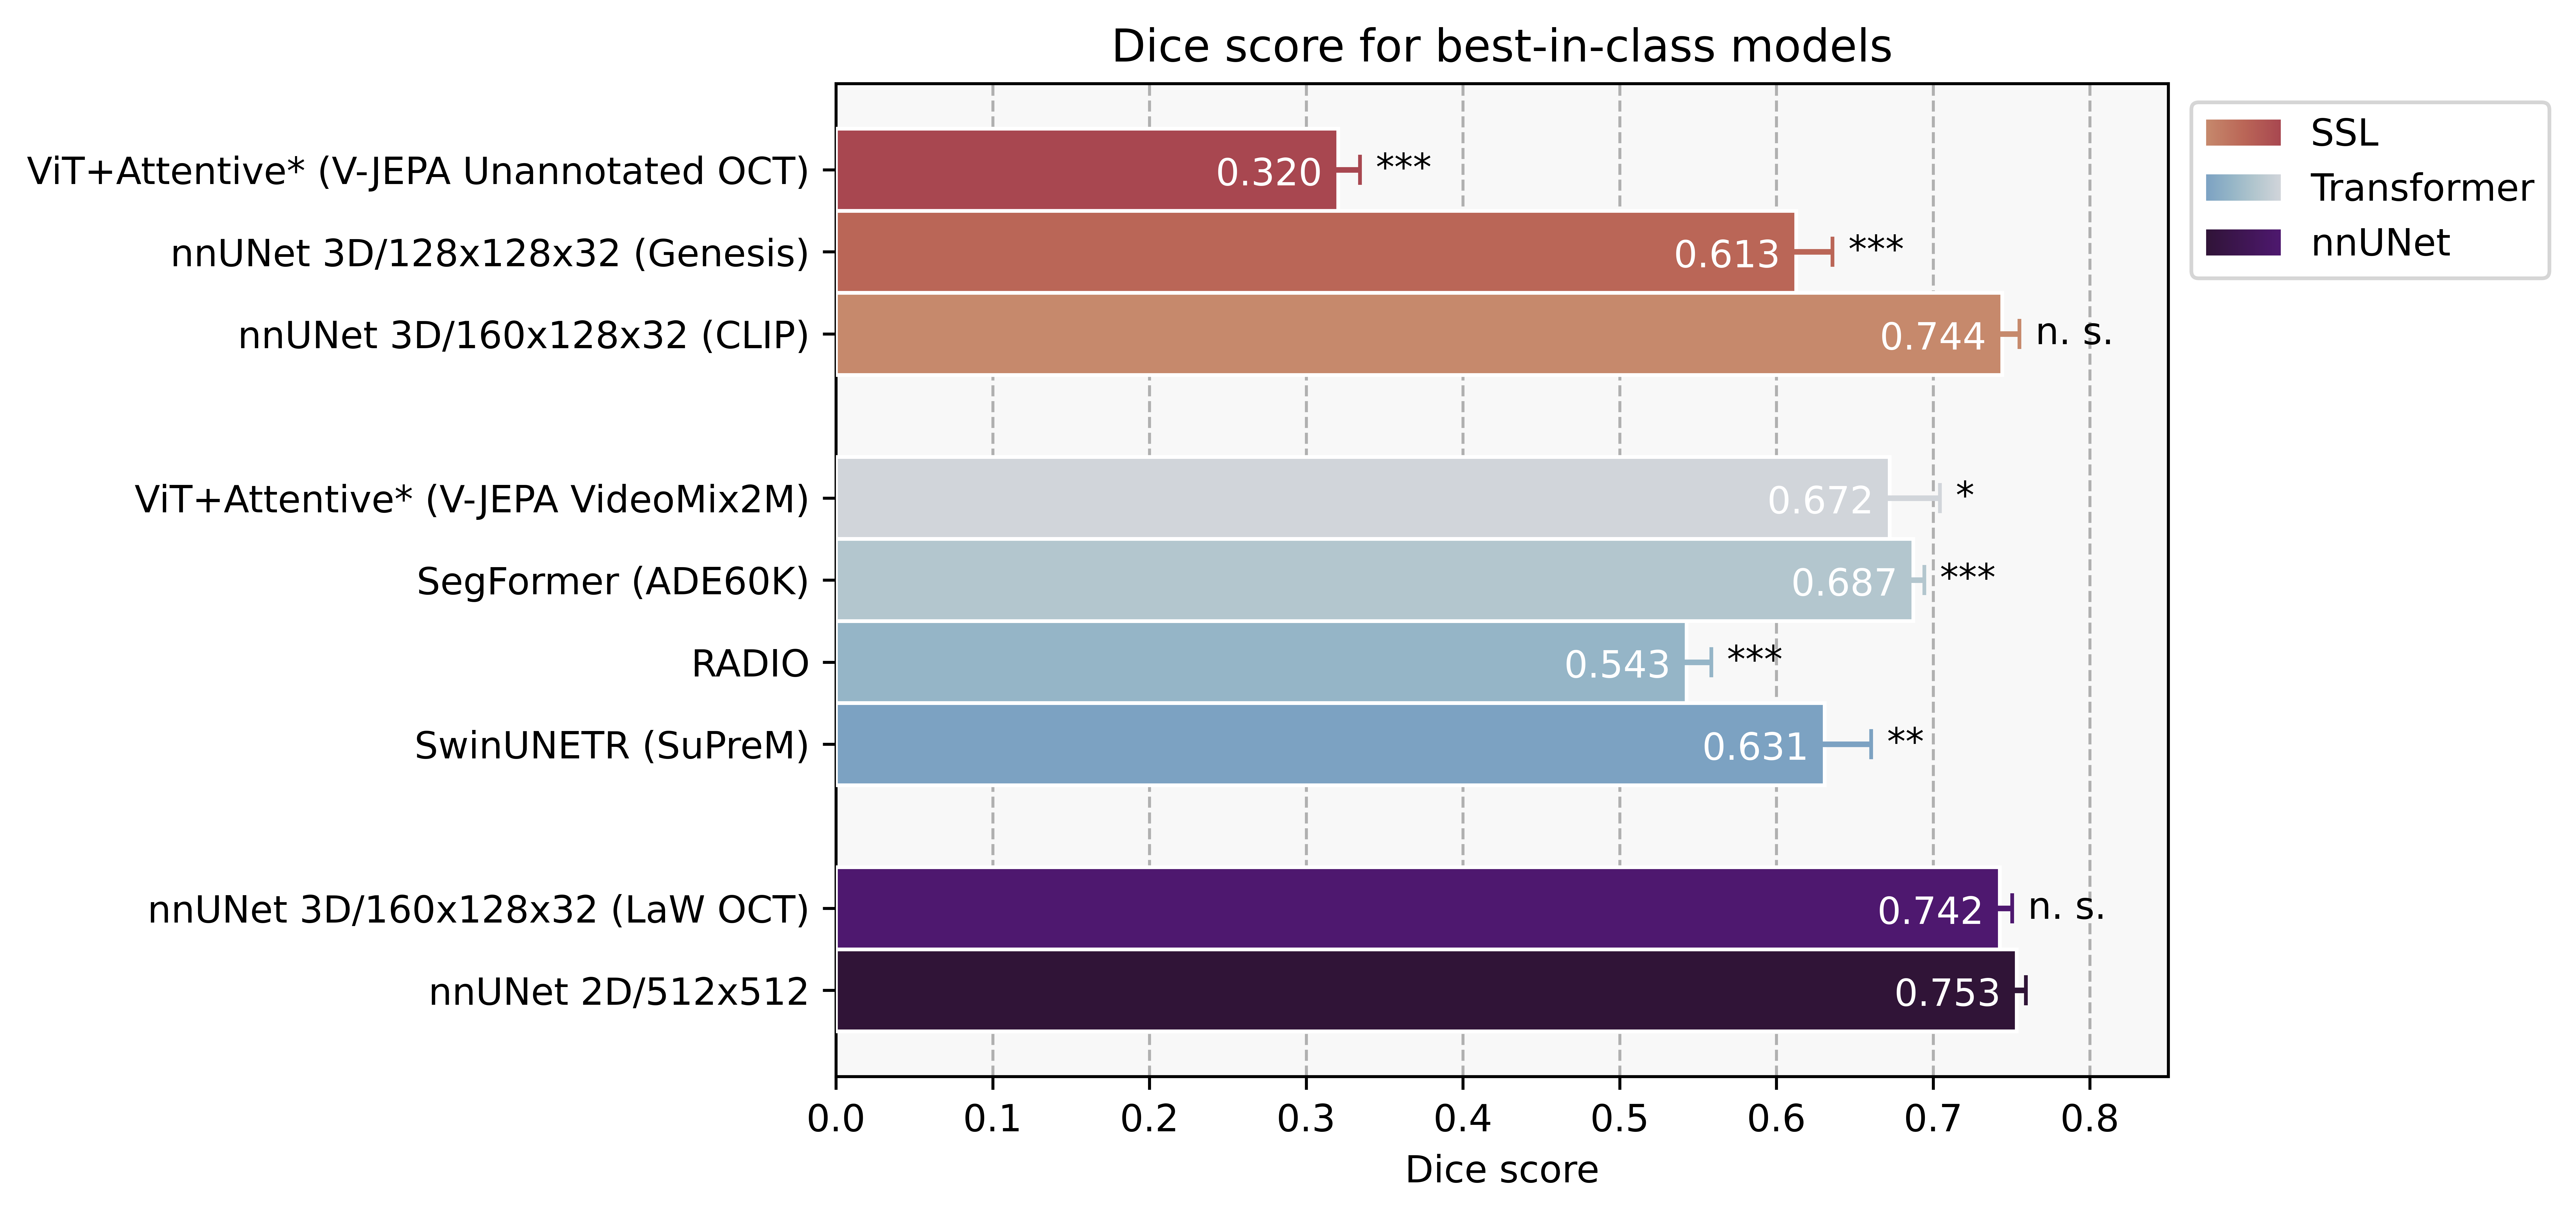
\includegraphics[width=1\textwidth]{figures/result_best_in_class_results.png}
    \caption{Summary of the results. The best model in each category is illustrated. SSL denotes self-supervised learning models, Transformer denotes transformer-based models, and nnUNet denotes 2D and 3D CNN-based nnUNet models.}
    \label{fig:results}
\end{figure}

In the SSL category, V-JEPA pre-trained on unannotated OCT images performs significantly worse than 2D nnUNet. As discussed in the previous section, the scale of the dataset may play an important role in transformer-based self-supervised learning. Genesis pre-training on unannotated OCT images also performs significantly worse than the 2D nnUNet. However, it performs comparably to the best 3D nnUNet pre-trained on the LaW OCT dataset. Although it is not comparable to the best-performing model, it is as effective as supervised pre-training while not requiring additional annotations. CLIP pre-training on co-registered multi-modal OCT images performs comparably to the 2D nnUNet model. Additionally, it performs comparably to the 3D nnUNet model pre-trained on the LaW OCT dataset. This demonstrates that CLIP can be as effective as supervised pre-training while being less costly in terms of annotation.

Our experiments show that the Dice scores of transformer-based models are significantly lower than those of the 2D nnUNet. Transformers utilize a self-attention mechanism that enables the model to combine features from different parts of the image. In contrast, the kernels of CNNs are designed to learn local features. Since calcium plaques are typically located around artery walls, CNNs are more suitable for detecting them. Additionally, the scale of the dataset used in self-supervised learning may play an important role. The nnUNet, on the other hand, is designed for small to medium-sized medical datasets. Scaling up the size of the dataset and model parameters may not be advantageous for CNNs after a certain point. In contrast, transformers are likely to benefit from scaling~\cite{Zhai2021}. This study does not aim to prove that nnUNet is better than transformers in general. It only demonstrates that nnUNet is more suitable for calcium segmentation on OCT images with the current scale of the dataset and model parameters.

The best model in our study is 2D nnUNet, which achieved an average Dice score of $0.753\pm0.006$. However, continuity is better achieved and retained during the post-processing with 3D segmentation than the 2D counterpart. 2D nnUNet, on the other hand, does not benefit from pre-training on other datasets, because converting the dataset into 2D images provides sufficient samples for the model to learn the features of the calcium plaques. In contrast, the best performance in the 3D nnUNet is achieved by pre-training on the LaW OCT dataset. The patch size of 3D nnUNet is crucial for the model's performance. Reducing the patch size in the depth dimension significantly enhances the performance, whereas increasing context in the width and height dimension does not. This reflects the nature of annotating calcium plaques in OCT images. Calcium plaques are identified by changes in intensity around the artery walls. Therefore, the x-y plane context does not provide additional information to the model. Similarly, calcium often occurs between adjacent slices, so there is no need for the model to have more context in the depth dimension.

\section{Discussion}
\subsection{Scale Analysis}
We conducted a study on the scale of the dataset used to train the model and its effect on model performance. We randomly subsampled 33\%, 50\%, 66\%, and 83\% of the Calcium OCT dataset while excluding the test set. Each sampled dataset was split into 75\% and 25\% for training and validation respectively. We then trained the model with the training set, while tracking the best model with the validation set. The final Dice score and cross entropy loss are calculated using the test set which remains the same across all scales and experiments.

It is worth pointing out that, in the Calcium OCT dataset, the outcome of the model is highly sensitive to the selection of training data. This is unsurprising as the total size of the dataset is particularly small. This reflects on the standard deviation and the scores volatility, as the scale increases.

\begin{figure}[hbt]
    \centering
    \begin{subfigure}[t]{0.49\textwidth}
        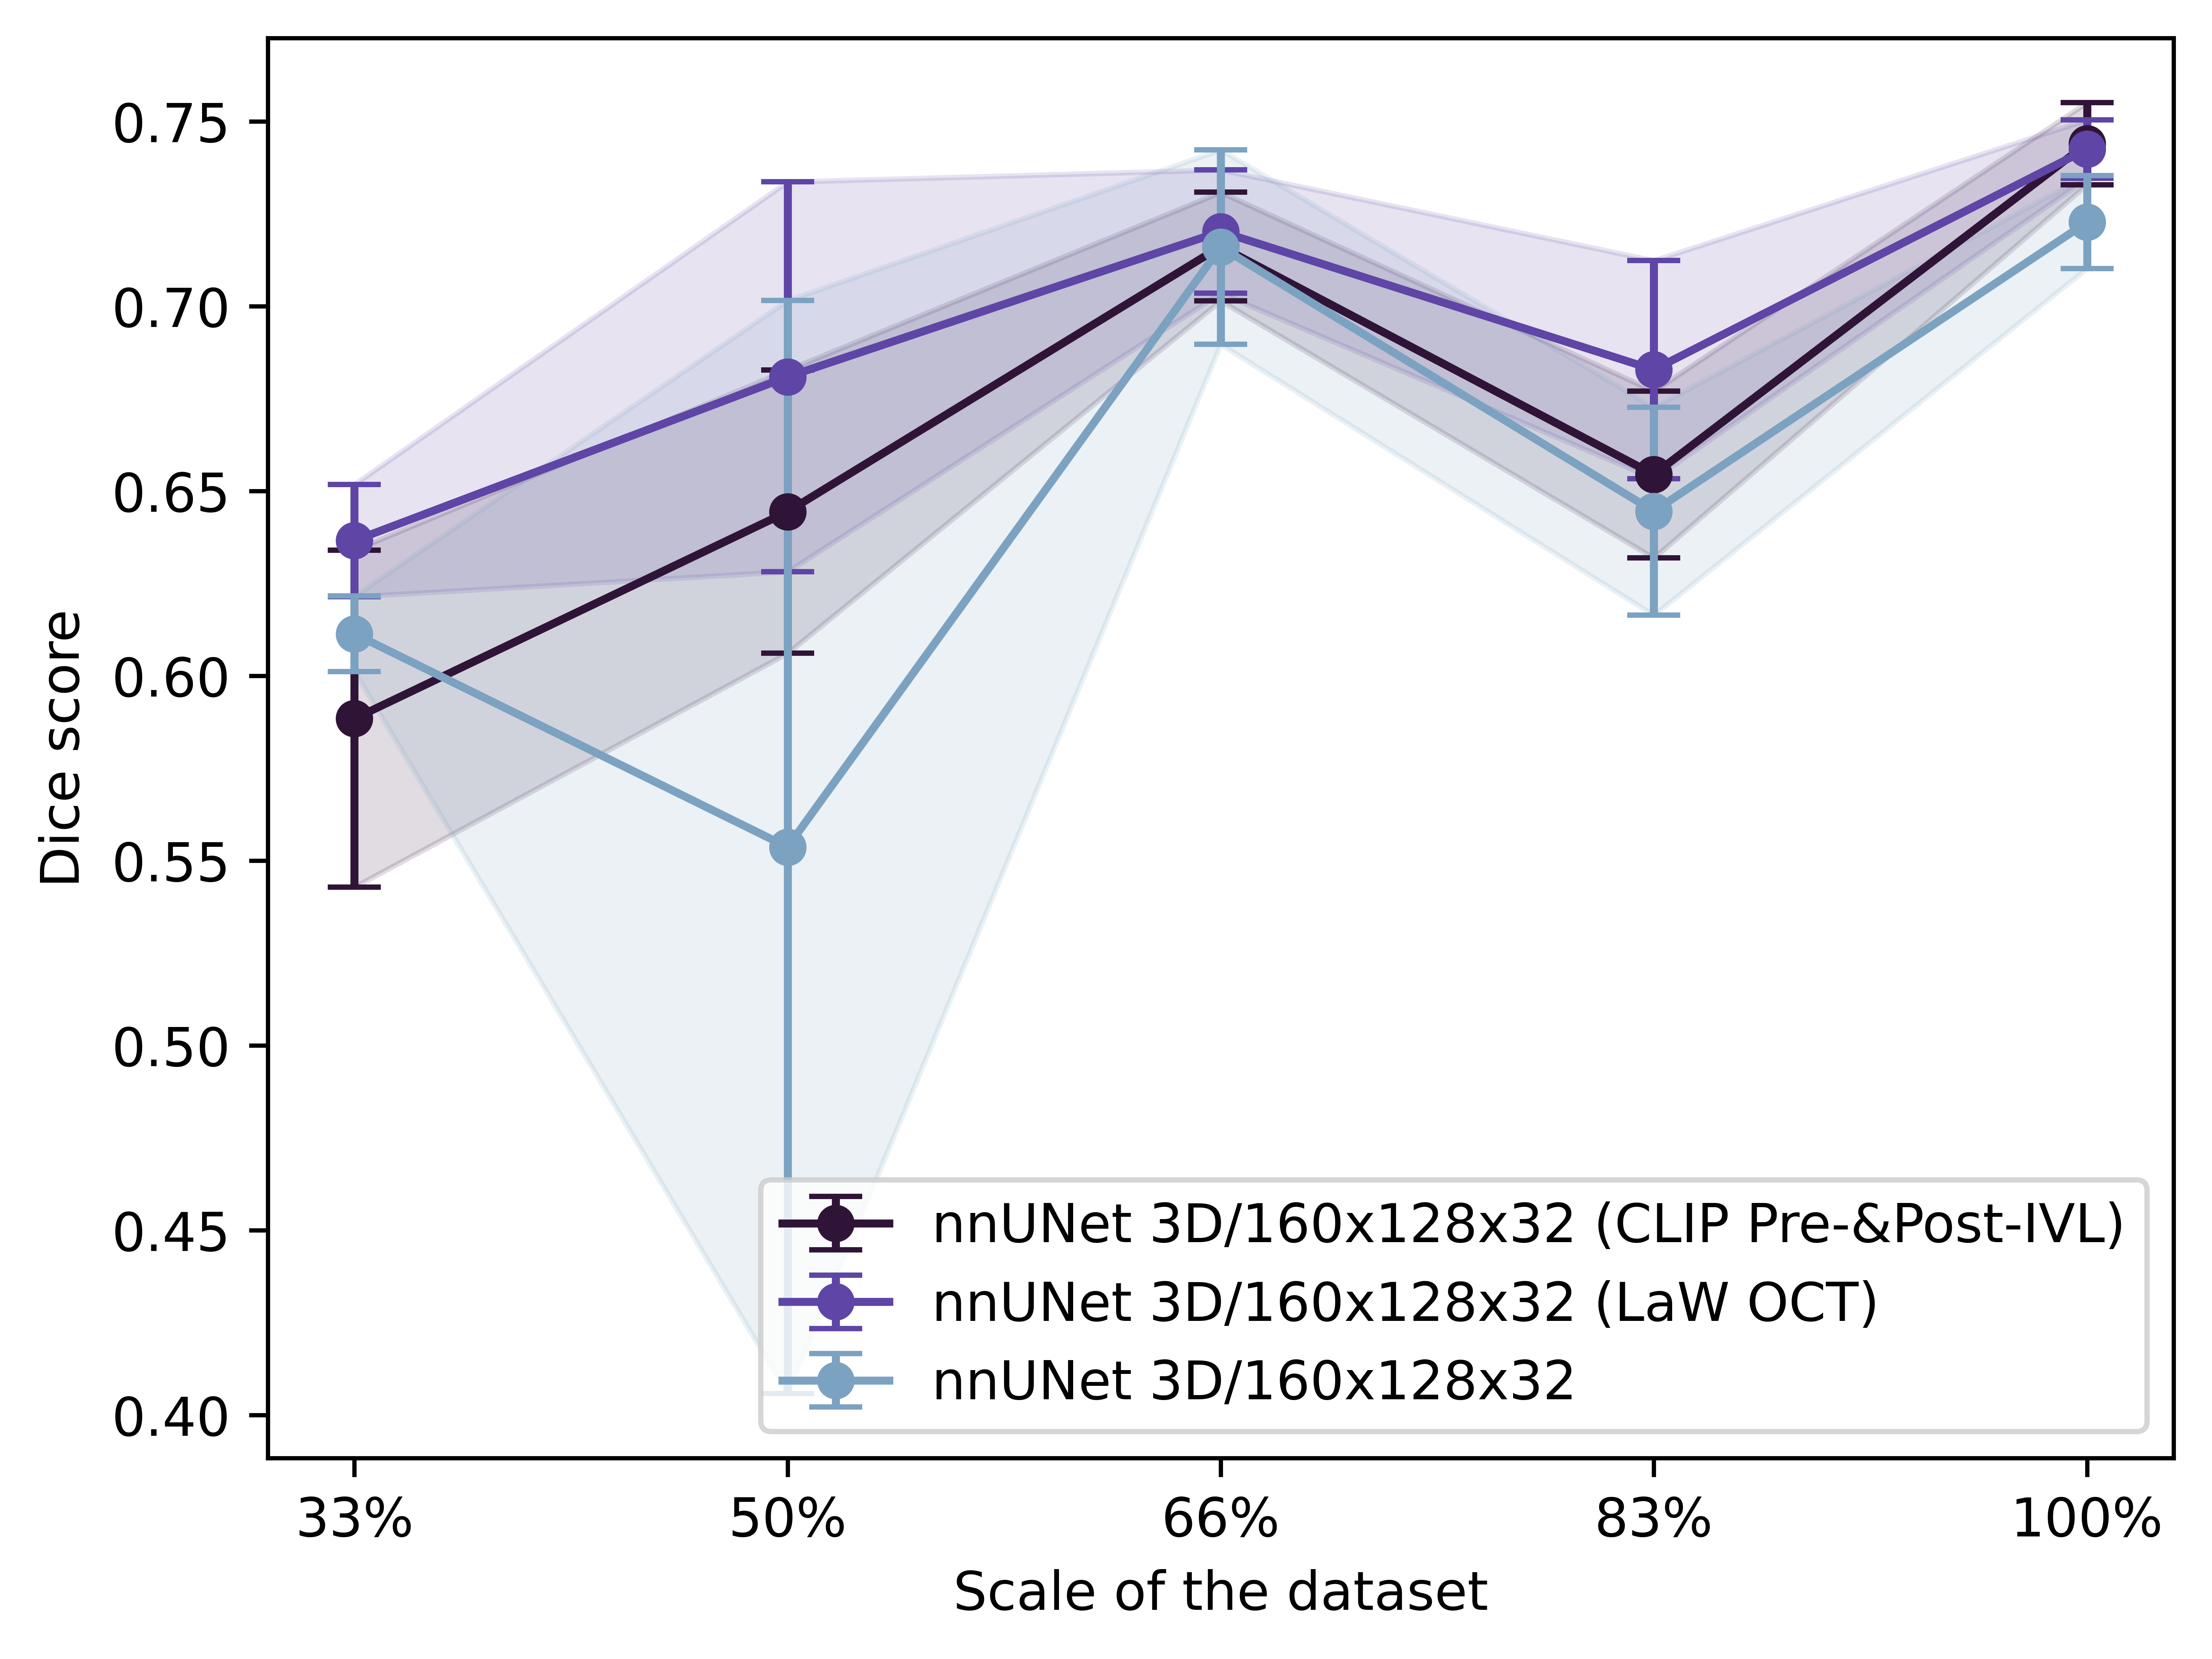
\includegraphics[width=1\linewidth]{figures/discussion_scale_analysis.png}
        \caption{Dice score scale analysis.}
        \label{fig:scale-analysis}
    \end{subfigure}%
    \begin{subfigure}[t]{0.49\textwidth}
        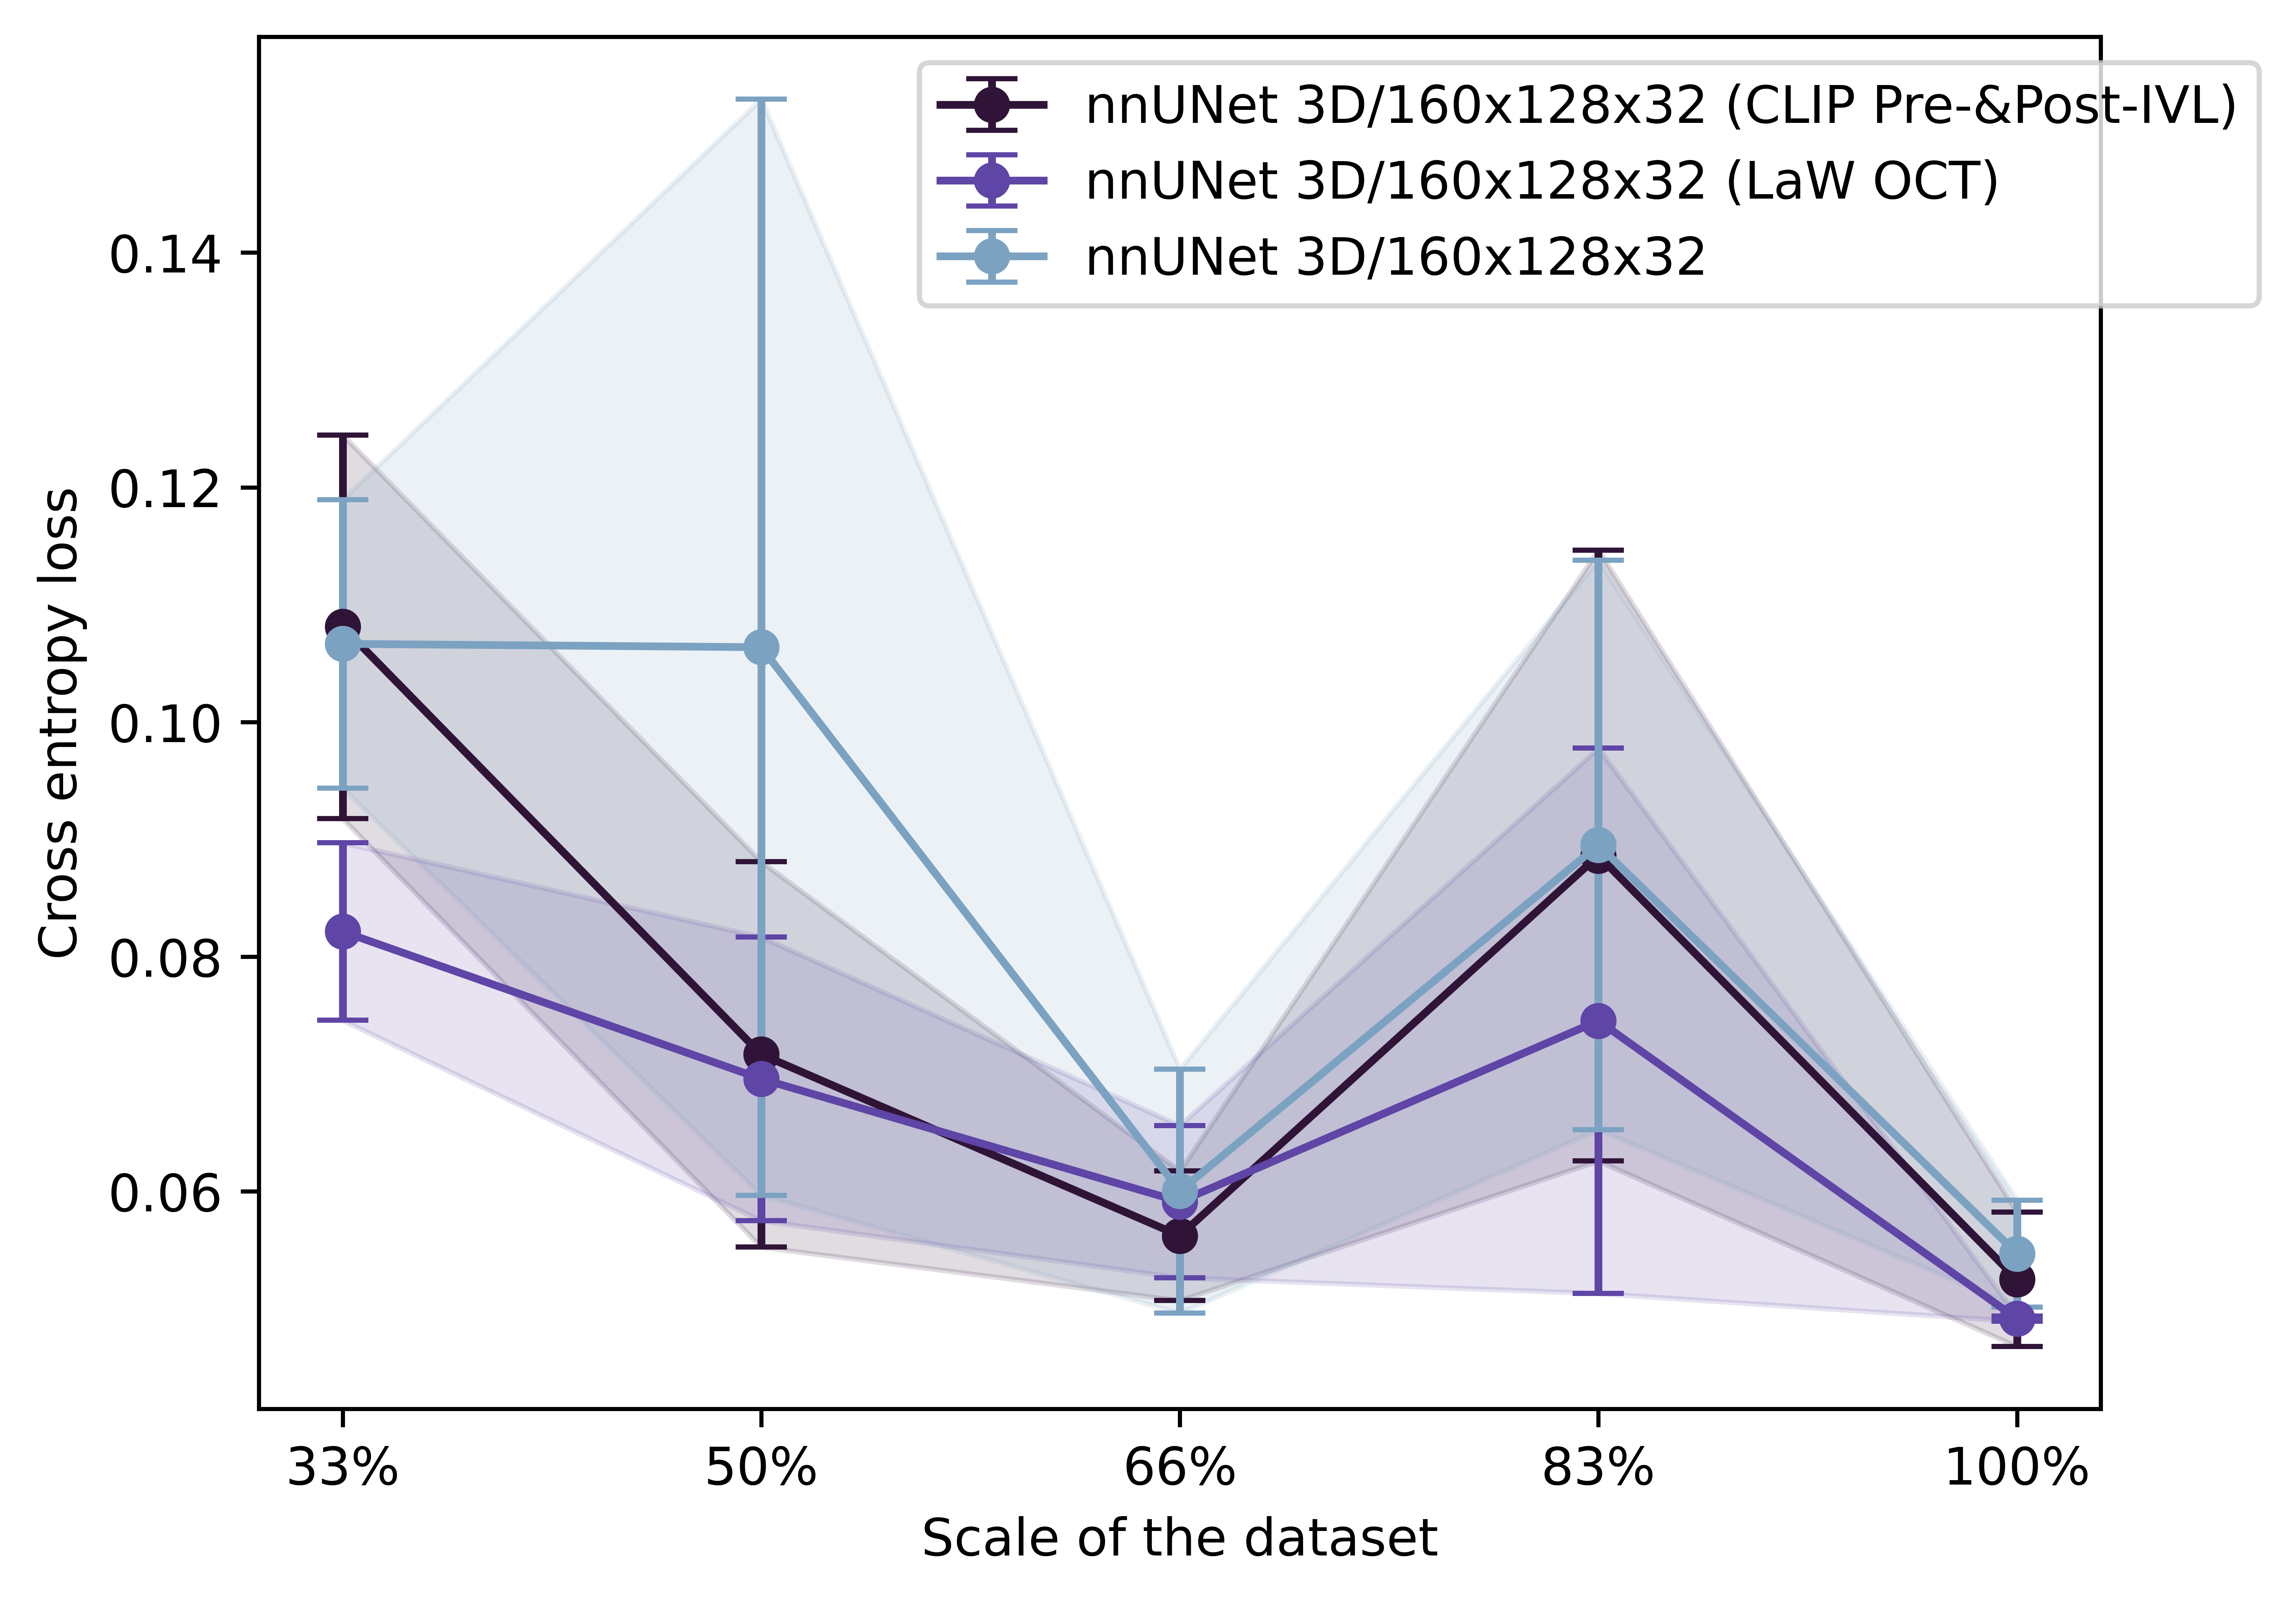
\includegraphics[width=1\linewidth]{figures/discussion_cross_entropy_scale_analysis.png}
        \caption{Cross entropy loss scale analysis.}
        \label{fig:cross-entropy-scale-analysis}
    \end{subfigure}
    \caption{Scale analysis of 3D nnUNets trained on the Calcium OCT dataset, subsampled at different scales. The values are shown in a moving average with a window size of 3.}
\end{figure}

As shown in Figure~\ref{fig:scale-analysis}, supervised pre-training on the LaW OCT dataset is more reliable than self-supervised learning on a smaller dataset, resulting in a lower standard deviation and a higher averaged Dice score. Conversely, CLIP is less effective than supervised pre-training, yet it is more beneficial than not having any pre-training.

The model's confidence and its correctness can be quantified using cross entropy loss. When the model is highly confident of its prediction and the prediction is correct, the loss is low. In contrast, when the model is confident of its incorrect prediction, the loss is high. The mathematical definition of cross entropy loss is defined below

\begin{equation}
-\frac{1}{N}\sum_{i=1}^{N}\left[y_{i}\cdot\log\left(p(y_{i})\right)+ \left( 1-y_{i} \right)\cdot \log\left(1 - p(y_{i})\right) \right]
\end{equation}

As shown in Figure~\ref{fig:cross-entropy-scale-analysis}, supervised pre-training on the LaW OCT dataset and CLIP can bolster the correctness and confidence of the 3D nnUNet. Although CLIP may be less effective than its pre-training counterpart, it costs less and can serve as an alternative option to improve prediction confidence and accuracy in a resource-limited environment.
% We hypothesize two possible scenarios. One scenario is that eight volumes, with four training, two validation, and two testing volumes, are already in a low data regime.  Further studying them does not reflect what other self-supervised learning research has shown, which is that SSL is effective in low-data regimes. The other 
One possible scenario is that CLIP features are not as effective as supervised pre-training features. CLIP implicitly learns the features of the lumen and wall, while supervised pre-training explicitly learns those features. This leads to more data being needed for CLIP to translate the implicit features into the explicit features, as we see CLIP thrive as the scale of the dataset increases. 
% We recommend conducting more studies on the scale of the dataset, as this study is only preliminary and may not be conclusive.

\subsection{Visually Good Features}
Visually good features do not always lead to better performance, as the distinction of the most important features weighs more than their aesthetics. We visualize the features from V-JEPA (VideoMix2M) and the features from the ViT initial weights. Shown in Figure~\ref{fig:visually-good-features}, both retain the structure of the artery walls. However, the features from V-JEPA (VideoMix2M) put the background into the same cluster and give more distinction to the artery walls. This may explain why V-JEPA (VideoMix2M) improves the model's performance. While the features from the initial weights of the model retain the original structure and the artery walls are visible to the human eye, a closer look at the color of the features shows that the artery walls are not as distinguishable from the background or other structures, as they blend into a gradient of colors. Features that appear good to human eyes may not be the best for the model to learn from.

\begin{figure}[hbt]
    \centering
    \begin{subfigure}[t]{0.8\textwidth}
        \centering
        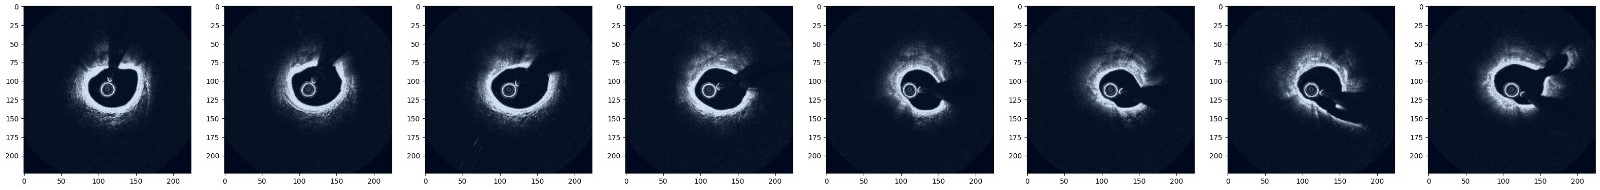
\includegraphics[width=0.9\linewidth]{figures/discussion_visual_vjepa_input.jpg}
        \caption{Input image}
    \end{subfigure}\\
    \begin{subfigure}[t]{0.8\textwidth}
        \centering
        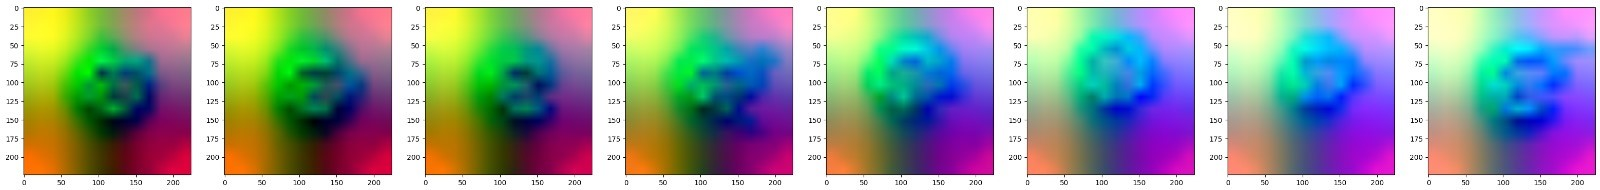
\includegraphics[width=0.9\linewidth]{figures/discussion_visual_vjepa_initial.jpg}
        \caption{PCA feature from ViT with initial weight}
    \end{subfigure}\\
    \begin{subfigure}[t]{0.8\textwidth}
        \centering
        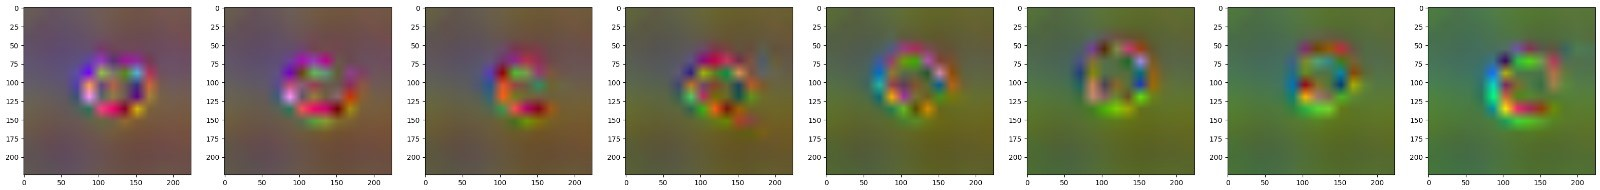
\includegraphics[width=0.9\linewidth]{figures/discussion_visual_vjepa_pretrained.jpg}
        \caption{PCA feature from ViT with V-JEPA pre-trained weight}
    \end{subfigure}
    \caption{PCA of the output features from the initial weight of the model and the features learned by V-JEPA. The volume is unrolled along the depth dimension.}
    \label{fig:visually-good-features}
\end{figure}

Visualizing ViT (RADIO) features also supports this hypothesis. Shown in Figure~\ref{fig:radio-features}, features from ViT (RADIO) are humanly interpretable, as they can successfully distinguish OCT image semantics. The border between the background and the regions where the waves could travel is visible. However, the features of the artery walls are not as distinct. This may explain why ViT (RADIO) does not perform well in terms of Dice score.

\begin{figure}[hbt]
    \centering
    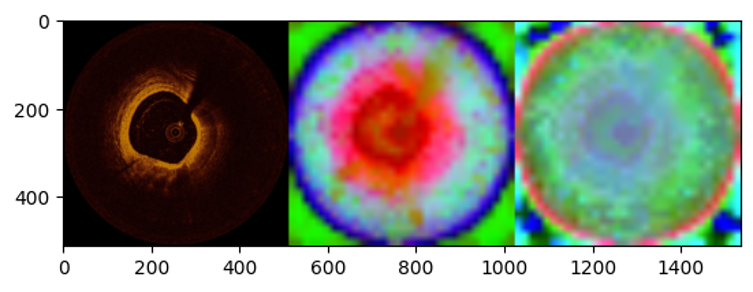
\includegraphics[width=0.35\textwidth]{figures/discussion_radio_feature.png}
    \caption{PCA of the output features from ViT (RADIO). The middle column shows the PCA of the features with the first principal component kept. The right column shows the PCA with the first principal component removed.}
    \label{fig:radio-features}
\end{figure}

\subsection{V-JEPA Pre-training}
Unlike Genesis, where loss and semantic checks of the model's learning on the pre-text task can be easily determined, V-JEPA does not provide such clarity. We experimented with different configurations of V-JEPA pre-training on our unannotated OCT images. We faced difficulties in converging the loss. As shown in Figure~\ref{fig:v-jepa-training}, the loss curve of ViT-L (V-JEPA Unannotated OCT) is converging, but it is sensitive to the configurations used.

\begin{figure}[hbt]
    \centering
    \begin{subfigure}[t]{0.3\textwidth}
        \centering
        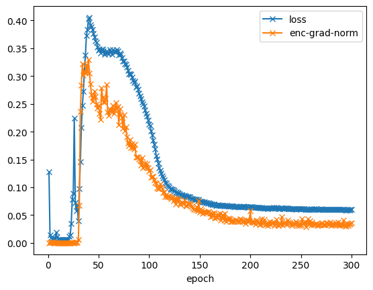
\includegraphics[width=0.9\linewidth]{figures/discussion_vjepa_training_1.png}
        \caption{ViT-L (V-JEPA Unannotated OCT)}
    \end{subfigure}%
    \begin{subfigure}[t]{0.3\textwidth}
        \centering
        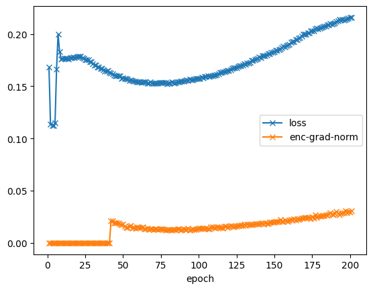
\includegraphics[width=0.9\linewidth]{figures/discussion_vjepa_training_2.png}
        \caption{ViT-S (V-JEPA Unannotated OCT)}
    \end{subfigure}%
    \begin{subfigure}[t]{0.3\textwidth}
        \centering
        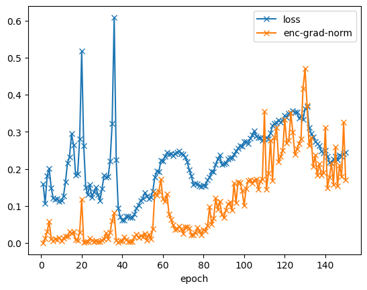
\includegraphics[width=0.9\linewidth]{figures/discussion_vjepa_training_3.png}
        \caption{ViT-L (V-JEPA Unannotated OCT) with more weight decay}
    \end{subfigure}
    \caption{Loss curves of V-JEPA pre-training on unannotated OCT images with various configurations.}
    \label{fig:v-jepa-training}
\end{figure}

One way to determine V-JEPA convergence is to plot the hidden features from the target encoder and compare them to those from the context encoder. As illustrated in Figure~\ref{fig:v-jepa-prediction}, the pre-training can succeed in the V-JEPA pre-text task of predicting the hidden features of the masked-out parts of the video. In contrast to Genesis or other pixel-level prediction pre-text tasks, it cannot be easily determined if the prediction is correct since it is only an embedding vector. This is the trade-off of using V-JEPA: it is more computationally efficient than pixel-level pre-text tasks but makes it harder to determine if the model is learning correctly.

\begin{figure}[hbt]
    \centering
    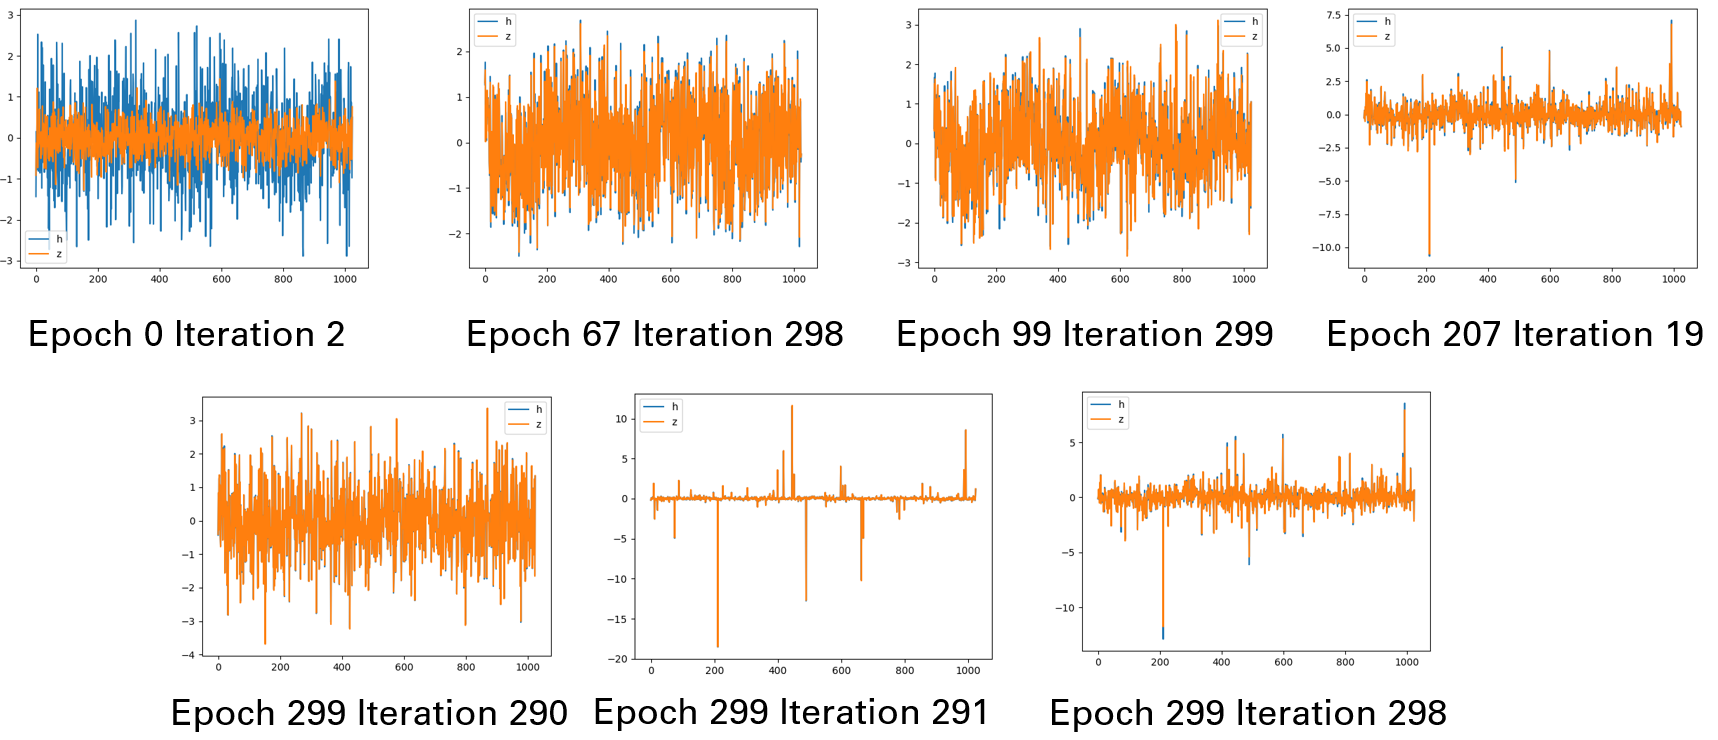
\includegraphics[width=0.8\textwidth]{figures/discussion_vjepa_prediction.png}
    \caption{Hidden features from target encoder (blue) and context encoder of ViT (V-JEPA Unannotated OCT) (orange) over training epochs. The bottom row shows different hidden features from the target encoder and context encoder in the final epoch.}
    \label{fig:v-jepa-prediction}
\end{figure}

\subsection{CLIP Pre-training}\label{sec:results:discussion:clip}
As mentioned in Section~\ref{sec:implementation:clip}, CLIP requires a shared encoder and projector for the pre-training to converge. In this section, we present the sanity checks performed and the results, providing insights for future works that may aim to adapt CLIP to multi-modalities of OCT images.

We first performed a sanity check of CLIP by training the model to match the same images, as shown in Figure~\ref{fig:clip-sanity-check-same-image}. This is a much simpler problem, and configurations that cannot match the same image will not be able to match co-registered multi-modal OCT images. Next, we trained the model to match the Pre-IVL and Post-IVL images, as shown in Figure~\ref{fig:clip-sanity-check-different-image}. This is the main task of CLIP. We found that only a shared encoder and projector can effectively converge the losses.

\begin{figure}[hbt]
    \centering
    \begin{subfigure}[t]{0.3\textwidth}
        \centering
        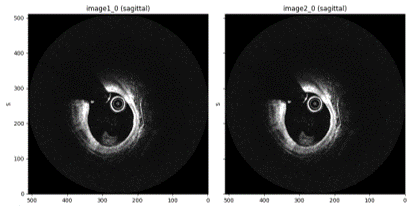
\includegraphics[width=0.9\linewidth]{figures/discussion_clip_same_image.png}
        \caption{Same images}
        \label{fig:clip-sanity-check-same-image}
    \end{subfigure}%
    \begin{subfigure}[t]{0.3\textwidth}
        \centering
        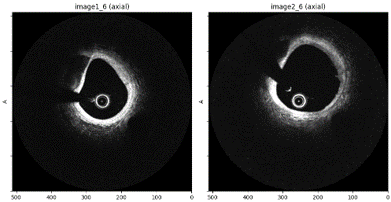
\includegraphics[width=0.9\linewidth]{figures/discussion_clip_pre-ivl_post-ivl_image.png}
        \caption{Pre-IVL and Post-IVL}
        \label{fig:clip-sanity-check-different-image}
    \end{subfigure}\\
    \begin{subfigure}[t]{0.3\textwidth}
        \centering
        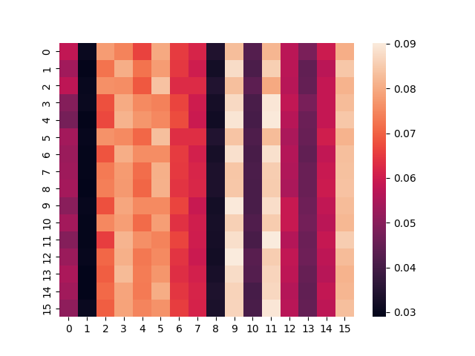
\includegraphics[width=0.9\linewidth]{figures/discussion_clip_same_image_diff_enc_diff_proj_logits.png}
        \caption{Co-similarity matrix of different encoders and projectors on the same images.}
        \label{fig:clip-cosimilarity-diff-enc-proj}
    \end{subfigure}%
    \hfill
    \begin{subfigure}[t]{0.3\textwidth}
        \centering
        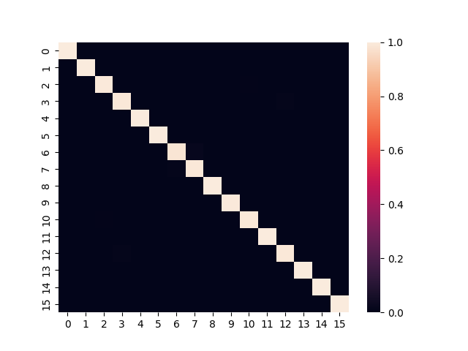
\includegraphics[width=0.9\linewidth]{figures/discussion_clip_same_image_diff_enc_shared_proj_logits.png}
        \caption{Co-similarity matrix of different encoders and shared projectors on the same images.}
        \label{fig:clip-cosimilarity-same-enc-proj}
    \end{subfigure}%
    \hfill
    \begin{subfigure}[t]{0.3\textwidth}
        \centering
        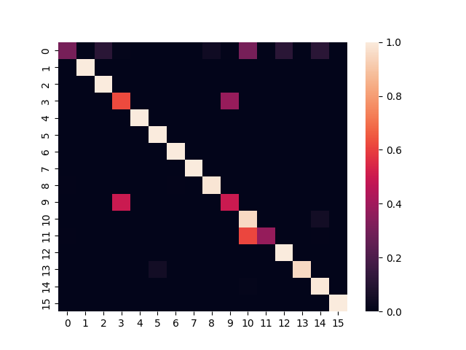
\includegraphics[width=0.9\linewidth]{figures/discussion_clip_same_image_shared_enc_shared_proj_logits.png}
        \caption{Co-similarity matrix of shared encoders and projectors on different modalities.}
        \label{fig:clip-cosimilarity-shared-enc-proj}
    \end{subfigure}
    \caption{Sanity check of CLIP. The model is trained to match the same images.}
    \label{fig:clip-sanity-check}
\end{figure}

To determine whether the model is learning, we can plot a co-similarity matrix of the features output by the model. As shown in Figure~\ref{fig:clip-cosimilarity-diff-enc-proj}, when using different encoders and projectors, the loss did not converge, and the matrix did not resemble an identity matrix. In contrast, with a shared projector, the loss converged using the same images. The co-similarity matrix resembled an identity matrix, as shown in Figure~\ref{fig:clip-cosimilarity-same-enc-proj}. However, it did not converge when training on different image modalities. Only shared encoders and projectors could converge when training on different image modalities. Their co-similarity matrix appeared close to an identity matrix, as shown in Figure~\ref{fig:clip-cosimilarity-shared-enc-proj}.

Unlike language and image, different OCT image modalities are not as distinct. Thus, learning to align hidden features with different encoders and projectors may introduce noises during the initial training phase, preventing the model from converging. 
%%%%%%%%%%%%%%%%%%%%%%
\chapter{Related Work}
%%%%%%%%%%%%%%%%%%%%%%

% The related work section covers closely related work. Here you can highlight
% the related work, how it solved the problem, and why it solved a different
% problem. Do not play down the importance of related work, all of these
% systems have been published and evaluated! Say what is different and how
% you overcome some of the weaknesses of related work by discussing the 
% trade-offs. Stay positive!

% This section is usually 3-5 pages.

% Self-supervised learning
\section{Self-supervised learning}
Self-supervised learning (SSL) has been proven to be a promising approach for natural language processing tasks (NLP). SSL can be split into two parts which are pre-text tasks and downstream tasks. Pre-text tasks are tasks that are designed to learn representations from the data itself without human annotations. Downstream tasks are finetuning tasks that use the learned representations from pre-text tasks to solve the tasks that require human annotations. It allows models to learn representations while avoiding the costs of human annotations~\cite{Jaiswal2020}. Unsupervised pre-text tasks are not uncommon in the computer vision (CV) domain. For example, autoencoder~\cite{Hinton2006}, denoising autoencoder~\cite{Vincent2008}, and colorization~\cite{Larsson2017} are some of the pre-text tasks that have been used in CV. However, suitable pre-text tasks for SSL in computer vision are still under research.

% Self-supervised learning in CVs
In recent years, discriminative and generative tasks have been proposed as pre-text tasks for the CV field. SimCLR~\cite{Chen2020Simple} is a discriminative method that learns representations by maximizing the similarity between differently augmented views of the same image and minimizing the similarity between views of different images. This is also known as contrastive learning (CL). Representations learned from SimCLR have shown to be effective for classification tasks, outperforming supervised learning on ImageNet~\cite{Russakovsky2015} using the same architecture ResNet50~\cite{He2016}. SimCLRv2~\cite{Chen2020} is an improvement of SimCLR using a larger encoder, projection head, and momentum contrast (MoCo)~\cite{He2020} that uses a queue and a moving average encoder to stabilize the training. Nevertheless, contrastive learning methods require a large batch size and a large number of negative samples to work effectively~\cite{Chen2020Simple}. This makes it difficult to scale to large datasets and models. 

In contrast to contrastive learning, masked autoencoding (MAE) learns representations by generating pixel values of the masked-out parts of images, honing a similar spirit to masked language modeling (MLM)~\cite{Devlin2019} in NLP. It has been preliminarily explored on the vision transformer (ViT) model at the same time the architecture has been proposed~\cite{Dosovitskiy2020vit}. However, the performance of masked autoencoding in the original paper is not as good as supervised learning. To make this work, He et al.~\cite{He2022} propose masking out 75\% of an image rather than 50\% experimented previously. Furthermore, an asymmetric encoder-decoder architecture of MAE is introduced. An encoder operates only on the visible pixels and a lightweight decoder operates on the encoded tokens as well as the mask tokens presented afterwards. Compared to CL, batch size, data augmentation and number of negative samples are not as critical for MAE, rendering it more scalable. MAE outperforms supervised learning and supervised pre-training on ImageNet using the same architecture ViT. Additionally, MAE has been evaluated on semantic segmentation on ADE20k~\cite{Zhou2018}, highlighting that it can be used for dense prediction downstream tasks as well. Nonetheless, working at a pixel level, MAE is computationally expensive compared to CL.

Like MAE, the bidirectional encoder for image transformer (BEiT) first learns the image patch tokenizer and predicts the tokenized values of the mask tokens instead of the pixel values as in MAE~\cite{Bao2022beit}. BEiT has been shown to outperform supervised learning and supervised pre-training on ImageNet~\cite{Russakovsky2015}. It has also been evaluated on semantic segmentation on ADE20k achieving state-of-the-art performance at that time. As BEiT requires a tokenizer to be learned, it adds more complexity to the pre-text task compared to MAE. Combining restorative and discriminative pre-text tasks, DINOv2~\cite{Oquab2024dinov} proposes to learn representations by predicting the tokenized values of the mask tokens as well as matching the class tokens of teacher and student networks on different crops of the same image. This approach has been shown to outperform other image SSLs at the time. Performing representation learning at the token level allows DINOv2 to be more efficient than pixel-level SSLs. In addition, I-JEPA~\cite{Assran2023} adapts this idea one step further. Attempting to find the most efficient approach to learning feature representations, I-JEPA proposes to predict directly the encoded vectors of mask tokens instead of the tokenized values. Evaluated on image classification, I-JEPA has shown to be comparable to other SSLs while being simpler and more efficient. 

While reading texts provides a natural way to learn natural languages, visual representations are not limited to static 2D images. Striving to incorporate a temporal dimension, extensions of existing visual SSLs have been made. VideoMAE introduces tube masking to MAE~\cite{He2022} along with an extremely high masking ratio of 90\% to 90\%~\cite{Tong2022VideoMAE}. Without external data, VideoMAE demonstrates its understanding of the video achieving state-of-the-art results to supervised learning on Kinetics-400~\cite{Kay2017Kinetics} and Something-Something V2~\cite{Goyal2017Something-SomethingV2}. Generating pixel values on video imposes even more computational limitations, as one cannot efficiently fit a clip of a video with a large number of frames. V-JEPA extends from I-JEPA~\cite{Assran2023}, predicting the encoded vectors of mask tokens on video~\cite{Bardes2024Vjepa}. As JEPA is more efficient than MAE, V-JEPA is a more efficient approach to learning representations on video. Additionally, V-JEPA has been shown to outperform VideoMAE. These ideas have the potential to be applied to 3D medical images, replacing the temporal axis with the depth axis.

% Self-supervised learning in medical imaging
\section{Self-supervised learning in medical imaging}
In medical imaging, self-supervised learning would be highly beneficial as human annotations for medical images are expensive and time-consuming. However, as it is a specialized domain, recent SSL methods in CV are not yet fully explored. There are challenges in applying SSL in medical imaging. First, medical images can be in 3D, which is not commonly explored in SSL for natural which is mostly in 2D. Second, medical images can be in various modalities such as X-ray, CT, MRI, and ultrasound. Specifically, in our study, we focus on optical coherence tomography (OCT) images of arteries that are 3D and do not have any public datasets for SSL. This poses a challenge for us as there is no direct research directly addressing our problem.

% Basic rotation, jigsaw, Rubik
 Following the same idea, Song et al.~\cite{Song2022} use rotation prediction, instance discrimination, and VAE~\cite{Kingma2013}. Using VAE as a pre-text task, the model is segmentation-ready for COVID-19 infection segmentation on lung CT images. This method outperforms supervised learning on similar architecture U-Net~\cite{Ronneberger2015} and U-Net++~\cite{Zhou2020}. Approaching 3D medical images differently, Rubik's cube solving is used as a 3D pre-text task where the model learns to classify the orientation and order of a shuffled volumetric cube. Even though discriminative, Rubik's cube shows improvement in 3D segmentation in medical images ~\cite{Zhuang2019}. Jigsaw learns feature representations by predicting the correct order of shuffled patches~\cite{Noroozi2016}. Deep clustering clusters feature vectors of the image in an unsupervised manner and use these clusters as pseudo-labels for classification~\cite{Caron2018}. Applying one or multiple pre-text tasks has been the main theme in several medical imaging SSL research papers ~\cite{Zhou2021, Zhang2021, Dufumier2021}. Taleb et al. ~\cite{Taleb2020} study 5 separated 3D self-supervised learning tasks, namely predicting latent vectors of adjacent patches, predicting the location of a given patch, solving jigsaw, predicting rotation angle, and contrastive learning. In their study, predicting latent vectors of adjacent patches yields the best results in downstream tasks.

% Contrastive learning
TS-SSL~\cite{Zhang2021} proposes an SSL on 2D spectral domain optical coherence tomography (SD-OCT) images of the retina to better classify retinal anomaly. It learns representation from classification labels, and discriminative and generative tasks simultaneously. Using contrastive loss, it maximizes the similarity between rotated views or shuffled patches of the same image and minimizes the similarity between views of different images. At the same time, it uses the same representation to predict the rotation angle of the rotated views and the order of the shuffled patches. Along with these tasks, TS-SSL also uses classification labels to predict the class of the image. However, this method only works better than supervised learning when 10\% of the labels are used for training. TS-SSL is not the only method that adopts modern SSL methods for medical imaging. Dufumier et al.~\cite{Dufumier2021} add another layer to contrastive learning by using meta-data available in medical images. Specifically, they use the age of the patient to indicate the degree of similarity between different images. This method improves bipolar disorder, Alzheimer and schizophrenia classification on 3D brain MRI images. Similarly, CLIP loss~\cite{Radford2021CLIP} can be used to leverage multi-modalities for representation learning ~\cite{Hager2023}. Encouraging images and their tabular meta-data, ubiquitous in medical imaging, to have similar representations. This method has been shown to improve classification tasks on brain MR images. 

Exploring the benefits of contrastive learning in segmentation, He et al.~\cite{He2022Intra} propose intra- and inter-slice contrastive learning for point-supervised OCT fluid segmentation of the retina. The nature of this retinal OCT is 3D. While training the segmentation model with U-Net~\cite{Ronneberger2015}, the authors leverage the fact that adjacent slices of the same volume are highly correlated, and inter-slice CL is proposed to maximize the similarity between encoded vectors of adjacent slices as well as their segmentation masks. Segmentation masks are also compared with their ground truth masks and cross-entropy loss. Segmented masks are subsequently used to select the locations of small patches to be used for intra-slice CL. Intra-slice CL maximizes the similarity between encoded fluid patches and the background fluid patches. Its result outperforms other point-based segmentation methods but is not as good as fully supervised learning. Besides spatial consistency as in previous work, temporal consistency can also be imposed~\cite{Ren2022}. Given that images are taken from the same patient at different time points, temporal consistency can be used to improve the segmentation of the images. This method has been shown to improve the segmentation of brain MRI images.

% Restorative tasks
Alternatively, generative tasks have been proposed as pre-text tasks for medical imaging. Patch shuffling~\cite{Chen2019} proposes a restorative task for 2D medical images of MRI, CT, and ultrasound. First patches are randomly cut from the original image and placed in random locations. The model learns to restore the images to their original versions. This method improves the downstream segmentation tasks in a data-scarce setting. In-painting~\cite{Pathak2016} removes a part of the image and the model learns to predict the missing part. Advancing further, Genesis~\cite{Zhou2021} explores image distortion algorithms for 3D restorative pre-text tasks on CT images. Thorough experiments show that Genesis outperforms specialized 3D state-of-the-art segmentation models and other pre-text tasks including de-noising~\cite{Vincent2010}, in-painting~\cite{Pathak2016}, jigsaw~\cite{Noroozi2016}, deep clustering~\cite{Caron2018}, rubik's~\cite{Zhuang2019} and patch shuffling~\cite{Chen2019}. This establishes a new baseline for 3D SSL in medical imaging showing that mixing pre-text tasks is beneficial. Pursuing a similar concept, SwinUNTER~\cite{Tang2022} proposes a training ViT-based model with a combination of in-paining, contrastive, and rotation.

Introducing deep clustering~\cite{Caron2018} idea to Genesis~\cite{Zhou2021}, TransVW adds a classification task to the restorative task of Genesis. First, visual words are mined automatically and grouped into clusters with deep latent features. These visual words (VW) are used to be classified and restored. Visual words improve segmentation and classification tasks in some datasets compared to Genesis~\cite{Haghighi2021}. DiRA~\cite{Haghighi2024} further improves TransVW by adding the adversarial model to tell apart the restored images and the original image. Additionally, constrastive learning is used as an additional pre-text task. Combining, discriminative, restorative, and adversarial training, DiRA outperforms TransVW and train-from-scratch models. Even though TransVW and DiRA have shown to be better than Genesis, their evaluations are not as thorough. TransVW only outperforms Genesis in some datasets, while DiRA only evaluates its performance against TransVW.

A gap between pre-text tasks studied in medical imaging and those introduced in recent visual SSL research is observed. While visual SSL research has been moving towards more efficient and simpler pre-text tasks such as DINOv2~\cite{Oquab2024dinov}, MAE~\cite{He2022}, and I-JEPA~\cite{Assran2023}, medical imaging SSL research has been focusing on blending multiple pre-text tasks. An attempt to fill this gap is evident in Genesis~\cite{Zhou2021} which works on 3D medical images at a pixel level and has shown to be better than other pre-text tasks. More studies are needed to explore simpler and more efficient pre-text tasks for medical imaging, closing the gap between visual SSL and medical imaging SSL. Concurrently, a robust evaluation in medical imaging research must be done as many reported results may not be reproducible~\cite{Isensee2024}.
% Alternatives
\section{Self-supervised learning alternatives}
Self-supervised learning has a great potential in medical imaging. If simple and robust pre-text tasks can be found, they can be used to learn representations from medical images without human annotations. However, such tasks are being explored and much work on the evaluation has to be done. Alternatives are introduced to efficiently train the models with existing small medical datasets.

SuPreM suggests pre-train models with supervised learning on large annotated datasets. SuPreM collates 9,262 CT volumes, and pre-trains models to segment a subset of organs and fine-tune them on mutually exclusive subsets of organs. The experiments show that it requires less data to learn meaning representations than SSL while also providing better transferability~\cite{Li2024}.

Rather than pre-training, nnUNet proposes a self-configuring framework for medical image segmentation. The framework automatically builds a UNet-like model for 2D and 3D medical images for a given dataset. It has been shown to robustly outperform state-of-the-art models, including popular Transformer-based and Mamba-base architectures, on several medical image segmentation tasks and works well on small datasets due to its robust positive data sampling and augmentation~\cite{Isensee2020}. Follow-up work on nnUNet has been done showing that many reported results may not be reproducible due to many reasons. The study highlights that nnUNet is the consistently best-performing model on the tasks it has been evaluated on without additional data~\cite{Isensee2024}.

Previous work at IMES to segment OCT images has been done with SegFormer pre-trained with ADE20k. SegFormer is a ViT-based model that enforces multiple resolutions at different depths of the transformer. Simple MLP~\cite{Rumelhart1986} decoder heads are introduced to combine the features from different depths. The model is state-of-the-art on semantic segmentation at the time~\cite{Xie2021SegFormer}.

Taking a different approach, RADIO proposes to learn representations from already learned models. RADIO is a student model that learns to predict the same feature from multiple teacher models, including DINOv2~\cite{Oquab2024dinov}, SAM~\cite{Kirillov2023SAM} and CLIP~\cite{Radford2021CLIP}. In addition, RADIO is trained to be resolution-agnostic, allowing it to understand images at different resolutions. RADIO has been shown to provide a high-resolution feature map that can be used for downstream tasks~\cite{Ranzinger2024RADIO}. While SSLs have great potential in medical imaging, their approaches should be compared to all other existing ones to ensure a comprehensive comparison.

%%%%%%%%%%%%%%%%%%%%
\chapter{Conclusion}
%%%%%%%%%%%%%%%%%%%%

In the conclusion, you repeat the main result and finalize the discussion of
your project. Mention the core results and why as well as how your system
advances the status quo.

\cleardoublepage
\phantomsection
\addcontentsline{toc}{chapter}{Bibliography}
\printbibliography

% Appendices are optional
% \appendix
% %%%%%%%%%%%%%%%%%%%%%%%%%%%%%%%%%%%%%%
% \chapter{How to make a transmogrifier}
% %%%%%%%%%%%%%%%%%%%%%%%%%%%%%%%%%%%%%%
%
% In case you ever need an (optional) appendix.
%
% You need the following items:
% \begin{itemize}
% \item A box
% \item Crayons
% \item A self-aware 5-year old
% \end{itemize}

\end{document}